% arara: makeindex

% Template for IEEE papers
%% bare_conf.tex
%% V1.4b
%% 2015/08/26
%% by Michael Shell
%% See:
%% http://www.michaelshell.org/
%% for current contact information.
%%
%% This is a skeleton file demonstrating the use of IEEEtran.cls
%% (requires IEEEtran.cls version 1.8b or later) with an IEEE
%% conference paper.
%%
%% Support sites:
%% http://www.michaelshell.org/tex/ieeetran/
%% http://www.ctan.org/pkg/ieeetran
%% and
%% http://www.ieee.org/

%%*************************************************************************
%% Legal Notice:
%% This code is offered as-is without any warranty either expressed or
%% implied; without even the implied warranty of MERCHANTABILITY or
%% FITNESS FOR A PARTICULAR PURPOSE!
%% User assumes all risk.
%% In no event shall the IEEE or any contributor to this code be liable for
%% any damages or losses, including, but not limited to, incidental,
%% consequential, or any other damages, resulting from the use or misuse
%% of any information contained here.
%%
%% All comments are the opinions of their respective authors and are not
%% necessarily endorsed by the IEEE.
%%
%% This work is distributed under the LaTeX Project Public License (LPPL)
%% ( http://www.latex-project.org/ ) version 1.3, and may be freely used,
%% distributed and modified. A copy of the LPPL, version 1.3, is included
%% in the base LaTeX documentation of all distributions of LaTeX released
%% 2003/12/01 or later.
%% Retain all contribution notices and credits.
%% ** Modified files should be clearly indicated as such, including  **
%% ** renaming them and changing author support contact information. **
%%*************************************************************************


% *** Authors should verify (and, if needed, correct) their LaTeX system  ***
% *** with the testflow diagnostic prior to trusting their LaTeX platform ***
% *** with production work. The IEEE's font choices and paper sizes can   ***
% *** trigger bugs that do not appear when using other class files.       ***                          ***
% The testflow support page is at:
% http://www.michaelshell.org/tex/testflow/

\documentclass{book}
\usepackage[quiet]{fontspec}
\usepackage[table,xcdraw,dvipsnames]{xcolor} % Used by spritegrid and others.
\usepackage[obeyspaces,spaces]{url}
\usepackage{longtable}
\usepackage{arydshln}
\usepackage{booktabs}
\usepackage{afterpage}
\usepackage{flushend}
\usepackage{titletoc}
\usepackage[toc]{appendix}
\usepackage{parskip}
\usepackage{graphicx,wrapfig}
\usepackage{float}
\usepackage{caption}
\usepackage{pdfpages}
\usepackage{tikzpagenodes}
\usepackage{imakeidx}
\usepackage[pagestyles,raggedright]{titlesec}
\usepackage[all]{nowidow}
\usepackage[bookmarks=true,linktoc=all]{hyperref}
\usepackage{tabularx}
\hypersetup{
  colorlinks   = true, %Colours links instead of ugly boxes
  urlcolor     = blue, %Colour for external hyperlinks
  % Each main .tex file configures via \titleformat the \chapter command
  % to do {\chapmtoc\insertminitoc} and \chapmtoc, as defined below, will
  % use \hypersetup{linkcolor=white} to avoid blue-on-blue TOC links
  % Besides, each main .tex file will issue the \tableofcontents command
  % between \hypersetup{linkcolor=black} and \hypersetup{linkcolor=blue}
  % This means however that if "blue" is modified here it must be modified
  % in these files too.
  linkcolor    = blue, %Colour of internal links
  citecolor   = red %Colour of citations
}
\usepackage{aeb-minitoc}
\usepackage{fix-cm}
\usepackage{textpos}
\usepackage{enumitem}
\usepackage{tcolorbox}
\tcbuselibrary{breakable,listings,skins,xparse}
%\usepackage{wrapfig}
\usepackage{needspace}
\usepackage{verbatim}
\usepackage{ean13isbn}
\usepackage{setspace}

% Use CHAPTER-PAGE page numbering to make it easier to modify chapters
% later, without messing up page number of the rest of the book.
\usepackage[auto]{chappg}

% Allow cross-references between the various books to the big The MEGA65 Book
\usepackage{xr}
\usepackage{varioref}
\usepackage{xparse}

\usepackage{colortbl}
\usepackage{adjustbox}

\externaldocument[M65Book-]{mega65-book}
% And a \ref alternative that checks if it needs to be a cross-reference to the
% MEGA65 Book instead.
\makeatletter
\newcommand{\bookref}[1]{%
    \@ifundefined{r@#1}{%
      {\em the MEGA65 Book}, \nameref{M65Book-#1} (\autoref{M65Book-#1})}{\autoref{#1}}%
}
\newcommand{\bookvref}[1]{%
    \@ifundefined{r@#1}{%
      {\em the MEGA65 Book}, \nameref{M65Book-#1} (\autoref{M65Book-#1})}{Chapter/Appendix \vref{#1}}%
}
\makeatother

% For fixed-width columns in register maps
\usepackage{array}

% Makes tables with double-ruled lines look better
\usepackage{hhline}

% Makes better use of space for reference tables in appendix
\usepackage{multicol}

% Shaded tables with alternate rows colored for better legibility
% Best used with larger tables rather than small tables
\usepackage{colortbl}
\usepackage{adjustbox}
\usepackage[strict]{changepage}

% \makecell command for forcing line breaks in table cells
\usepackage{makecell}

\newcolumntype{L}[1]{>{\raggedright\let\newline\\\arraybackslash\hspace{0pt}}m{#1}}
\newcolumntype{C}[1]{>{\centering\let\newline\\\arraybackslash\hspace{0pt}}m{#1}}
\newcolumntype{R}[1]{>{\raggedleft\let\newline\\\arraybackslash\hspace{0pt}}m{#1}}

% clear to left page for making two page tables starting on the odd page
\newcommand{\cleartoleftpage}{%
  \clearpage
  \ifodd\value{page}\hbox{}\newpage\fi
}

% Layout structures for acknowledgements pages
\input{elements/acknowledgements}

% For displaying Letter keys and the MEGA key
\input{elements/keys}

% For displaying print versions petscii character symbols
\input{elements/graphicsymbol}

% For Mega65 display of code, listings and screen activity
\input{elements/screenoutput}

% For MEGA65 screen shots with text flow
\input{elements/screenshots}

% For displaying sprite data in a grid
\input{elements/spritegrid}

% Don't number sections
\setcounter{secnumdepth}{0}

\renewcommand{\indexname}{INDEX}
\renewcommand{\appendixtocname}{APPENDICES}
\renewcommand{\appendixpagename}{APPENDICES}
\renewcommand{\appendixpage}{%
  \clearpage\thispagestyle{empty}
    \pagecolor{blue}
     \begin{center}
       {
         \large
         % Put a nice amount of vertical space before the title
         \vspace*{2cm}
               {\large\Huge\textcolor{white}{\bf{APPENDICES}}}\\
             \vspace{\fill}
       }
     \end{center}
     \newpage\pagecolor{white}\clearpage
}

\makeatletter\chardef\pdf@shellescape=\@ne\makeatother

\setcounter{tocdepth}{5}

% 1.0 cm is the distance from left of page to bullet point.
% 2.8 cm is a fudge-factor to make multi-line section names be correctly lined up.
% \@B{〈length〉} is the amount to indent prior to〈sec-num >
% \@F{〈fmt〉} is the formatting for the title heading
% \@P{〈fmt〉} is the formatting for the page number (〈pg-num〉).

\TOCLevels{chapter}{section}
\begin{minitocfmt}{\chapmtoc}
\declaretocfmt{section}{\@F{\color{white}\hypersetup{linkcolor=white}\hspace{1.0cm}\textbullet\hspace{0.25cm}\Large\bfseries}\@B{2.8cm}\@P{\mtocgobble}}
\declaretocfmt{section*}{\@F{\color{white}\hypersetup{linkcolor=white}\hspace{1.0cm}\textbullet\hspace{0.25cm}\Large\bfseries}\@B{2.8cm}\@P{\mtocgobble}}
\end{minitocfmt}

\input{fonts}

% Set margins for inner and outer pages in A5 book format
\ifdefined\printmanual
\usepackage[a5paper,nomarginpar,includemp,bottom=2cm,top=1cm,inner=1.8cm,outer=0.8cm, footskip = 1cm]{geometry}
\else
\usepackage[a5paper,nomarginpar,includemp,bottom=2cm,top=1cm,inner=1.0cm,outer=1.0cm, footskip = 1cm]{geometry}
\fi

% Some Computer Society conferences also require the compsoc mode option,
% but others use the standard conference format.
%
% If IEEEtran.cls has not been installed into the LaTeX system files,
% manually specify the path to it like:
% \documentclass[conference]{../sty/IEEEtran}

%% \input{setup}

% correct bad hyphenation here
\hyphenation{op-tical net-works semi-conduc-tor}

\makeindex[intoc]

\pagestyle{empty}

\begin{document}
\raggedbottom

% relax word wrapping with sloppy
\sloppy
% reduce overfull \hbox warnings
\hfuzz=5pt

% macro for changing the verbatim font
\makeatletter
\newcommand{\verbatimfont}[1]{\def\verbatim@font{#1}}%
\makeatother


%\pagecolor{blue}
%\clearpage\thispagestyle{empty}
%\begin{center}
%\includegraphics[width=\textwidth]{frontcover/MEGA65_logo_shadow}
%
%{\textcolor{white}{\large\Huge{\bf{USER'S GUIDE}}}}
%
%\vspace{\fill}
%\end{center}
%
\newcommand\titlestreq[3]{%
  \IfStrEq{#1}{\detokenize{#2}}{\includegraphics[height=210mm,width=149mm]{\detokenize{#3}}}{}%
}

\newcommand\titlepic[1]{%
  \titlestreq{#1}{mega65-book}{frontcover/m65book\_title}%
  \titlestreq{#1}{mega65-userguide}{frontcover/userguide\_title}%
  \titlestreq{#1}{mega65-developer-guide}{frontcover/developer\_title}%
  \titlestreq{#1}{mega65-chipset-reference}{frontcover/chipset\_title}%
  \titlestreq{#1}{mega65-basic65-reference}{frontcover/basic65\_title}%
}

\begin{tikzpicture}[remember picture,overlay,shift={(current page.north east)}]
\node[anchor=north east,xshift=0.2cm,yshift=0.1cm]{\titlepic{\jobname}};
\end{tikzpicture}

%\newpage
%\pagecolor{white}

\input{regulatory}
\input{updates}

% paper title
% Titles are generally capitalised except for words such as a, an, and, as,
% at, but, by, for, in, nor, of, on, or, the, to and up, which are usually
% not capitalised unless they are the first or last word of the title.
% Linebreaks \\ can be used within to get better formatting as desired.
% Do not put math or special symbols in the title.

\cleardoublepage

\pagenumbering{roman}

\begin{titlepage}
    \pagecolor{blue}
     \begin{center}
       {
         \large
         % Put a nice amount of vertical space before the title
         \vspace*{2cm}
               {\Huge\textcolor{white}{\bf{MEGA65 REFERENCE GUIDE}}}\\
             \vspace{\fill}
                    {\textcolor{white}
                    {Published by \\ the MEGA Museum of Electronic Games \& Art e.V., Germany.}}
       }
     \end{center}
   \end{titlepage}

% Then the copyright notice page
  \pagecolor{white}\textcolor{black}
  \vfill
  WORK IN PROGRESS

  \index{copyright}Copyright \copyright 2019 -- 2023 by Paul Gardner-Stephen,
  the MEGA Museum of Electronic Games \& Art e.V.,
  and contributors.

  This reference guide is made available under the GNU Free Documentation
  License v1.3, or later, if desired. This means that you are free to
  modify, reproduce and redistribute this reference guide, subject to
  certain conditions. The full text of the GNU Free Documentation
  License v1.3 can be found at
  \url{https://www.gnu.org/licenses/fdl-1.3.en.html}.

  Implicit in this copyright license, is the permission to duplicate
  and/or redistribute this document in whole or in part for use in
  education environments. We want to support the education of future
  generations, so if you have any worries or concerns, please contact us.

   \par\today

\newpagestyle{onlynumber}{\setfoot[][{\bf\small\thepage}][]
                                  {} {\bf\small\thepage} {}}
\pagestyle{onlynumber}
\pagecolor{white}

\hypersetup{linkcolor=black}
\tableofcontents
\hypersetup{linkcolor=blue}

%% XXX - big numbers are not in bold, because latex gets confused
\newcommand*{\justifyheading}{\raggedleft}
\definecolor{headingblue}{rgb}{0.5,0.5,1}

% \titleformat{command}[shape]
%   {format}
%   {label}
%   {sep}
%   {before}
%   [after]

% ***************
% PART title page
% ***************

\titleclass{\part}{top}
\titleformat{\part}[display]
   {\thispagestyle{empty}\pagecolor{blue}\normalfont\huge\bfseries\justifyheading}
   {\textcolor{white}{\fontsize{50}{65}\selectfont\bf{PART}\quad{\fontsize{100}{130}\selectfont \bf{\serifed\thepart}}}}
   {20pt}
   {\Huge\textcolor{white}}
   [\newpage\pagecolor{white}\textcolor{black}]

% ******************
% CHAPTER title page
% ******************

\titleformat{\chapter}[display]
   {\thispagestyle{empty}\pagecolor{blue}\normalfont\huge\bfseries\justifyheading}
   {\textcolor{white}{\MakeUppercase{\chaptertitlename}\quad{\fontsize{100}{130}\selectfont \bf\thechapter}}}
   {20pt}
   {\Huge\textcolor{white}}
   [{\chapmtoc\insertminitoc}\newpage\pagecolor{white}\textcolor{black}\cleardoublepage]

% ******************
% SECTION title page
% ******************

\titleformat{\section}[display]
   {\raggedright}
   {\thesection}
   {20pt}
   {\huge\bf\color{headingblue}\uppercase}
   [\color{black}]

\part{PREFACE}

\input{introduction}

\cleardoublepage
\pagenumbering{bychapter}

\part{GETTING TO KNOW YOUR MEGA65}

\chapter{Setup}
\phantomsection
\section{Unpacking and Connecting the MEGA65}

It is time to set up your MEGA65 home computer! The box contains the following:

\begin{itemize}
\setlength\itemsep{-0.75mm}
\item MEGA65 computer
\item Power supply (black box with socket for mains supply)
\item This book, the MEGA65 User's Guide
\item Your personal registration code, on a piece of paper (possibly tucked into the User's Guide)
\end{itemize}

In addition, to be able to use your MEGA65 computer you will need:

\begin{itemize}
\item A television or computer monitor with a VGA or digital video input, capable of displaying an image at 480p (720x480) at 60Hz or 576p (720x576) at 50Hz
\item An appropriate video cable for your display, either VGA or digital video
\end{itemize}

You may also like to use the following to get the most out of your MEGA65:

\begin{itemize}
\item A digital video display with built-in audio, or powered speakers and an appropriate audio cable with 3.5mm mini-jack connector
\item A microSD card, type SDHC, between 4GB and 32GB in size
\item An RJ45 Ethernet cable and a network router or switch
\item A fresh CR2032 battery, for the Real-Time Clock
\item A Phillips-head screwdriver, to access the inside of the case
\item A joystick or gamepad compatible with Commodore computers, with a nine-pin (DE-9) connector
\item A Commodore 1351 mouse, an Amiga mouse, or a modern replacement such as a \href{https://retrohax.net/shop/amiga/mouster/}{mouSTer} USB mouse adapter
\end{itemize}

\newpage
\section{Rear Connections}
\index{Display!Connecting}

\includegraphics[width=\linewidth]{images/illustrations/mega65-rear.pdf}
\index{Disk Drives!Connecting}
\begin{center}
\setlength{\def\arraystretch{1.5}\tabcolsep}{6pt}
\begin{longtable}{ c | l}
	1	& 	3.5mm Audio Mini-Jack \\
	2	& 	External microSD Card Slot\\
	3	& 	Network LAN Port \\
	4	& 	Digital Video Connector (including sound) \\
	5	& 	VGA Video Connector \\
	6	& 	IEC Serial Bus Connector for Disk Drives and Printers \\
	7	& 	Cartridge Expansion Port \\
	8	& 	Power Supply Socket \\
\end{longtable}
\end{center}

%\newpage
\vspace{-1cm}

\section{Side Connections}

\includegraphics[width=\linewidth]{images/illustrations/mega65-side.pdf}

\begin{center}
\setlength{\def\arraystretch{1.5}\tabcolsep}{6pt}
\begin{longtable}{ c | l}
	1	& 	Power Switch \\
	2	& 	Controller Port 2 \\
	3	& 	Controller Port 1 \\
	4	& 	Reset Button \\
\end{longtable}
\end{center}

Various peripherals can be connected to Controller Ports 1 and 2 such as
joysticks, paddles or mouse devices.

\newpage

\section{MEGA65 Screen and Peripherals}

\includegraphics[width=\linewidth]{images/illustrations/mega65-top.pdf}

To connect your MEGA65 to a display:

\begin{enumerate}
	\item Connect the power supply to the power supply socket of the MEGA65.
	\item If you have a VGA monitor and a VGA cable, connect one end to the VGA port of the MEGA65 and the other end into your VGA monitor.
	\item If you have a TV or monitor with a compatible Digital Video connector, connect one end of your cable to the Digital Video port of the MEGA65, and the other into the Digital Video port of your monitor. If you own a monitor with a DVI socket, you can use a Digital Video to DVI adapter.
\end{enumerate}

\newpage
\section{Optional Connections}
\index{Connections!IEC}
\index{SD Cards!Locations}
\begin{enumerate}
	\item The MEGA65 includes an internal 3.5" floppy disk drive. You can also connect older Commodore{\textregistered} IEC serial floppy drives to the MEGA65, such as the Commodore 1541, 1571 or 1581. To use these drives, connect one end of an IEC cable to the Commodore floppy disk drive and the other end to the Disk Drive socket of the MEGA65. You can also connect SD2IEC devices and Pi1541's. It is also possible to daisy-chain additional floppy disk drives or Commodore compatible printers.
	\item You can connect your MEGA65 to an Ethernet network using a standard Ethernet cable.
	\item For enjoying audio from your MEGA65, you can connect a 3.5mm stereo mini-jack cable to an audio amplifier or speaker system. If your system has RCA connectors you will need a 3.5mm mini-jack to twin RCA adapter cable. The MEGA65 also has a built-in amplifier to allow the use of headphones.
	\item A microSD card, type SDHC between 4GB and 32GB, can be inserted into the external microSD card slot at the rear of the MEGA65. For more information on using the microSD card slot, see ``Introducing SD Cards'' on page \pageref{sec:introducing-sd-cards}.
\end{enumerate}

\index{Real-Time Clock!Installing the Battery}
\subsection{Installing the Real-Time Clock Battery}

The MEGA65 includes a Real-Time Clock, which is used to display the time and date on the startup screen, to add timestamps to files that the MEGA65 writes to your SD cards, and by the {\bf DT\$} and {\bf TI\$} BASIC65 variables. This clock utilises a CR2032 coin-cell battery\footnote{Early models of MEGA65 with the "R3A" board revision used a battery of type CR1220 for the Real-Time Clock. Revisions "R5" and later, which began shipping in late 2023, use a CR2032 battery.} to keep time when the MEGA65 isn't switched on. The MEGA65 does not include a battery in order to avoid issues related to shipping batteries internationally.

To install the battery, use a Phillips-head screwdriver to open the case, exposing the motherboard. The case is held together with three screws, all of which are along the bottom of the front side of the case. Once the screws have been removed, carefully lift the top half of the case. Note the orientation of the keyboard connector, then disconnecting it.

The battery is located between the controller ports and the keyboard connector.

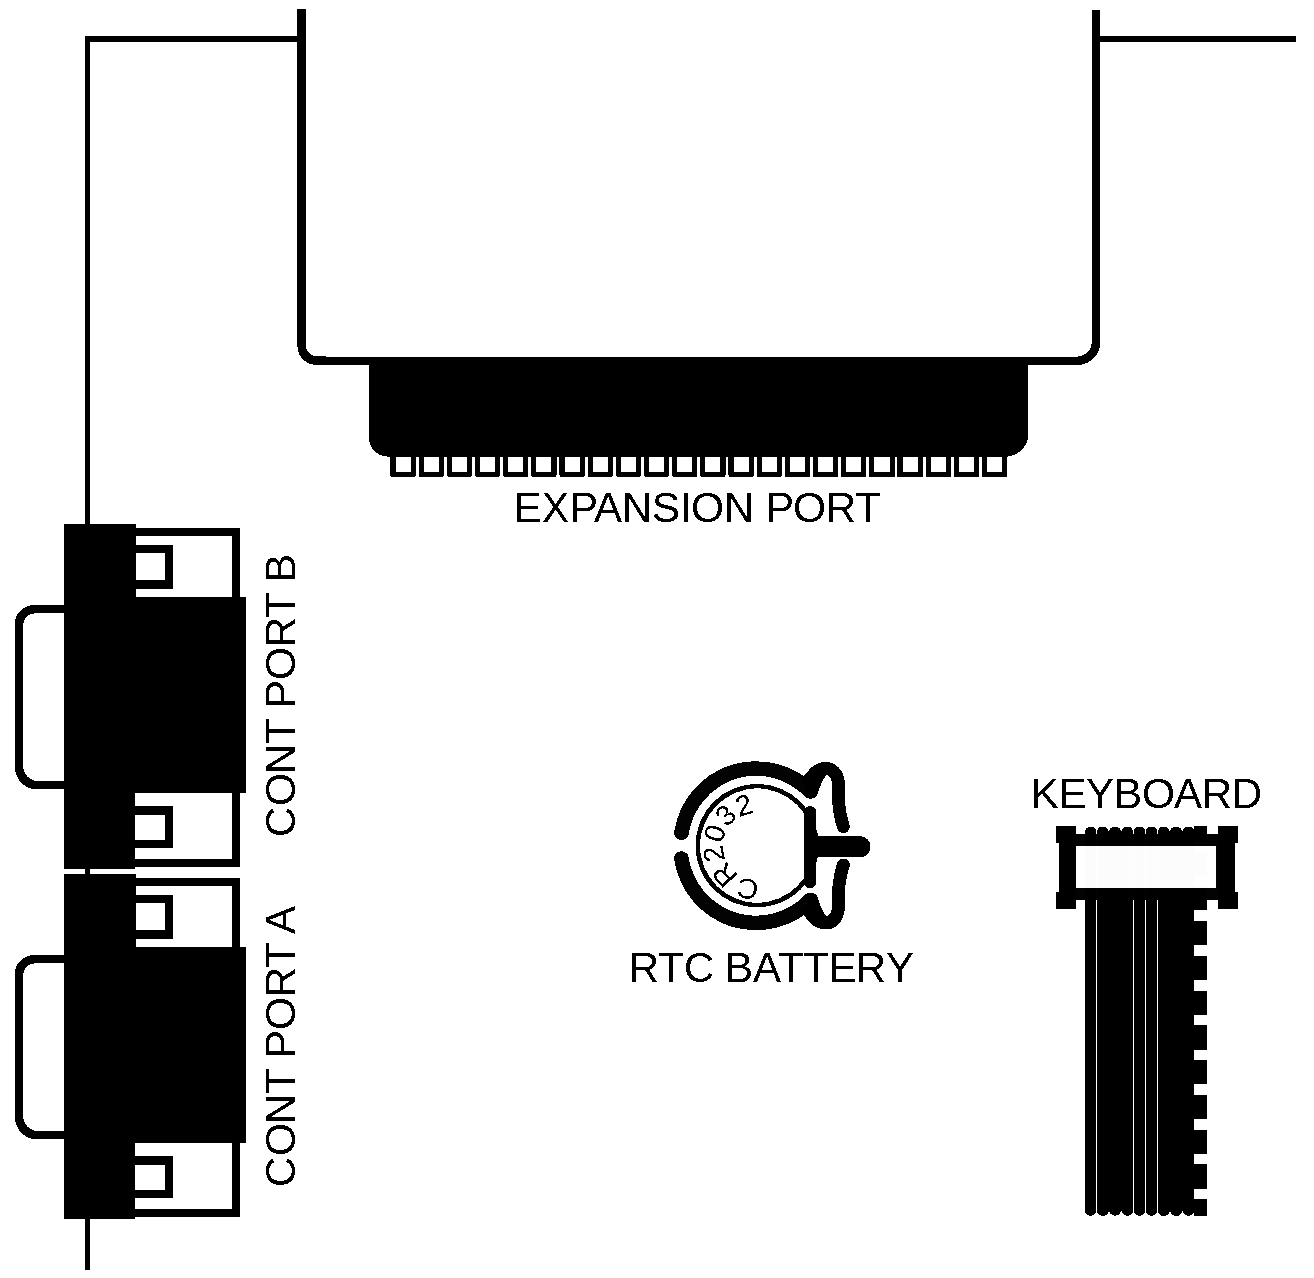
\includegraphics[width=10cm]{images/illustrations/rtc-battery-location.pdf}

If you are removing an existing battery, push the battery release lever on the bottom (flat-sided) side of the battery socket away from the battery to remove it. Insert the new battery with the side labelled {\bf +} facing up, and press it into place.

Once you have re-assembled your MEGA65, you can set the time in the Configure menu. For more information on how to set the Real-Time Clock, refer to the Configuration Utility section on page \pageref{sec:configuration-utility}.


\newpage

\section{Switching the MEGA65 on for the First Time}
\label{onboarding}

Switch the MEGA65 on using the power switch on the left-hand side of the computer.

When you switch your MEGA65 on for the first time, it displays the initial configuration (``on-boarding'') screen. You can use this screen to set the time and date on the Real-Time Clock (if you have installed the CR2032 battery), change the video display mode, and test the audio. All of these settings can be changed later.

\begin{center}
  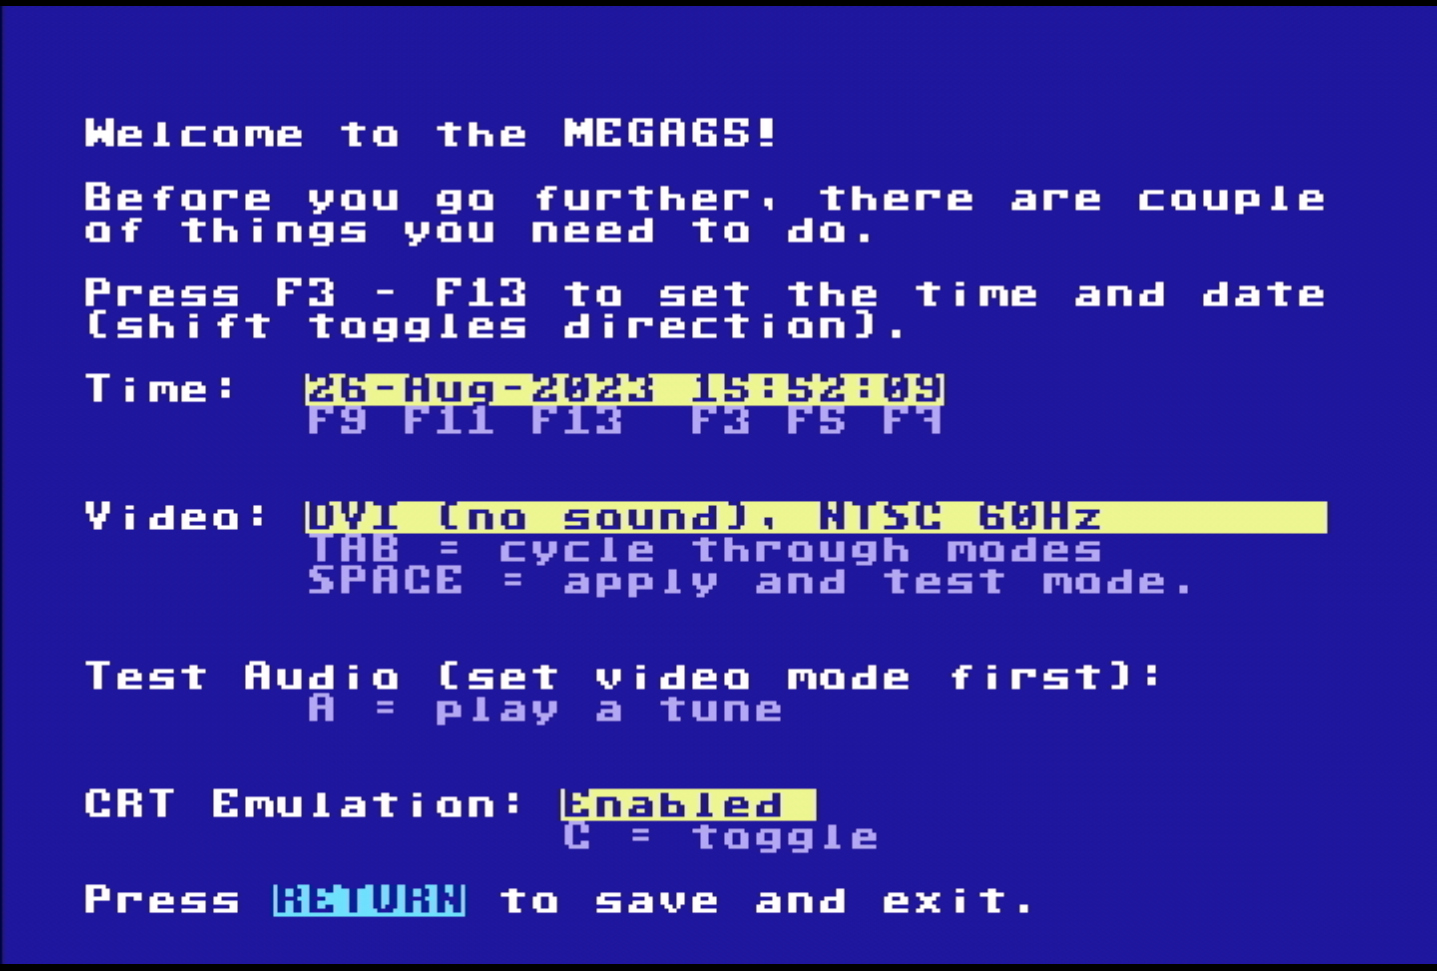
\includegraphics[trim= 10mm 15mm 10mm 10mm,clip,width=0.7\linewidth]{images/img011_final_boot_01.png}
\end{center}

For video display modes, you can select between PAL or NTSC emulation, and you can select whether your DVI display supports sound. If you are using the VGA video output, the DVI sound mode has no effect.

\underline{Note}: A DVI display that does not support sound will not work with the ``enhanced'' sound mode. With such a display, you must select a video mode with ``no sound,'' and connect a speaker to the 3.5 mm audio jack.

PAL and NTSC are analog video signal formats that affect the the resolution and vertical sync speed of the video output, even when using a modern digital display. Your display may support either mode, or it may only support one or the other. You can use this screen to test the modes with your display.

Select and test you video configuration. For example, press \specialkey{TAB} to switch to the ``PAL 50HZ'' mode.
\index{Display!Setting PAL/NTSC}
\begin{center}
  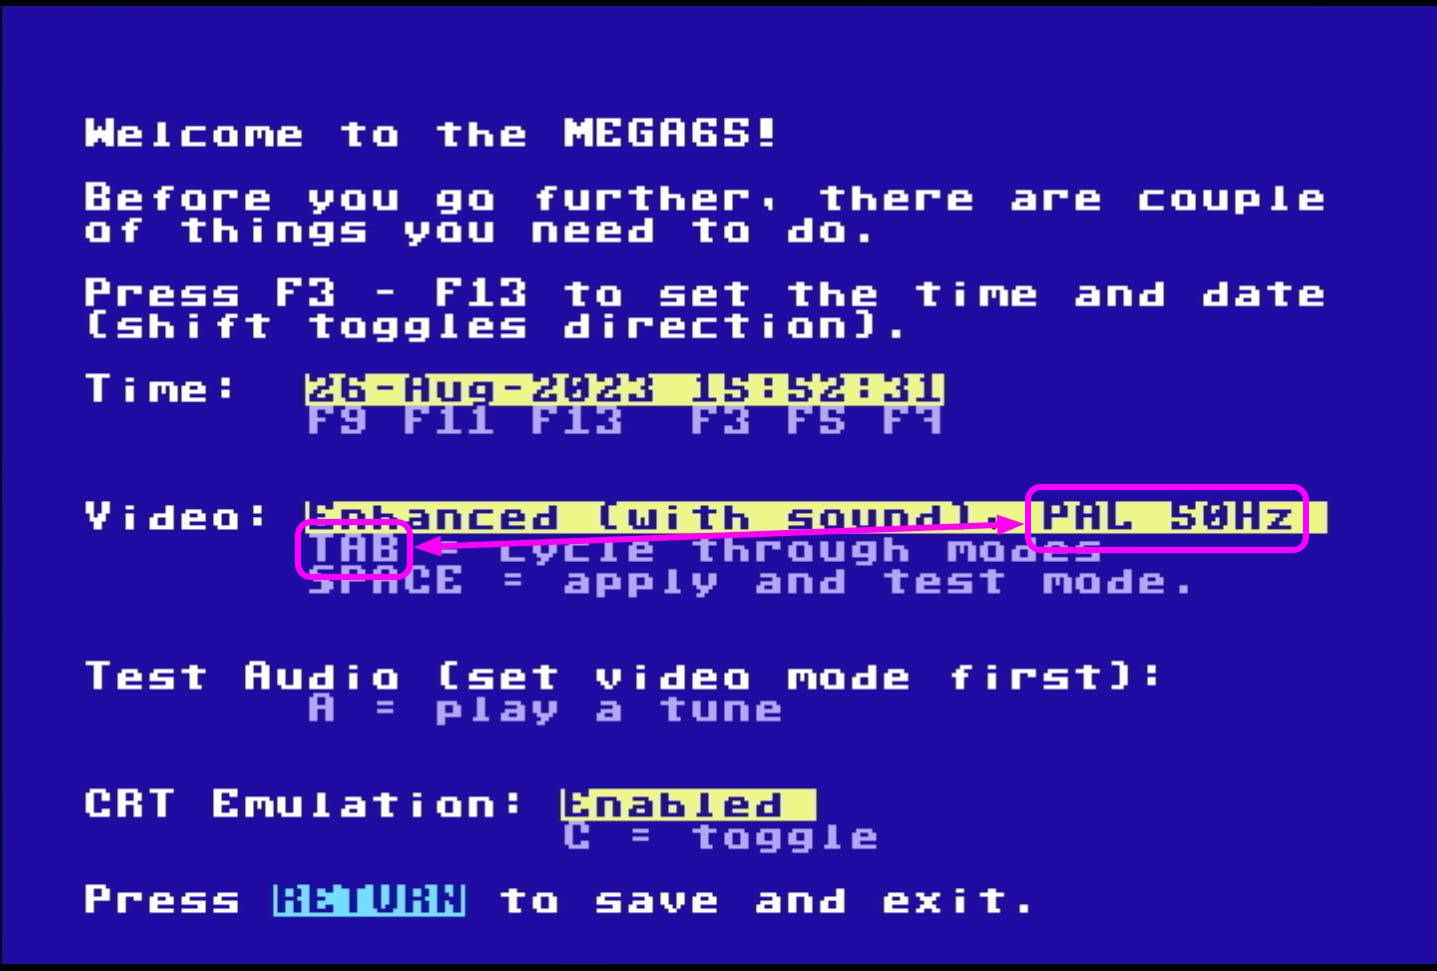
\includegraphics[width=0.7\linewidth]{images/img011_final_boot_02.png}
\end{center}

Press \megakey{SPACE} followed by \megakey{Y} to test the new video mode.

\begin{center}
  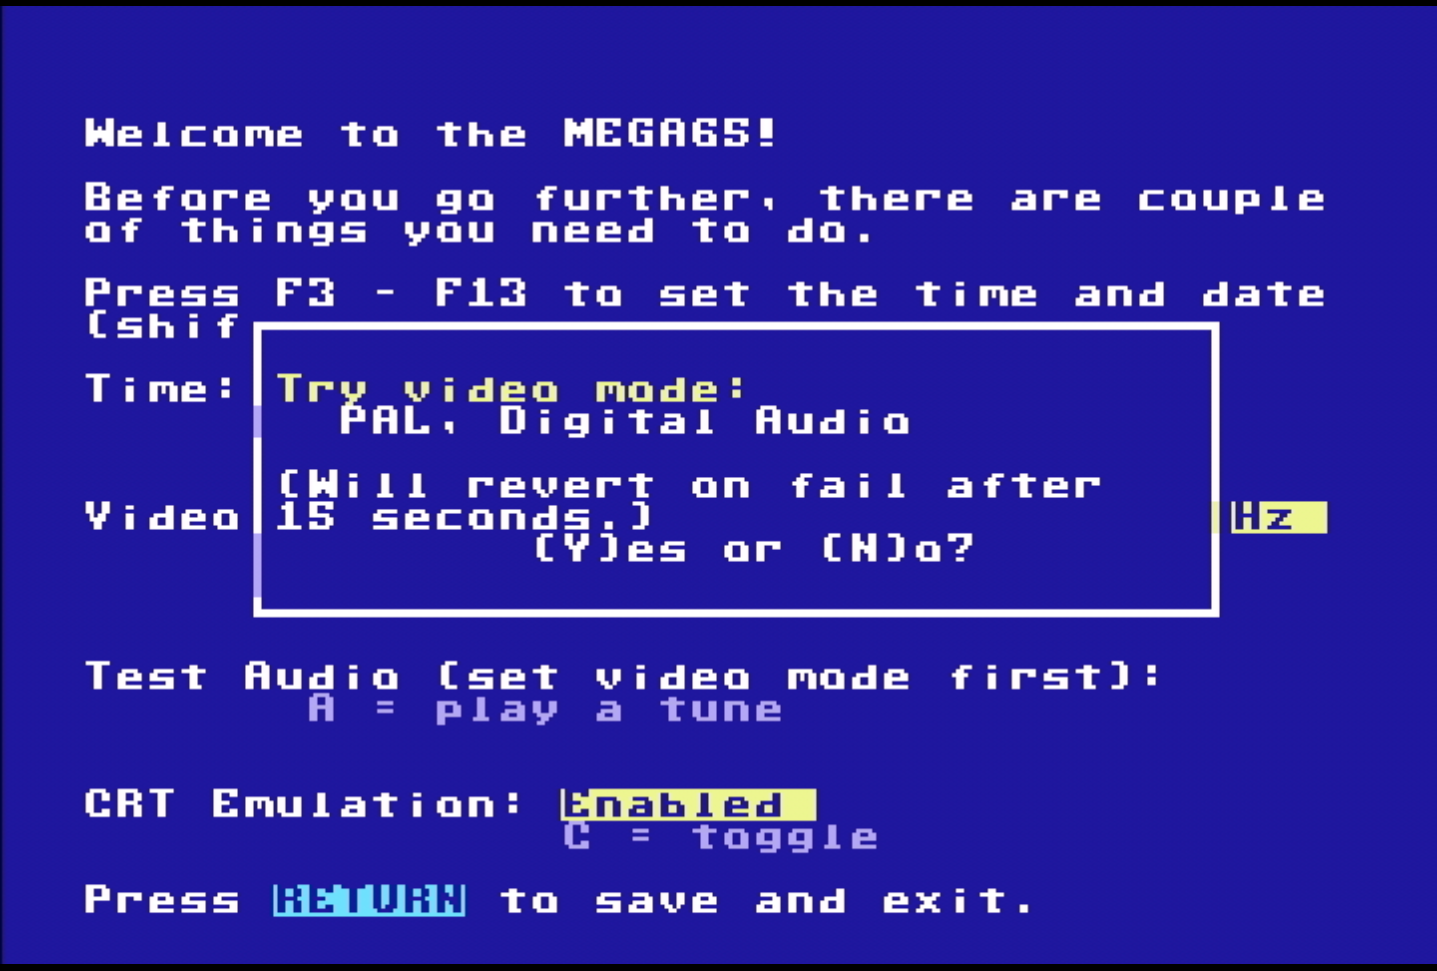
\includegraphics[trim= 15mm 10mm 10mm 15mm,clip,width=0.7\linewidth]{images/img011_final_boot_03.png}
\end{center}

Press \megakey{K} to keep the new video mode.

\begin{center}
  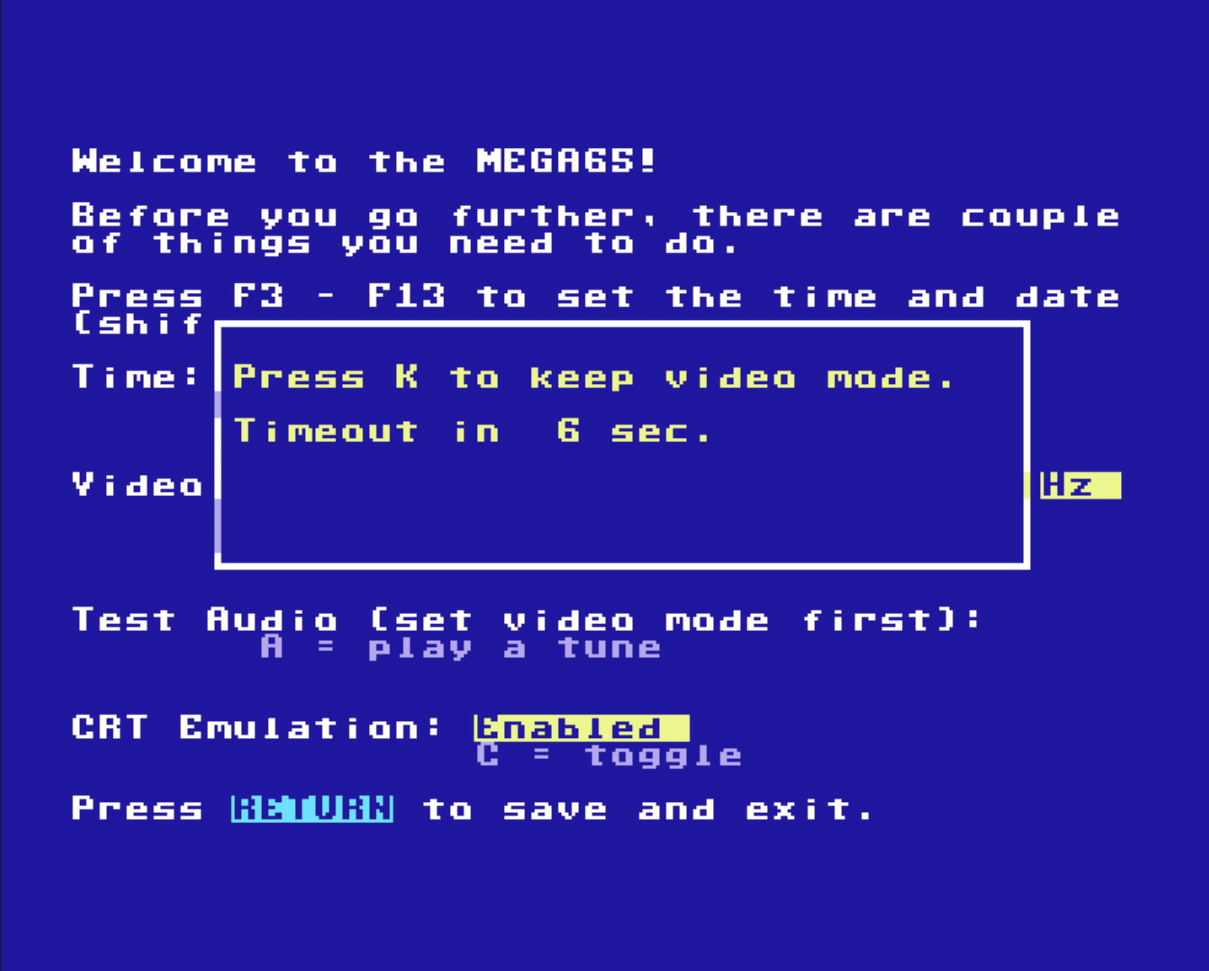
\includegraphics[trim= 20mm 20mm 10mm 25mm,clip,width=0.7\linewidth]{images/img011_final_boot_04.png}
\end{center}

Take this opportunity to test your sound set-up. Press \megakey{A} to play a sound.

The ``CRT emulation'' option is a fun choice when using a modern flat panel display. It adds vertical gaps between pixels to simulate the CRT raster line. Try it to see if you like it: press the \megakey{C} key to toggle it on and off.

Finally, press \specialkey{RETURN} to complete the configuration.

For more information about configuring your MEGA65, see chapter \vref{cha:configuringyourmega}.

\section{The Intro Disk}

After completing the on-boarding configuration, your MEGA65 starts the Intro Disk menu. The Intro Disk is a collection of software made by the MEGA65 community that demonstrates some of the capabilities of the computer. Take some time to browse the menus and try some of the demos. After each demo, press the reset button on the left-hand side of the computer to return to the Intro Disk menu.

\begin{center}
  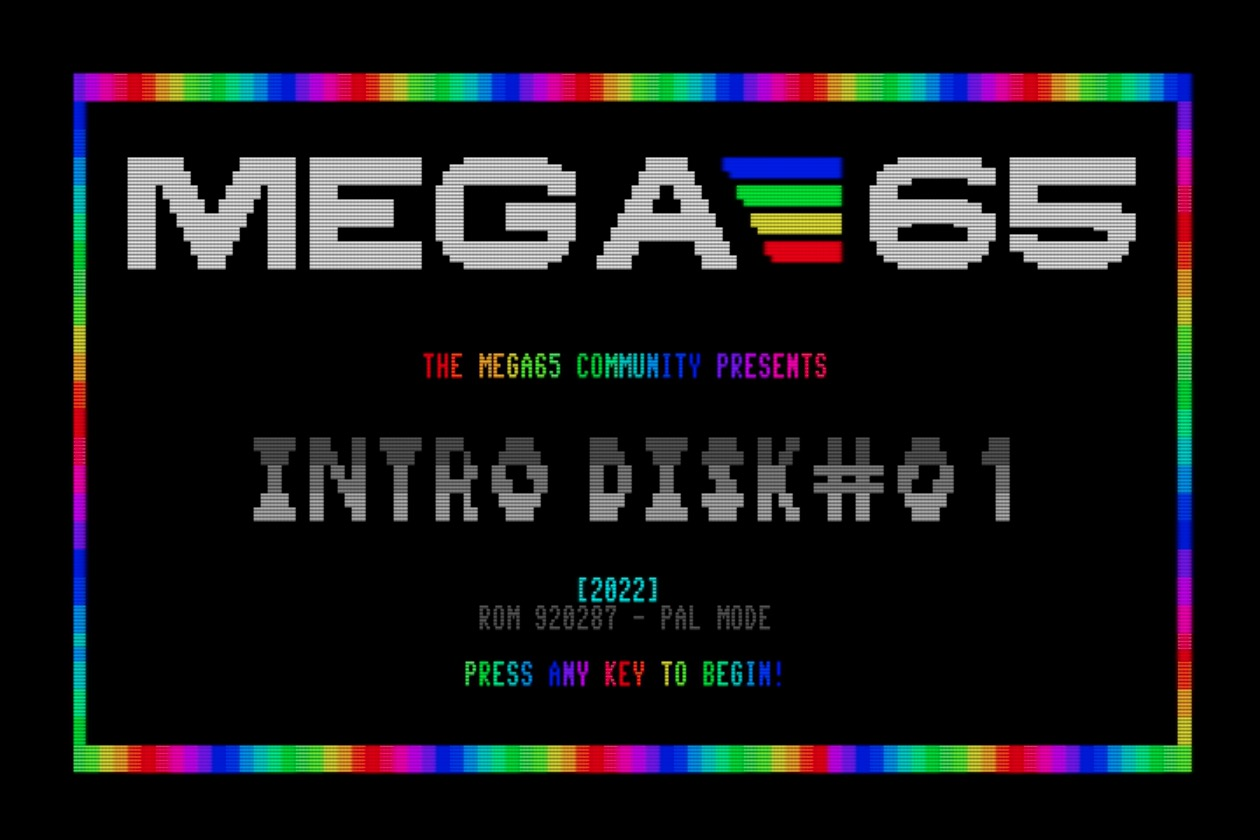
\includegraphics[width=0.7\linewidth]{images/demo_title.jpg}
\end{center}

By default, the Intro Disk menu opens each time you switch on the computer. Once you are more familiar with the MEGA65, you may wish to disable this. Press \megakey{D} at the Intro Disk menu to disable its auto-boot feature.

Press \megakey{X} to exit the Intro Disk menu and access BASIC 65. With the Intro Disk auto-boot feature disabled, the MEGA65 goes directly to BASIC 65 when you switch it on.

\begin{center}
  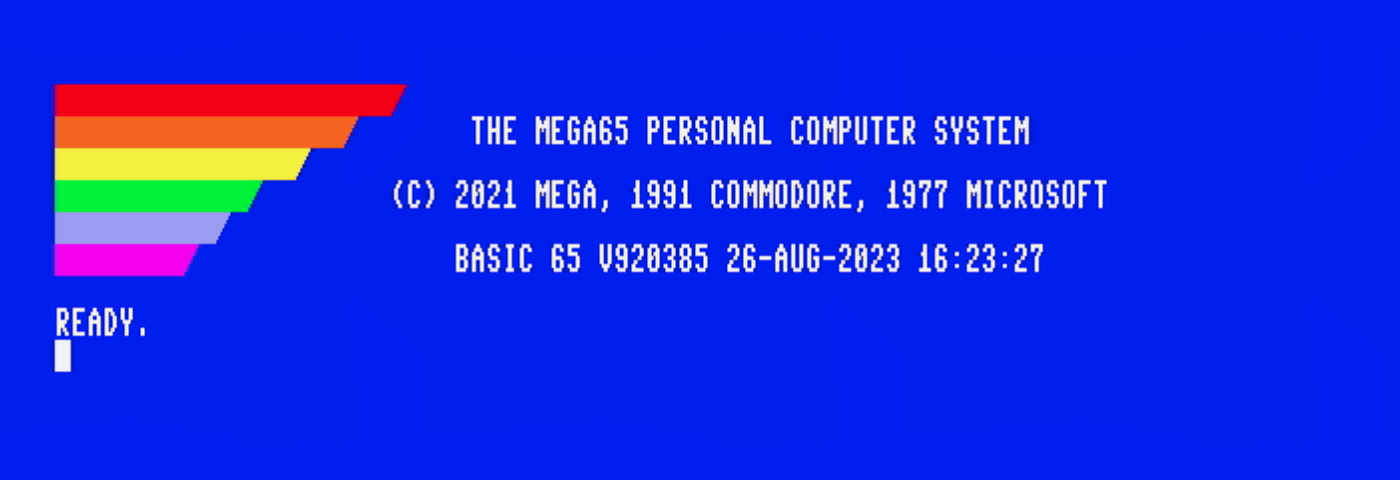
\includegraphics[trim=0 2cm 0 0,clip,width=0.7\linewidth]{images/img011_final_boot_06.png}
\end{center}

\subsection{The Cursor}

The flashing square underneath the \screentext{READY} prompt is called the cursor. The cursor indicates that the computer is ready to accept input. Pressing keys on the keyboard will print their respective characters onto the screen. The characters will be printed at the current cursor position, and the cursor will advance to the next position after every key press.

Here you can type commands, that can do things such as loading a program. You can also start entering program code!

\chapter{Getting Started}
\addtocontents{toc}{\protect\setcounter{tocdepth}{2}}
\hypersetup{bookmarksdepth=5}


\phantomsection
\section{Keyboard}
\label{cha:getting-started}

Now that everything is connected, it's time to get familiar with the MEGA65 keyboard.

You may notice that the keyboard is a little different from the keyboards used on computers today. While most keys will be in familiar positions, there are some specialised keys, and some with special graphic symbols marked on the front.

Here's a brief description of how some of these special keys function.

\subsection{Special Keys}

\subsubsection{RETURN}
\index{Keyboard!RETURN}
Pressing \specialkey{RETURN} enters the information you have typed into the MEGA65's memory. The computer will either act on a command, store some information, or display an error message if you made a mistake.

\subsubsection{SHIFT}
\index{Keyboard!Shift Keys}
The two \specialkey{SHIFT} keys are located on the left and the right. They work very much like the Shift key on a regular keyboard, however they also perform some special functions as well.

In upper case mode, holding down \specialkey{SHIFT} and pressing any key with two graphic symbols on the front produces the right-hand symbol on that key. For example, \specialkey{SHIFT} and \megakey{J} prints the \graphicsymbol{J} character.

In lower case mode, pressing \specialkey{SHIFT} and a letter key prints the upper case letter on that key.

Finally, holding \specialkey{SHIFT} down and pressing a Function key accesses the function shown on the front of that key. For example: \specialkey{SHIFT} and \megakey{F1} activates \megakey{F2}.


\subsubsection{SHIFT LOCK}
\index{Keyboard!SHIFT LOCK}
In addition to \specialkey{SHIFT} is \specialkey{SHIFT\\LOCK}. Press this key to lock down the Shift function. Now any key you press while \specialkey{SHIFT\\LOCK} is illuminated prints the character to the screen as if you were holding down \specialkey{SHIFT}. This includes special graphic characters.

\subsubsection{CTRL}
\index{Keyboard!CTRL}
\specialkey{CTRL} is the Control key. Holding down \specialkey{CTRL} and pressing another key allows you to perform Control Functions. For example, holding down \specialkey{CTRL} and one of the number keys (from \megakey{1} to \megakey{8}) allows you to change text colours. The colour that is printed at the top row on the front of the number key will be used. Holding down \specialkey{CTRL} and pressing \megakey{9} or \megakey{0} switches reverse-text mode on and off.

There are some examples of this on page \pageref{sec:screen-editor}, and all of the Control Functions are listed on page \pageref{appendix:controlcodes}.

If a program is being {\bf LIST}ed to the screen, holding down \specialkey{CTRL} slows down the display of each line. You can read
more about the {\bf LIST} command on page \pageref{basic65-list}.

Holding \specialkey{CTRL} and pressing \megakey{*} enters the Matrix Mode Debugger (refer to the {\bf MEGA65 Book} for more details).

\subsubsection{RUN STOP}
\index{Keyboard!RUN STOP}
Normally, pressing \specialkey{RUN STOP} stops the execution of a program. Holding \specialkey{SHIFT} while pressing \specialkey{RUN STOP} {\bf RUN}s the first program from disk.

Some programs override the \specialkey{RUN STOP} key and cannot be stopped in this way.

You can boot your MEGA65 into the {\bf Machine Code Monitor} by holding down \specialkey{RUN STOP} and pressing reset on the left-hand side.

\subsubsection{RESTORE}
\index{Keyboard!RESTORE}
The computer screen can be restored to a clean state without clearing the memory by holding down \specialkey{RUN STOP} and pressing \widekey{RESTORE}. This combination also resets operating system vectors and re-initialises the screen editor, which makes it a handy combination if the computer has become a little confused.

Some programs override the \specialkey{RUN STOP} or \widekey{RESTORE} key and cannot be reset in this way.

You can also enter the {\bf Freezer} by pressing and holding \widekey{RESTORE} for half to one second. You can
read more about the Freezer on page \pageref{sec:freezer}.

\newpage

\subsubsection{THE CURSOR KEYS}
\index{Keyboard!Cursor Keys}
At the bottom right-hand side of the keyboard are the cursor keys. These four directional keys allow you move the cursor to any position for on-screen editing.

The cursor moves in the direction indicated on the keys: \megakey{$\leftarrow$} \megakey{$\uparrow$} \megakey{$\rightarrow$} \megakey{$\downarrow$}.

You don't have to keep pressing a cursor key over and over. If you need to move the cursor a long way, you can keep the key pressed down. When you are finished, simply release the key.

\subsubsection{ARROW KEYS}
\index{Keyboard!Arrow Keys}
These keys are different from the cursor keys! They are \megakeywhite{$\leftarrow$} (next to \megakey{1}), and \megakeywhite{$\uparrow$} (next to \widekey{RESTORE}).
Both arrow keys are used in various BASIC functions and escape sequences.

For example, \megakeywhite{$\leftarrow$} can be used as a shortcut for {\bf SAVE}, and \megakeywhite{$\uparrow$}
is used to raise a number to a power (which is the same as multiplying a number by itself a specified number of times).

You can read more about the available escape sequences on page \pageref{escape-sequences}.

These two PETSCII specific keys will always be shown in MEGA65 literature with a white background.

\subsubsection{INSerT/DELete}
\index{Keyboard!INST DEL}
This is the INSERT / DELETE key. When pressing \specialkey{INST\\DEL}, the character to the left is deleted, and all characters to the right are shifted one position to the left.

To insert a character, hold \specialkey{SHIFT} and press \specialkey{INST\\DEL}. All the characters to the right of the cursor are shifted to the right. This allows you to type a letter, number or any other character at the newly inserted space.


\subsubsection{CLeaR/HOME}
\index{Keyboard!CLR HOME}
Pressing \specialkey{CLR\\HOME} places the cursor at the top left-most position of the screen.

Holding down \specialkey{SHIFT} and pressing \specialkey{CLR\\HOME} clears the entire screen {\it and} places the cursor at the top left-most position of the screen.

If you press \specialkey{CLR\\HOME} accidentally, you can return the cursor to its original position by pressing \specialkey{ESC} then \specialkey{CLR\\HOME}.

\subsubsection{MEGA KEY}
\index{Keyboard!MEGA Key}
\megasymbolkey or the MEGA key provides a number of different functions and can be used to launch special utilities.

Holding \specialkey{SHIFT} and pressing \megasymbolkey switches between lower and uppercase character modes.

Holding \megasymbolkey and pressing any key with two graphic symbols on the front prints the left-most graphic symbol to the screen. For example,
\megasymbolkey and \megakey{D} prints the \graphicsymbol{d} symbol.

Holding \megasymbolkey and pressing any key that shows a single graphic symbol on the front prints that graphic symbol to the screen.

Holding \megasymbolkey and pressing a number key switches to one of the colours in the second range, i.e., the colour that is printed at the bottom row on the front of the number key will be used.

Holding \megasymbolkey and pressing \specialkey{TAB} enters the Matrix Mode Debugger (refer to the {\bf MEGA65 Book} for more details).

Switching on the MEGA65 or pressing the reset button on the left-hand side while holding down \megasymbolkey switches the MEGA65 into C64-mode.

\subsubsection{NO SCROLL}
\index{Keyboard!NO SCROLL}
If a program is being {\bf LIST}ed to the screen, pressing \specialkey{NO\\SCROLL} pauses the screen output. Press any key to un-pause.

This feature is not available in C64-mode.

\subsubsection{Function Keys}
\index{Keyboard!Function Keys}
There are seven Function keys available for use by software applications. \megakey{F1} \megakey{F3} \megakey{F5} \megakey{F7} \megakey{F9} \megakey{F11} and \megakey{F13} can be used to perform special functions.

Hold \specialkey{SHIFT} to access \megakey{F2} through to \megakey{F14} as shown on the front of each Function key.
\index{Keyboard!Shift Keys}
Only Function keys \megakey{F1} to \megakey{F8} are available in C64-mode.

\subsubsection{HELP}
\index{Keyboard!HELP}
\specialkey{HELP} can be used by software and also acts as \megakey{F15} / \megakey{F16}.

\subsubsection{ALT}
\index{Keyboard!ALT}
Holding \specialkey{ALT} down while pressing other keys can be used by software to perform specific functions. Not available in C64-mode.

Holding \specialkey{ALT} down while switching the MEGA65 on activates the Utility Menu. You can format an SD card, or enter the MEGA65 Configuration Utility to select the default video mode and change other settings, or to test your keyboard.

\subsubsection{CAPS LOCK}
\index{Keyboard!CAPS LOCK}
\specialkey{CAPS\\LOCK} works similarly to \specialkey{SHIFT\\LOCK} in C65 and MEGA65-modes, but only modifies the letter keys.

When the MEGA65 is set to run at a reduced processor speed, such as in C64-mode, you can hold \specialkey{CAPS\\LOCK} to run the processor at full speed temporarily. This is useful in C64-mode for things such as
speeding up loading from the internal disk drive or SD card, or to greatly speeding up the de-packing process after a program is run. MEGA65 mode runs at maximum speed by default.

\addtocontents{toc}{\protect\setcounter{tocdepth}{5}}


\section{The Screen Editor}
\label{sec:screen-editor}

When you switch on your MEGA65 or reset it, the following screen will appear:

\begin{center}
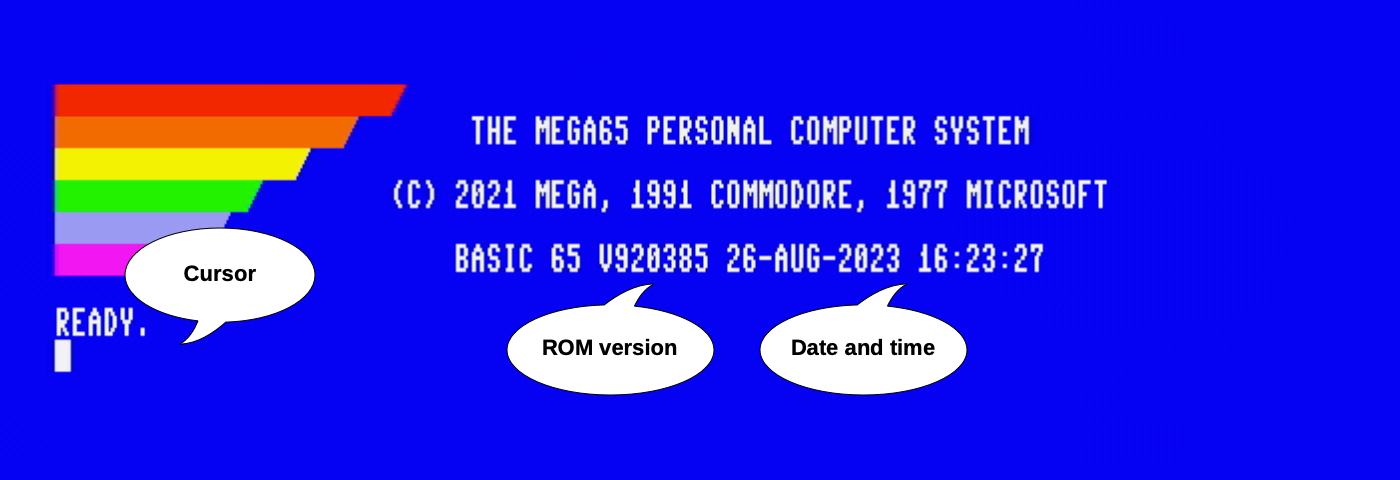
\includegraphics[width={10cm}]{images/introduction-screen/layout.png}
\end{center}

The colour bars in the top left-hand side of the screen can be used as a guide to help calibrate the colours of your display. The screen also displays the name of the system, the copyright notice, and the ROM version. The displayed date and time are taken from the internal RTC (Real-Time Clock) at the time the computer was powered on. You can set the date and time in the Configure Menu.

Finally, you will see the \screentext{READY} prompt and the flashing cursor.

You can begin typing keys on the keyboard and the characters will be
printed at the cursor position. The cursor itself will advance after
each key press.

You can also produce reverse text or colour bars by holding down \specialkey{CTRL} and pressing \megakey{9}, or \megakey{R}. This enters reverse text mode. When this is enabled, you can press and hold the \megakey{Space} bar. While doing so, a white bar will be drawn across the screen.
\index{Keyboard!CTRL}
You can even change the current colour by holding \specialkey{CTRL} down and pressing a number key (from \megakey{1}
to \megakey{8}). For example, if you press and hold \specialkey{CTRL} down and press \megakey{1}, the colour will
change to black. Now, when you hold down the \megakey{Space} bar, a black bar will be drawn. If you continue to
change the colour and press the \megakey{Space} bar, you will get an effect similar to the following image:

\begin{center}
\includegraphics[width={10cm}]{images/introduction-screen/colour-bars.png}
\end{center}

\index{Keyboard!MEGA Key}
You can disable reverse text mode by holding \specialkey{CTRL} and pressing \megakey{0}.

By pressing any key, characters will be printed to the screen in the chosen colour.

A further eight colours can be selected by holding down \megasymbolkey and pressing a key from \megakey{1} to \megakey{8}.
The colour that is printed at the bottom row on the front of the number key will be used. For example, if you held
\megasymbolkey down while pressing \megakey{4}, dark grey will be used. For access to an additional 16 colours of the alternate/rainbow palette, refer to the \specialkey{CTRL} + \megakey{A} shortcut described on page \pageref{appendix:controlcodes}.

\underline{Note}:
\begin{itemize}
  \item {\bf Quote Mode}: If you were to press \megakey{"} to open a string, and then try to change
colours, reverse text, move the cursor keys, or use the \specialkey{CLR HOME} key, instead
of these actions instantly occurring, funny PETSCII symbols will appear instead. This is
due to a BASIC facility called {\it quote mode} (described further in the \textbf{MEGA65 Book}),
which allows you to encode such actions into a string so that they can be executed at a later
time (for example, via a {\bf PRINT} statement within your programs). To end {\it quote mode}, simply
type another \megakey{"} to mark the end of your string.
  \item {\bf Insert Mode}: A similar facility is called
{\it insert mode}, where for the number of times you press \specialkey{SHIFT} + \specialkey{INST\\DEL}
to insert a few spaces, the same number of keypresses that follow it will abide by the same
principles of {\it quote mode}.
  \item You can forcefully exit either of these modes by pressing \specialkey{ESC}, \megakey{O}.
\end{itemize}

\needspace{4cm}
You can create fun pictures just by using these colours and letters.  Here's an example of what a student drew:

\begin{center}
\includegraphics[width={6cm}]{images/caleb-PETSCII-TNT-final}
\end{center}

What will you draw?

\needspace{2cm}
\textbf{Functions}

Functions using \specialkey{CTRL} are called \textbf{Control Codes}.
Functions using \megasymbolkey are called \textbf{Mega Codes}. There are also functions that are called by using \specialkey{SHIFT}, which
are called \textbf{Shifted Codes}.

Lastly, \specialkey{ESC} enables the use of \textbf{Escape Sequences}.

You can read about all of these functions in detail on page \pageref{appendix:controlcodes}.

\needspace{2cm}
\textbf{ESC Sequences}

\index{Keyboard!Escape Sequences}
Escape sequences are performed a little differently than a Control function or a Shift function. Instead of holding the modifier key down, an Escape sequence is performed by pressing \specialkey{ESC} and releasing it, followed by pressing the desired key.

For example: to switch between 40/80 column mode, press and release \specialkey{ESC}, then press \megakey{X}.

There are more modes available. You can create flashing text by holding \specialkey{CTRL} down and pressing \megakey{O}. Any characters you type in will flash. Turn flash mode off by pressing \specialkey{ESC},  then \megakey{O}.


\section{Editor Functionality}

The MEGA65 screen can allow you to do advanced tabbing, and quickly move around the screen in many ways to help you to be more productive.

For example, press \specialkey{CLR HOME} to go to the home position on the screen. Hold \specialkey{CTRL} down and press \megakey{W} several times. This is the \textbf{Word Advance function}, which jumps your cursor to the next word, or printable character.

You can set custom tab positions on the screen for your convenience. Press \specialkey{CLR HOME} and then \megakey{$\rightarrow$} to move the cursor to the fourth column. Hold down \specialkey{CTRL} and press \megakey{X} to set a tab. Move another 16 positions to the right, and press \specialkey{CTRL} and \megakey{X} again to set a second tab.

Press \specialkey{CLR HOME} to go back to the home position. Hold \specialkey{CTRL} down and press \megakey{I}. This is the \textbf{Forward Tab function}. Your cursor will tab to the fourth position. Press \specialkey{CTRL} and \megakey{I} again. Your cursor will move to position 8. By default, every 8th position is already set as a tabbed position. So the 4th and 20th positions have been added to the existing tab positions. You can continue to press \specialkey{CTRL} and \megakey{I} to advance to the 16th and 20th positions.

\subsection{Creating a Window}
\index{Keyboard!Escape Sequences}

You can set a window on the MEGA65 working screen. Move your cursor to the beginning of the "BASIC 65" text. Press \specialkey{ESC}, then press \megakey{T}. Move the cursor 10 lines down and 15 to the right.

Press \specialkey{ESC}, then \megakey{B}. Anything you type will be contained within this window.

For example, if you were to type \screentext{LIST} to list out a program, the listing will be confined to the window region you have specified:

\begin{center}
\includegraphics[width={7cm}]{images/set-window.png}
\end{center}

To escape from the window back to the full screen, press \specialkey{CLR HOME} twice.

\subsection{Additional ASCII characters}

You may have noticed a few ASCII characters on the MEGA65 keyboard that aren't traditionally a part of the PETSCII character set. In order to make use of these from within BASIC:

\begin{itemize}
  \item Type either \screentext{FONT A} or \screentext{FONT B}.
  \item Press \megasymbolkey + \specialkey{SHIFT} to switch to lowercase.
\end{itemize}

You will now be able to type those additional ASCII characters via the keyboard. To revert back to the original PETSCII character set, type \screentext{FONT C}.

\subsection{Uppercase and lowercase}

\megasymbolkey + \specialkey{SHIFT} switches between uppercase and lowercase text for the entire display. This works even during program execution, so you can adjust it if a program is in the wrong mode.


\section{The Freezer Menu}
\label{sec:freezer}

The MEGA65 spends most of its time behaving as a Commodore 65 computer would, either running a program or awaiting instructions in the BASIC environment. Your MEGA65 has additional features that were not part of the original C65 design. You can access many of these features from the Freeze menu.

To open the Freezer menu, hold the \widekey{RESTORE} key for one second, then release it. The MEGA65 will pause whatever it is doing, flicker the border color, then open the Freezer menu. Whatever program was running remains in memory and can be resumed by pressing the \specialkey{F3} key. You can also abandon the running program and reset the MEGA65 by pressing \specialkey{F5}.

\begin{center}
  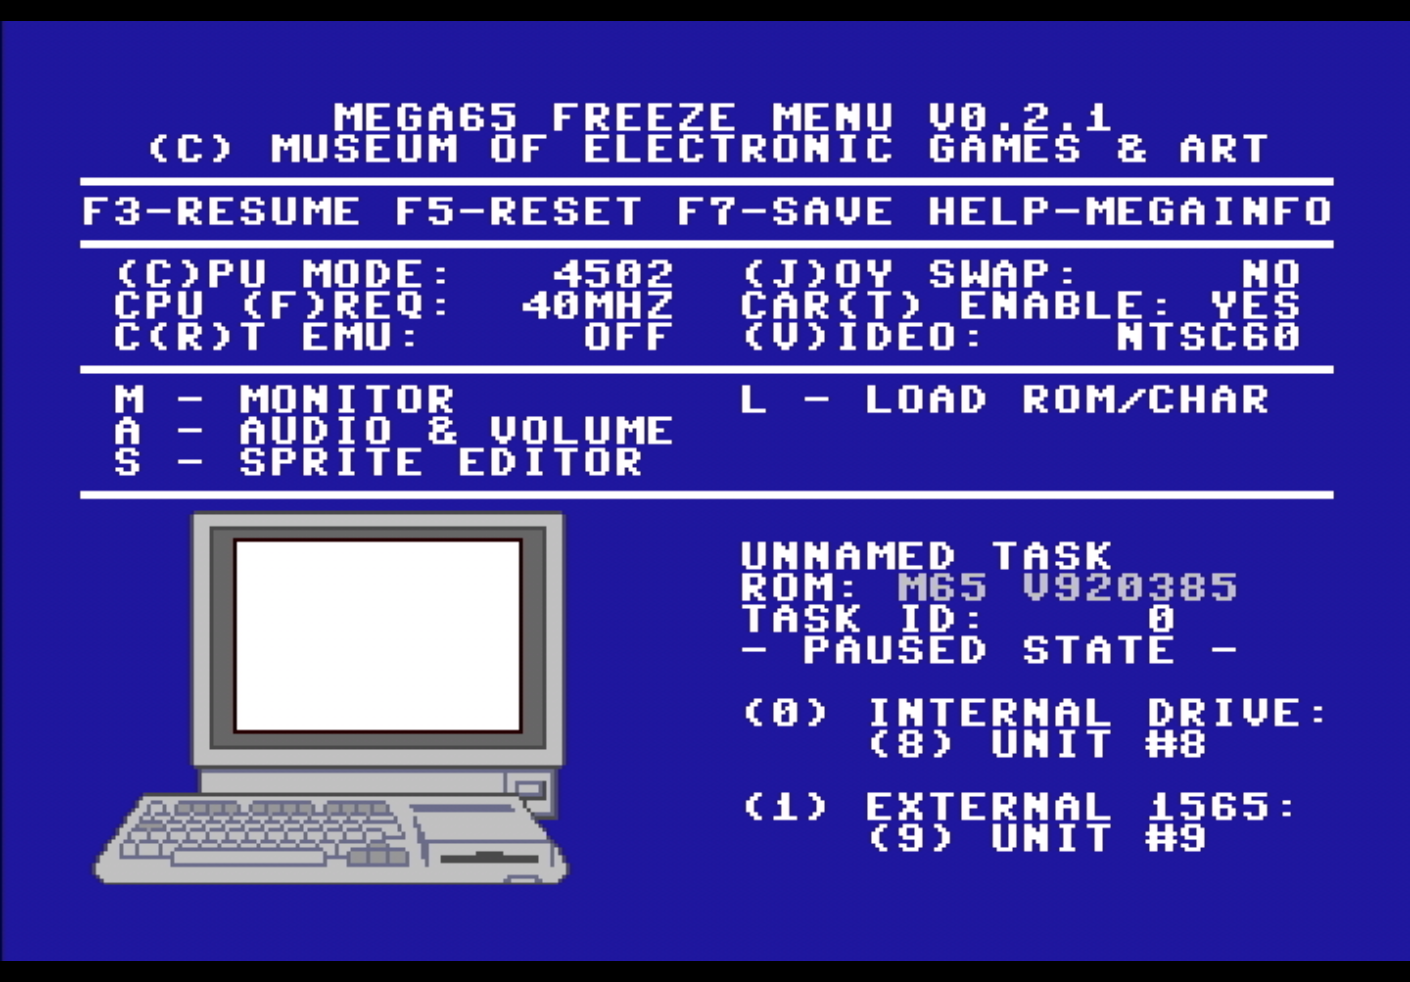
\includegraphics[width=0.7\linewidth]{images/freezer.png}
\end{center}

One feature to remember when playing games is the ``(J)OY SWAP.'' This causes the two joystick ports to trade numbers. If you have a joystick in port 2 and you start a game that expects a joystick in port 1, instead of disconnecting and reconnecting the joystick, open the Freeze menu, press \megakey{J} to swap the port numbers, then resume your game.

This is called the ``Freezer'' menu because the state of the MEGA65 remains frozen while using it. The Freezer menu can store multiple freeze states, and you can switch between them. To save the current state, navigate to an unused {\it freeze slot} using the cursor-right key, then press \megakey{F7}. When the border stops blinking, the state is saved. To restore a state, navigate to the freeze slot, then press \megakey{F3} to resume operation.

The Freezer menu has several built-in options and features. For more information about MEGAINFO, see ``Determining the Versions of Things'' on page \pageref{sec:versions}. For more information about mounting disks and disk images, see chapter \vref{cha:using-disks}.


\section{Running Commodore 64 Software}

The MEGA65 is capable of running Commodore 64 software. There are two ways to do this: the built-in GO64 mode, and the {\it C64 for MEGA65} FPGA core.

\subsection{GO64 Mode}

The original Commodore 65 was designed to be capable of running some Commodore 64 software. The MEGA65 supports this feature, known as ``GO64 mode.''

\underline{Note}: Due to how Commodore designed this feature, not all C64 software is compatible with this mode. Unlike the similar feature of the Commodore 128, the Commodore 65 uses a different CPU, and minor differences are known to be incompatible with some software titles.

There are three ways to switch the MEGA65 into GO64 mode:

\begin{itemize}
    \item Switch off the computer, hold the \megasymbolkey and switch it back on.
    \item From the MEGA65 \screentext{READY} prompt, enter this command: \screentext{GO64} Enter \screentext{YES} when prompted.
    \item Switch off the computer, connect a Commodore 64 cartridge to the expansion port, then switch the computer on.
\end{itemize}

\begin{center}
  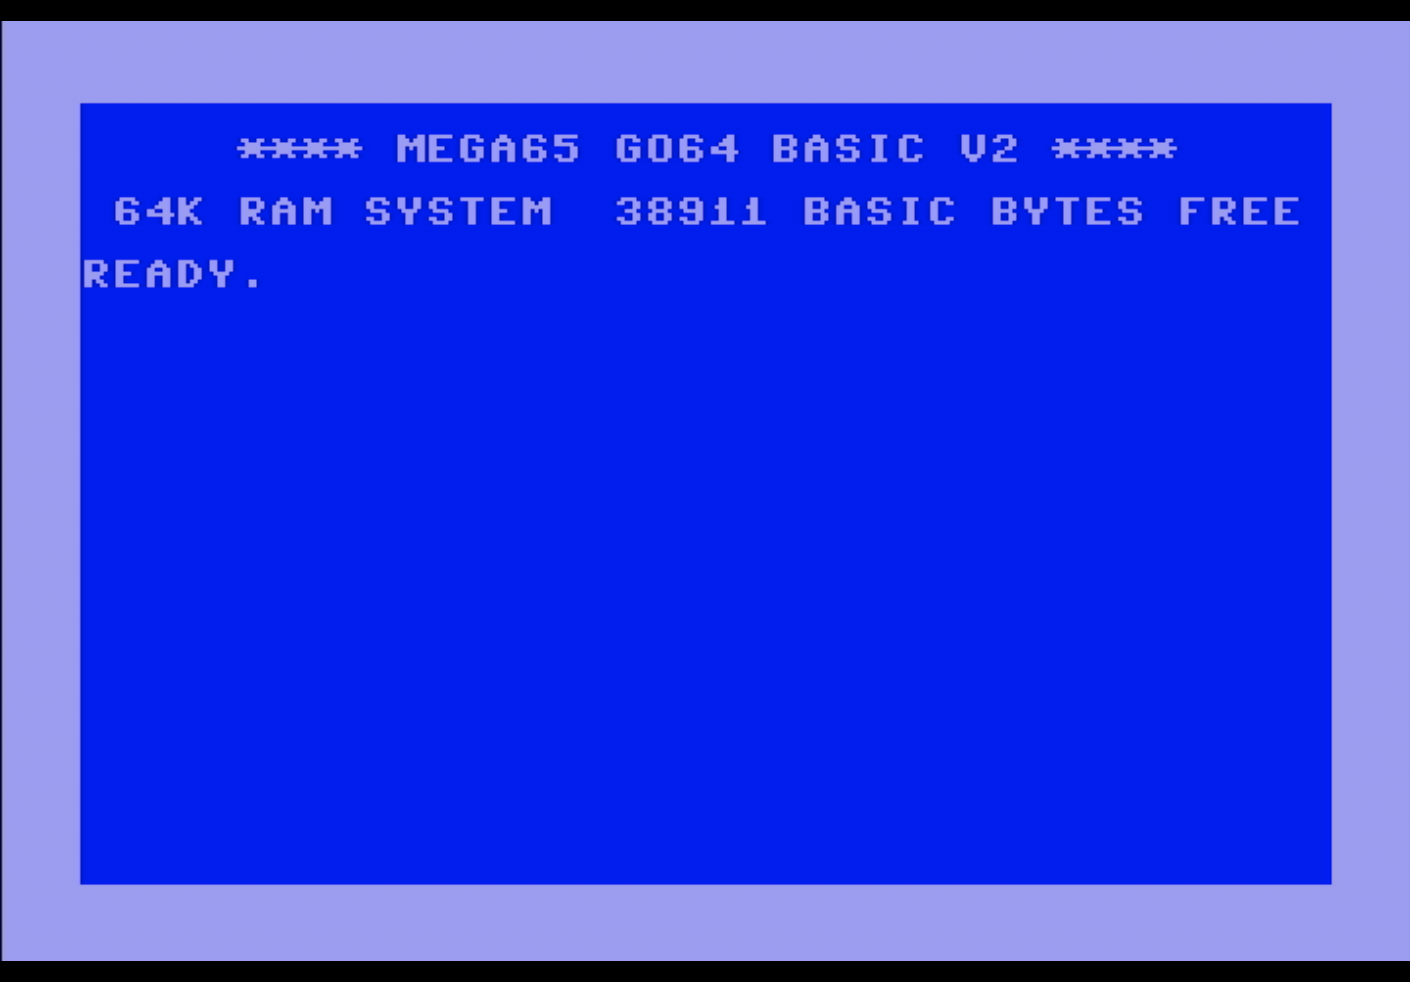
\includegraphics[width=0.7\linewidth]{images/go64.png}
\end{center}

GO64 mode is actually just a temporary re-configuration of the MEGA65. All of the MEGA65's features are still present, including the Freezer menu for mounting D81 disk images.

Much Commodore 64 software can be found on the Internet in the form of D64 disk images. The MEGA65 only supports D81 disk images via the SD card and Freezer menu. You can use a peripheral such as the SD2IEC with the MEGA65's IEC port to use D64 disk images. Be sure to obtain an SD2IEC with an independent power supply, and not one that depends on a Commodore 64 tape connector. For information on how to obtain an SD2IEC device, see: \url{https://www.thefuturewas8bit.com/sd2iec-info}

\subsection{The C64 for MEGA65 FPGA Core}

The {\it C64 for MEGA65} FPGA core by MJoergen and sy2002 re-creates the original Commodore 64 computer on MEGA65 hardware with a high degree of accuracy. It does so by completely replacing the MEGA65 core with one that implements the Commodore 64 chipset, including its CPU. MEGA65 features such as the Freezer menu are not available when running the C64 core. Instead, the core provides its own menu for mounting D64 disk images and other features. Press the \specialkey{HELP} key with the core running to access this menu.

% TODO: When the cartridge-to-core configuration feature is complete:
% With the C64 core installed, you can configure the MEGA65 boot process to use the core when a Commodore 64 cartridge is connected, instead of using the less-compatible GO64 mode. ...

For information about installing FPGA cores, see chapter \vref{cha:cores}. To download the {\it C64 for MEGA65} core and read important installation instructions, see: \url{https://github.com/MJoergen/C64MEGA65}

\chapter{Configuring Your MEGA65}
\label{cha:configuringyourmega}

\section{Configuring Your MEGA65}

This chapter describes how to configure your MEGA65.

Configuration data is stored on the SD card, so this chapter also describes how to prepare a new SD card. Your MEGA65 comes with an SD card pre-installed. If you configure your MEGA65 using the pre-installed SD card then later install a new SD or microSD card, you will need to set your configuration settings again.

This chapter also introduces the MEGA65 Filehost website, which you can use to download games, apps, tools, and system updates for your computer.

\section{The Configuration Utility}
\label{sec:configuration-utility}

You can configure your MEGA65 using the Configuration Utility. This includes the settings shown when you switched on the machine for the first time, and many others.

To access the Configuration Utility, switch off the MEGA65, hold the \megakey{ALT} key and switch it back on. The utility menu appears with several options. Press \megakey{1} to start the Configuration Utility.

\begin{center}
  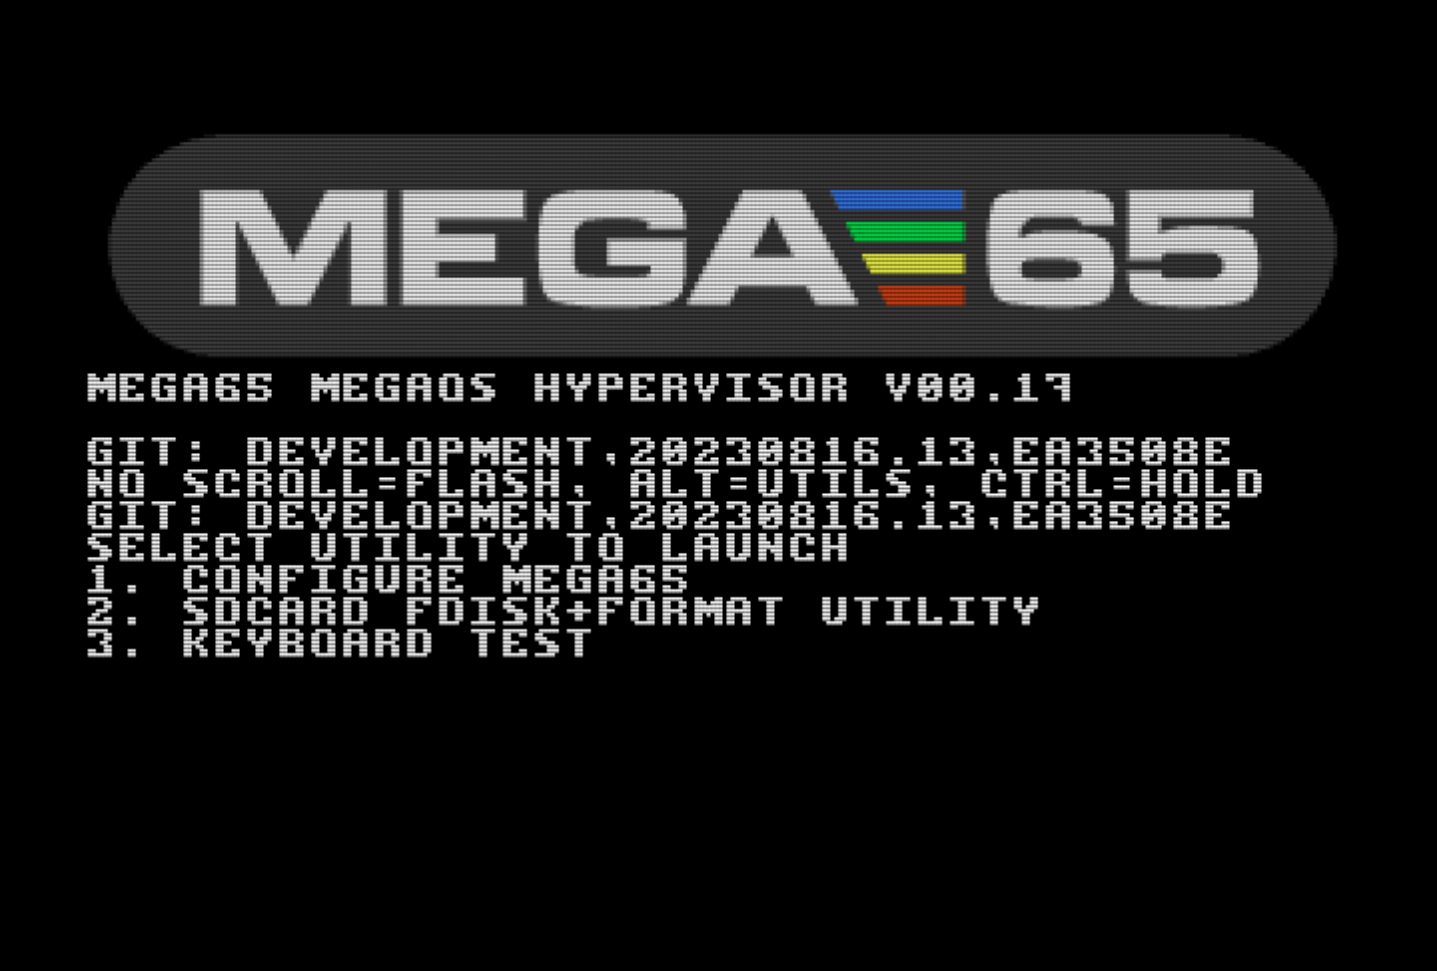
\includegraphics[width=0.7\linewidth]{images/ss-utilmenu.png}
\end{center}

The Configuration Utility includes several pages of settings, which you can navigate using the keyboard or a mouse connected to port 1. Use \megakey{$\leftarrow$} and \megakey{$\rightarrow$} to navigate between pages, and \megakey{$\uparrow$} and \megakey{$\downarrow$} to select items on the page. Press \specialkey{RETURN} or \megakey{SPACE} to toggle a setting or change a value.

\subsection{Input}

The ``Input'' page configures the mouse settings for the two peripheral ports.

\begin{center}
  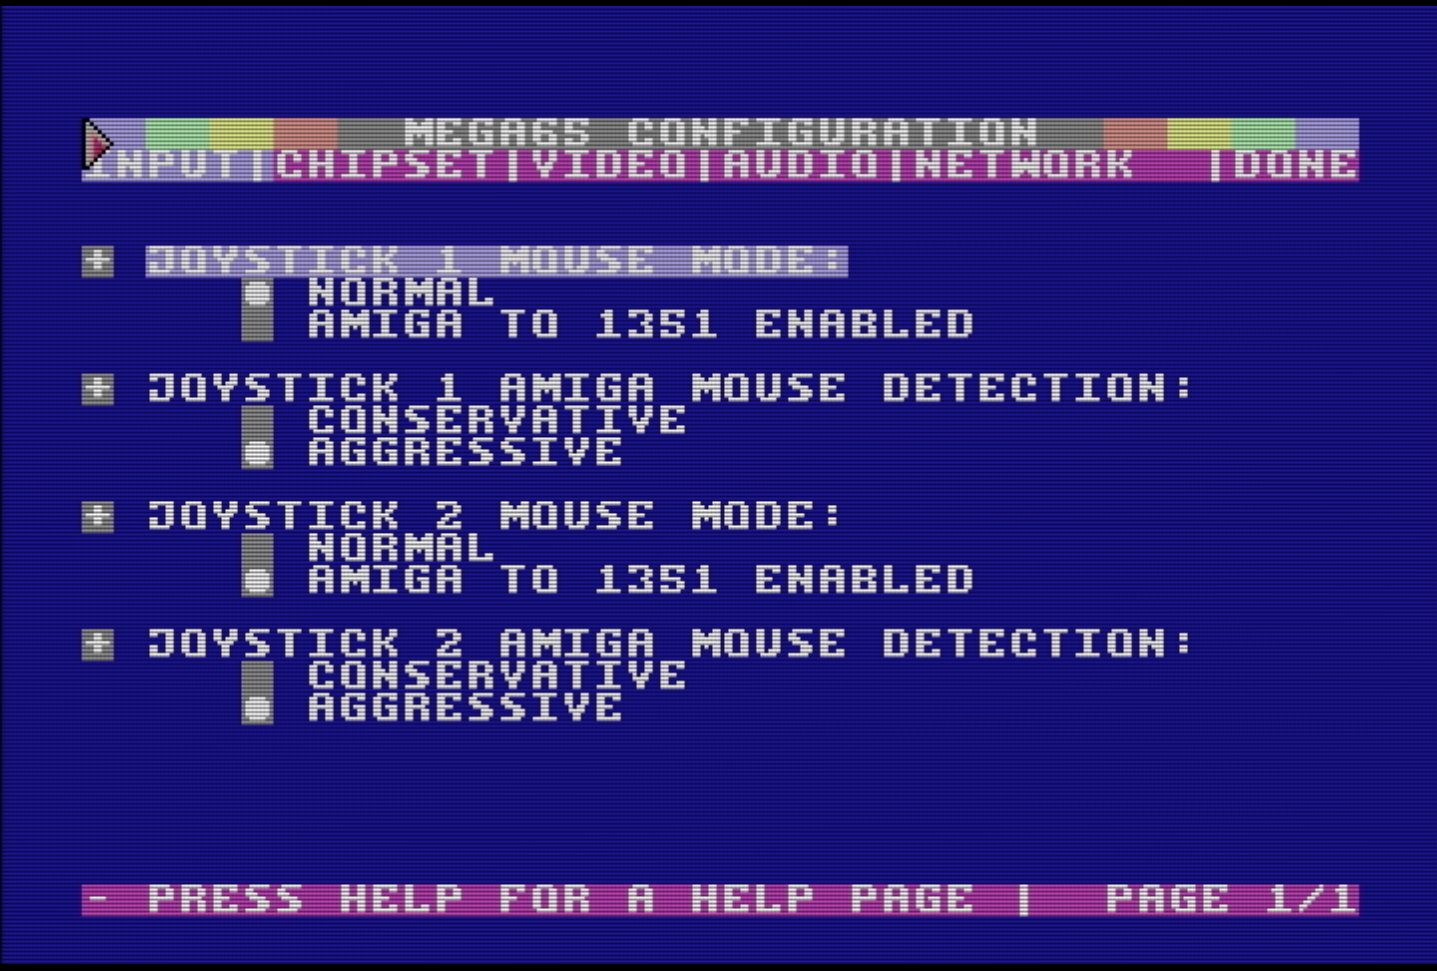
\includegraphics[width=0.7\linewidth]{images/ss-m65config-1.png}
\end{center}

The MEGA65 supports the Commodore 1351 mouse, the Commodore Amiga mouse, or modern equivalents such as a USB mouse connected with a \href{https://retrohax.net/shop/amiga/mouster/}{mouSTer} adapter. The port must be set to the correct mouse type, where ``normal'' refers to the 1351 mouse. If an Amiga mouse is connected while the port is in the ``normal'' mode, it may interfere with the behavior of the keyboard.

``Amiga mouse detection'' controls how the MEGA65 interprets Amiga mouse signals and converts them to equivalent 1351 signals. Some joysticks experience interference on a port with Amiga mouse mode enabled. If you notice any such interference, change this setting to ``conservative,'' otherwise leave it set to ``aggressive.''

\subsection{Chipset}

The ``Chipset'' page configures several features, including the Real-Time Clock.

\begin{center}
  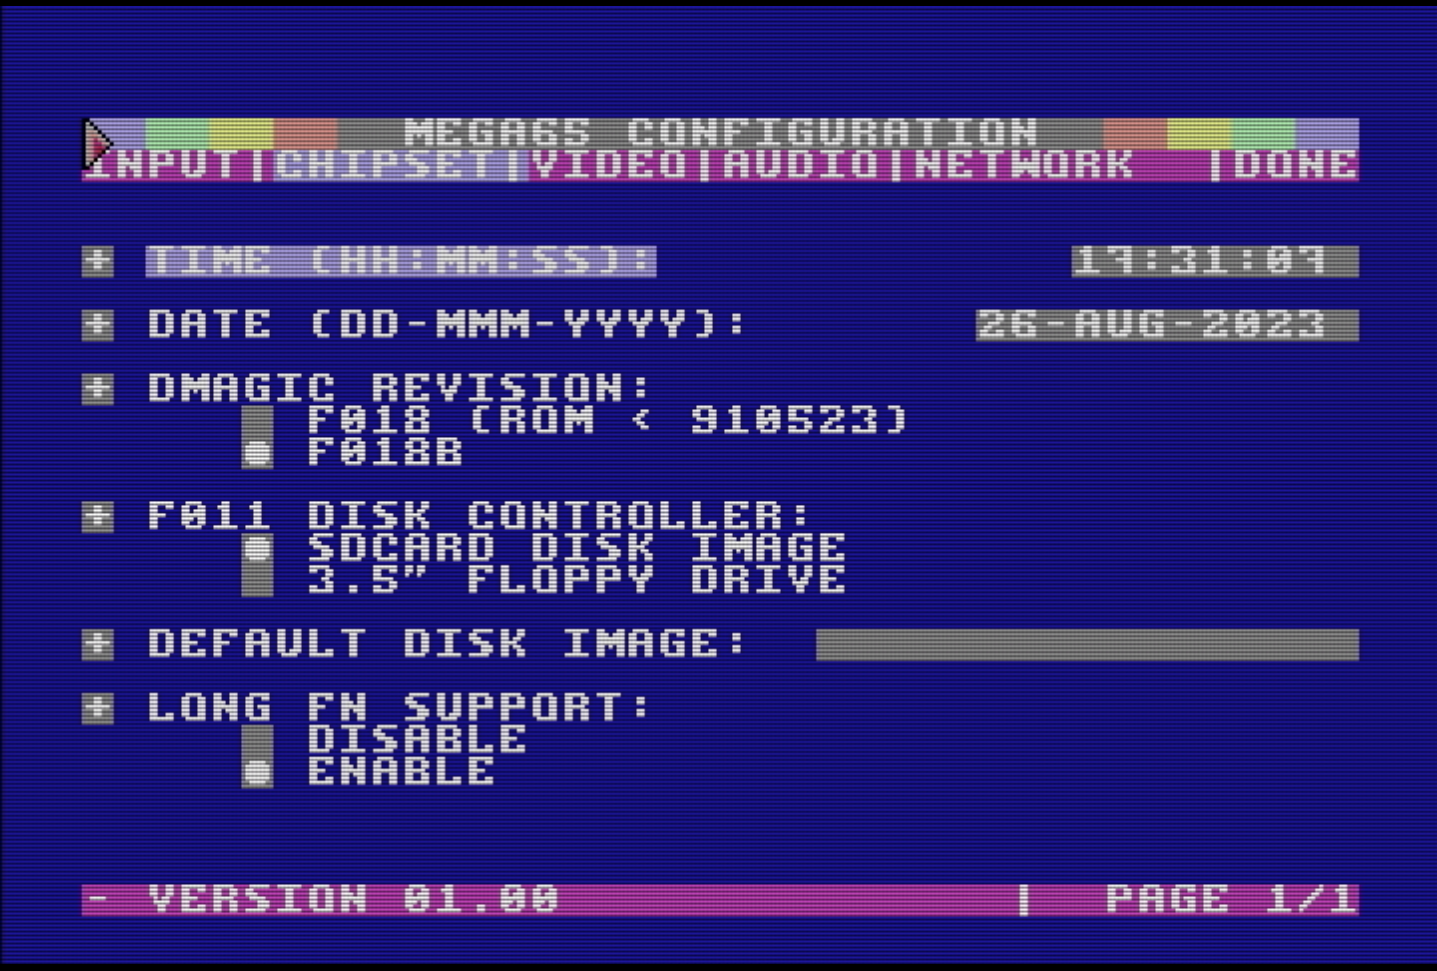
\includegraphics[width=0.7\linewidth]{images/ss-m65config-2.png}
\end{center}

To set the Real-Time Clock, select the time or date field, type the complete value, then press \specialkey{RETURN}. The clock setting takes effect as soon as you press \specialkey{RETURN}, and does not take effect unless you press \specialkey{RETURN}. Note that all other settings are not saved until the end. Only the RTC is updated immediately.

The ``F011 disk controller'' field determines whether the MEGA65 looks for a boot disk on the SD card or in the physical 3.5" floppy drive when the computer is switched on. When set to ``SDCARD disk image,'' the MEGA65 uses the D81 virtual disk image named in the ``default disk image'' field as the boot disk. When you first get your MEGA65, this is set to the Intro Disk, named {\tt MEGA65.D81}. You can change this to a different disk. To disable auto-mounting, change the disk name to a filename that does not exist, or rename the {\tt MEGA65.D81} file on the SD card. (Leaving the setting empty will default to {\tt MEGA65.D81}.)

If ``F011 disk controller'' is set to ``3.5" floppy drive,'' the boot process will pause just before the \screentext{READY.} prompt to check if a boot disk is inserted in the drive. If you do not use a physical boot disk, you may wish to leave this set to ``SDCARD disk image'' for a faster boot process.

\subsection{Video}

The ``Video'' page configures video settings. These are the same settings from the on-boarding configuration.

\begin{center}
  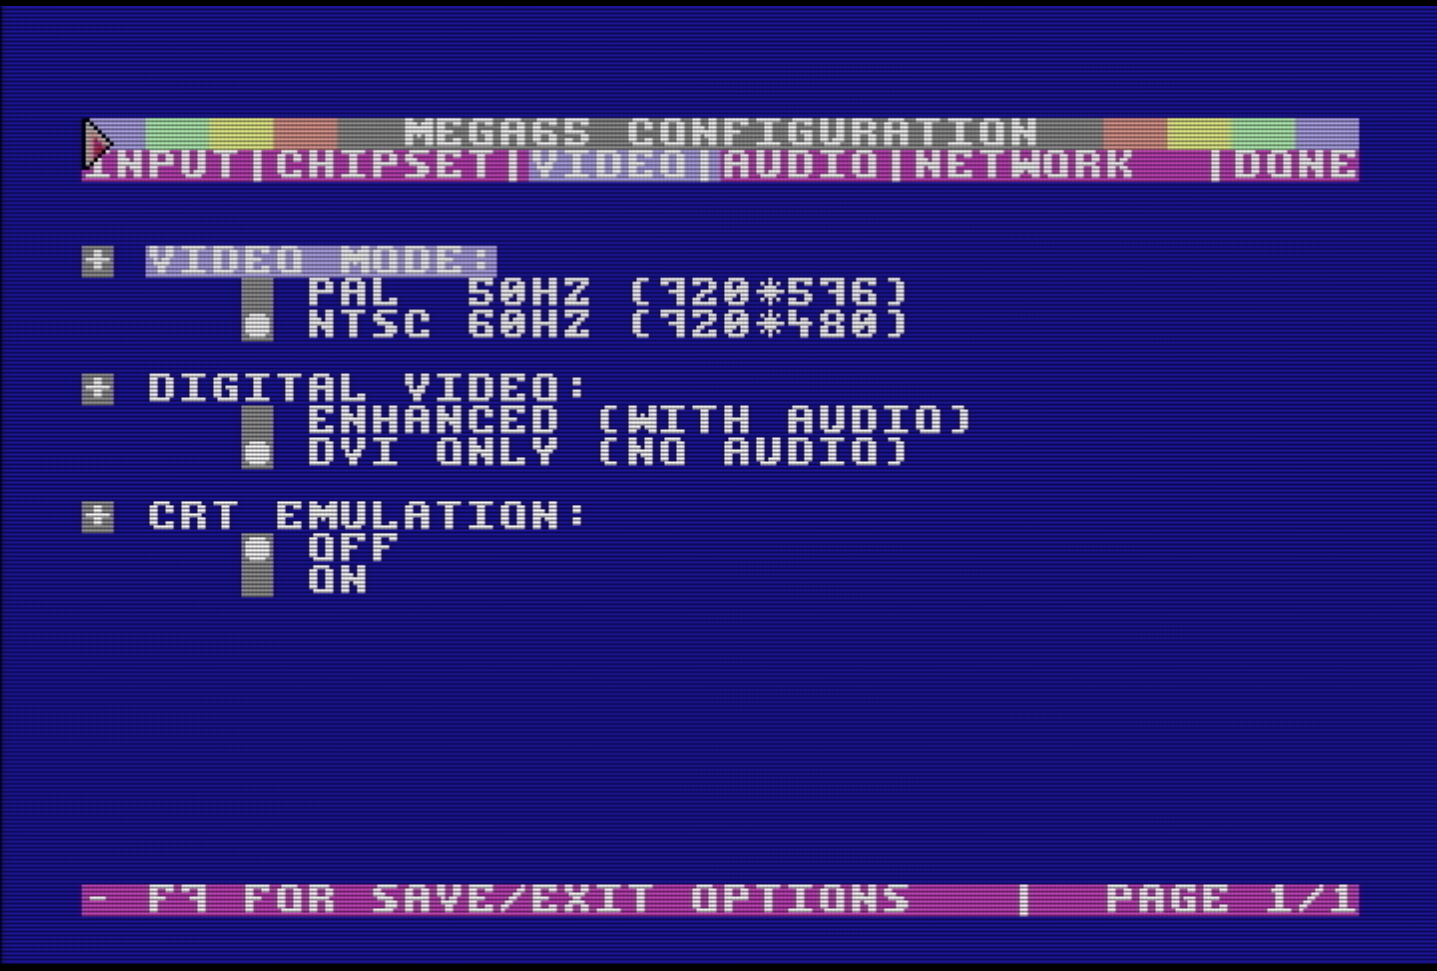
\includegraphics[width=0.7\linewidth]{images/ss-m65config-3.png}
\end{center}

\subsection{Audio}

The ``Audio'' page configures the MEGA65 sound system.

\begin{center}
  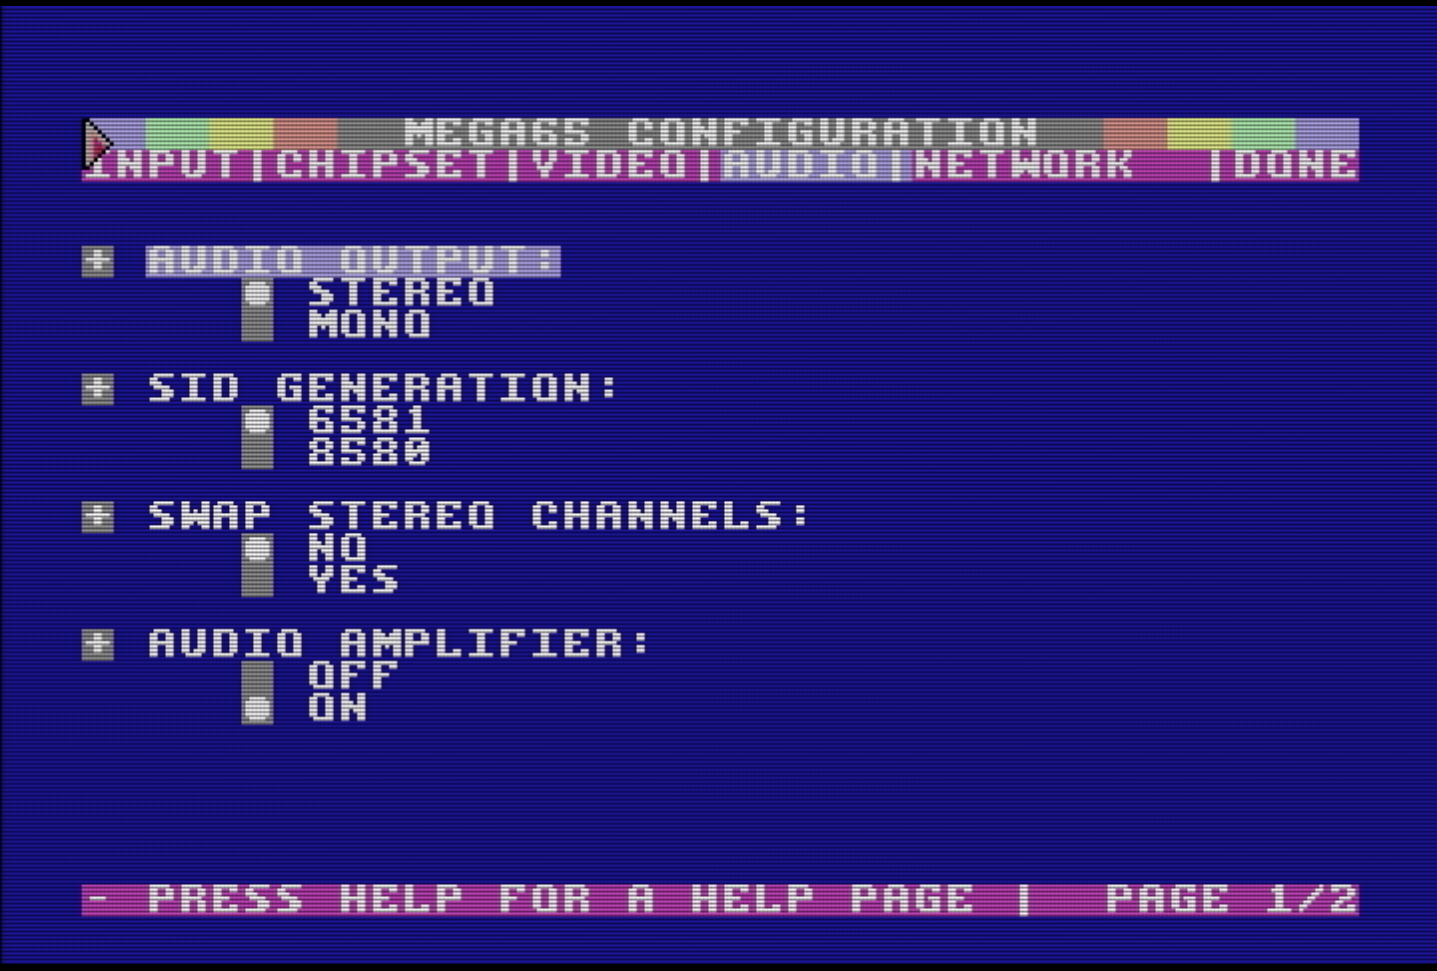
\includegraphics[width=0.7\linewidth]{images/ss-m65config-4.png}
\end{center}

\subsection{Network}

The ``Network'' page gives you the opportunity to adjust the MAC address of the Ethernet port. The MEGA65 does not have a hardware-assigned MAC address. Instead, it uses the value entered here.

If the MAC address is set to all zeros, press the \megakey{R} key to generate a random address. Networking features will not function with an MAC address set to all zeros.

\begin{center}
  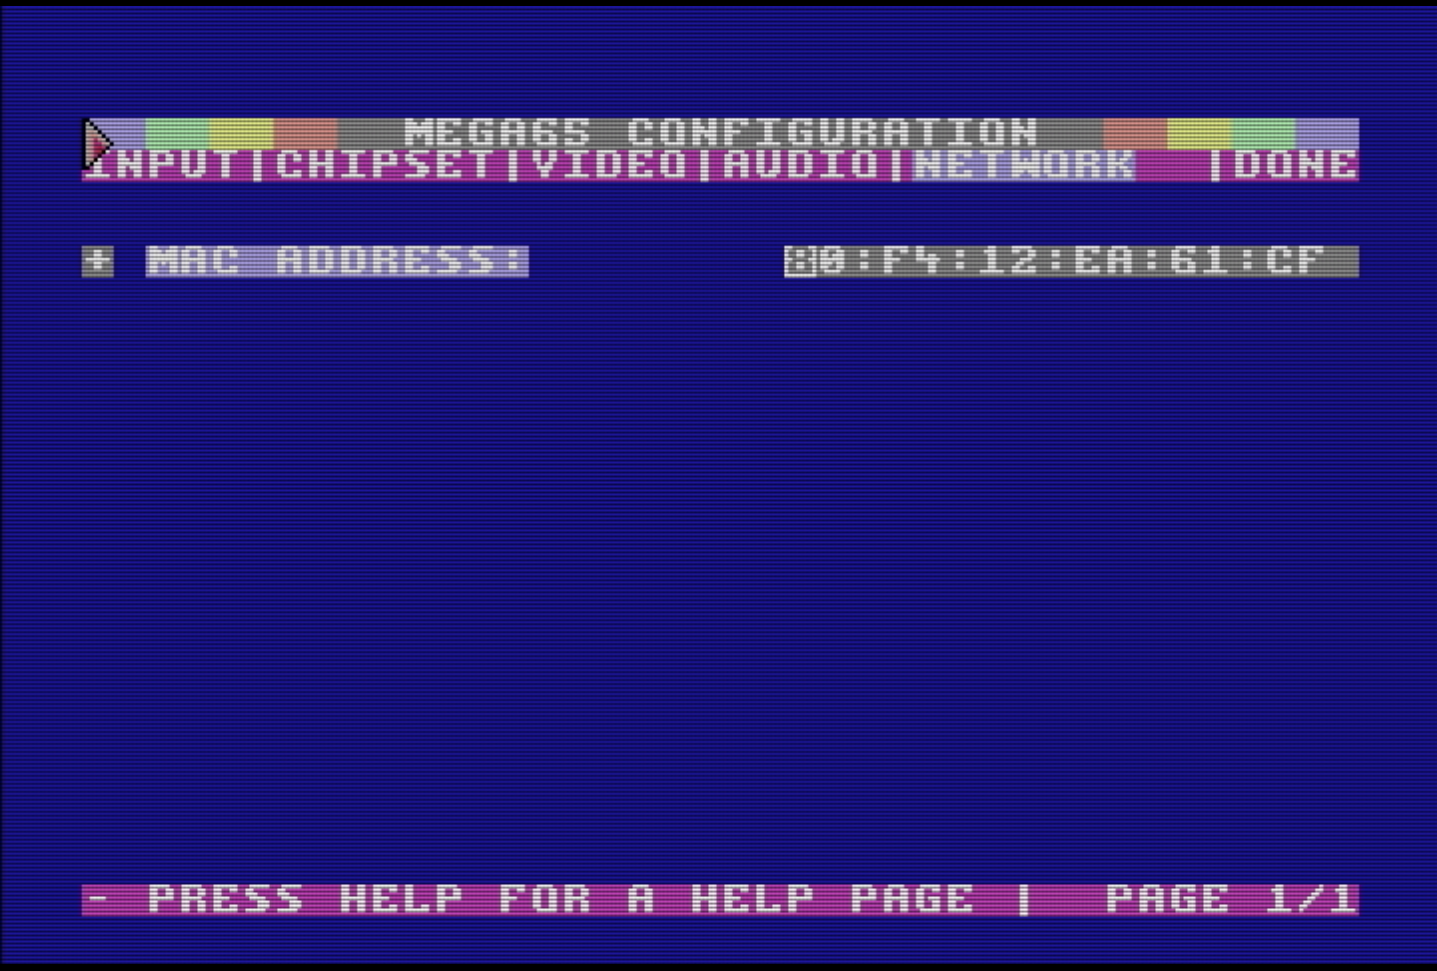
\includegraphics[width=0.7\linewidth]{images/ss-m65config-5.png}
\end{center}

\subsection{Done}

The ``Done'' page lets you exit the Configuration Utility. If you have made changes that you want to keep, select ``Save as defaults and exit.'' You can also abandon changes, restore the factory default settings, or completely restart to the on-boarding screen.

\begin{center}
  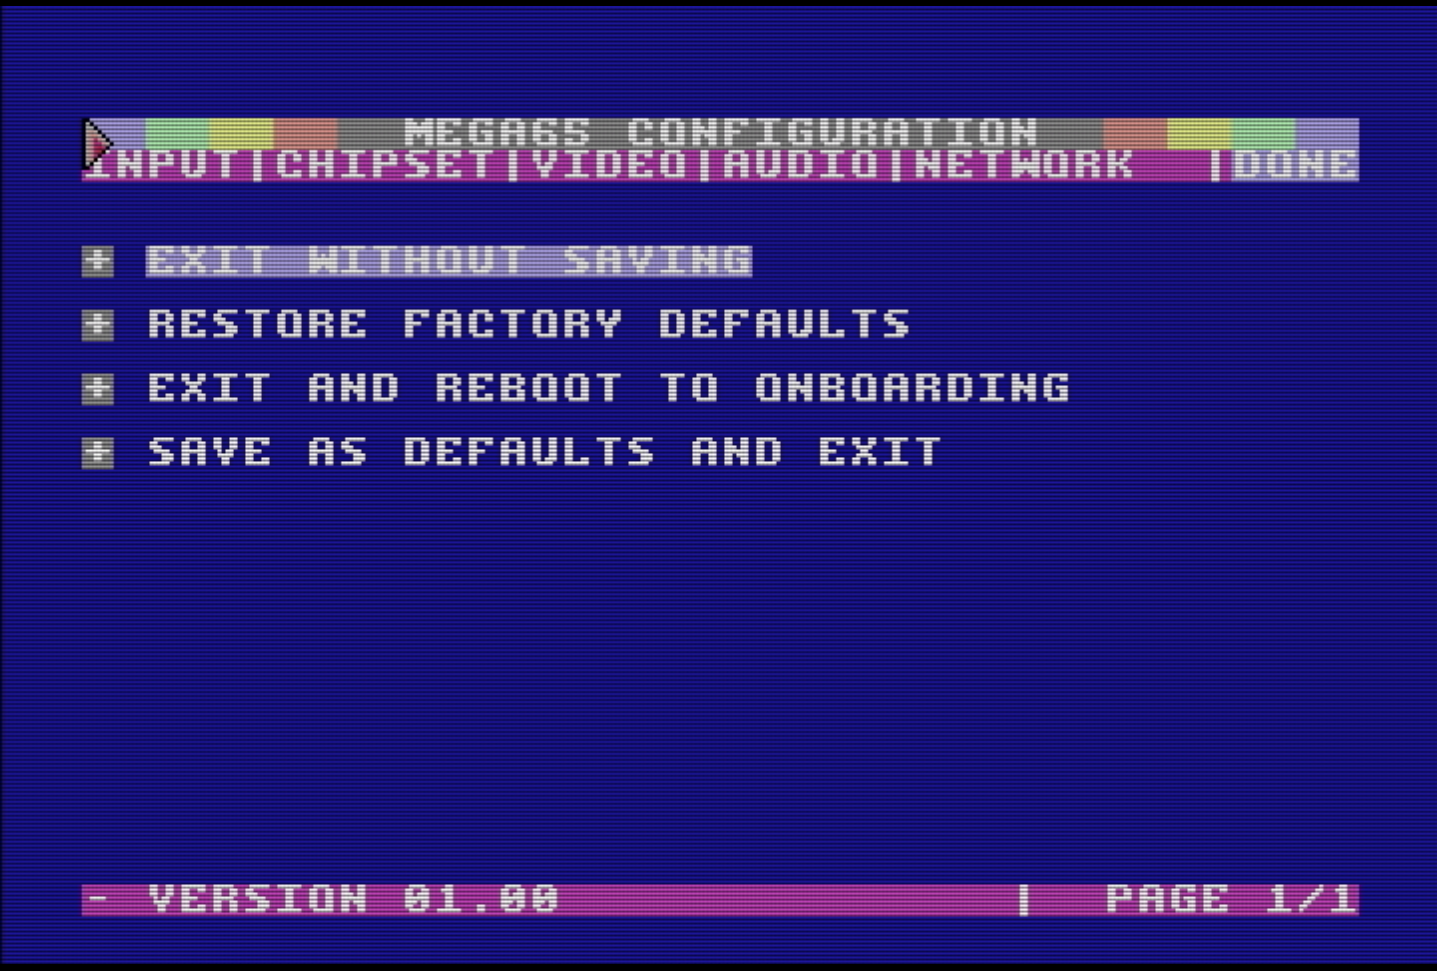
\includegraphics[width=0.7\linewidth]{images/ss-m65config-save.png}
\end{center}


\section{Introducing SD Cards}
\label{sec:introducing-sd-cards}

Your MEGA65 is equipped with two SD card slots: a full-size SD card slot inside the case, and a microSD card slot accessible from the rear of the computer. The MEGA65 uses the SD card for storing configruation settings, loading the operating system, updating the firmware, and storing your software and data as virtual disk images.

The MEGA65 includes a full-size SD card installed in the internal SD card slot, pre-populated with the operating system files and bundled software.\footnote{You can recreate the original SD card's contents using files that you can download from the Internet. Nevertheless, you may wish to make a backup of the SD card contents onto your PC.} You can connect your MEGA65 and start using it immediately without setting up a new SD card. You may wish to leave this SD card in place and pretend that it isn't there, as if your MEGA65 is a computer from the 1990s, with a magical abilility to store data.

The MEGA65 only uses one of the two SD card slots at one time. If there is a microSD card in the rear slot, the internal SD card is ignored. Which slot you use depends on how you expect to use the computer. As you get more familiar with your MEGA65, you may want to move the SD card between the MEGA65 and your PC to copy files and perform system updates. This is more convenient with the external microSD card slot.

Alternatively, you can connect your MEGA65 to your PC or local network with an Ethernet cable, and use a tool to transfer files between the two computers. The file transfer feature accesses files on the SD card, and uses whichever card slot is active.

\section{Preparing a New SD Card}

You can use the microSD memory card slot on the rear of the MEGA65 as persistent storage for the computer's configuration and system files. Having a prepared card in this slot overrides the SD card installed inside the computer. Having a microSD card installed is convenient if you wish to move it between your MEGA65 and your PC.

The following instructions apply to memory cards in either the external microSD card slot or the internal full-size SD card slot.

The MEGA65 supports SD cards of type SDHC, with sizes between 4 gigabytes and 32 gigabytes. Older cards smaller than 4GB and newer SDXC cards larger than 32GB are not expected to work.

An SD card must be prepared by the MEGA65 before use, using the SD Card Utility. The utility creates two partitions: a hidden partition for configuration and freeze state data, and a FAT32-compatible partition for disk images and system files. You can access the FAT32 partition by connecting the SD card to your PC.

An SD card formatted by another computer will {\em not} work with the MEGA65, even if it only erases the FAT32 partition. You {\em must} use the MEGA65 SD Card Utility to format the card.

\subsection{Inserting the SD Card}

Formatting an SD card erases its contents, and this operation cannot be undone. We recommend that you do not erase the internal SD card that came with the computer.

The SD Card Utility will prompt you to select which of the cards currently inserted in the computer to format. As a precaution, you may wish to remove the internal SD card before opening the SD Card Utility. You can reinstall it later, or leave it out of the machine until you need it. This is also a good opportunity to copy the bundled software files off of the internal SD card to your PC, so they can be copied back to the new SD card later.

The utility menu is accessible even if no valid SD card is present. You can bootstrap a new system using just a compatible SD card and the SD Card Utility.

Insert the SD card that you wish to prepare before proceeding.

\subsection{The SD Card Utility}

You access the SD Card Utility from the utility menu. Switch off the MEGA65, hold the \megakey{ALT} key and switch it on again. From the menu, select option \megakey{2} to start the SD Card Utility.

\begin{center}
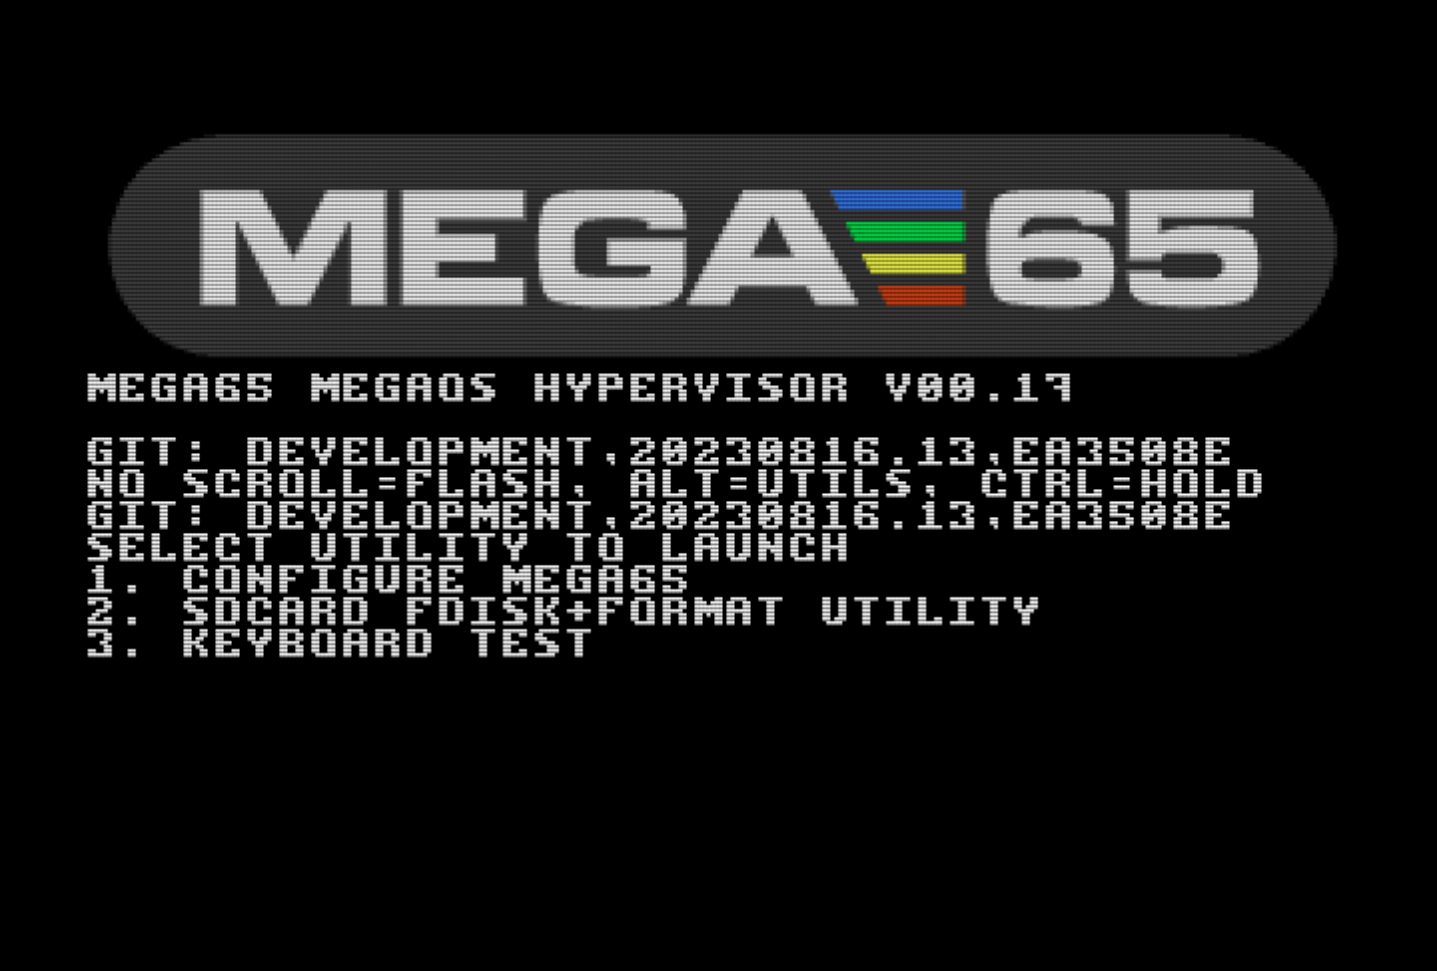
\includegraphics[width=0.7\textwidth]{images/ss-utilmenu.png}
\end{center}

The SD Card Utility opens and looks for SD cards installed in the slots. If you haven't inserted the SD card that you want to prepare yet, do so now, then press \megakey{R} to re-scan.

\begin{center}
  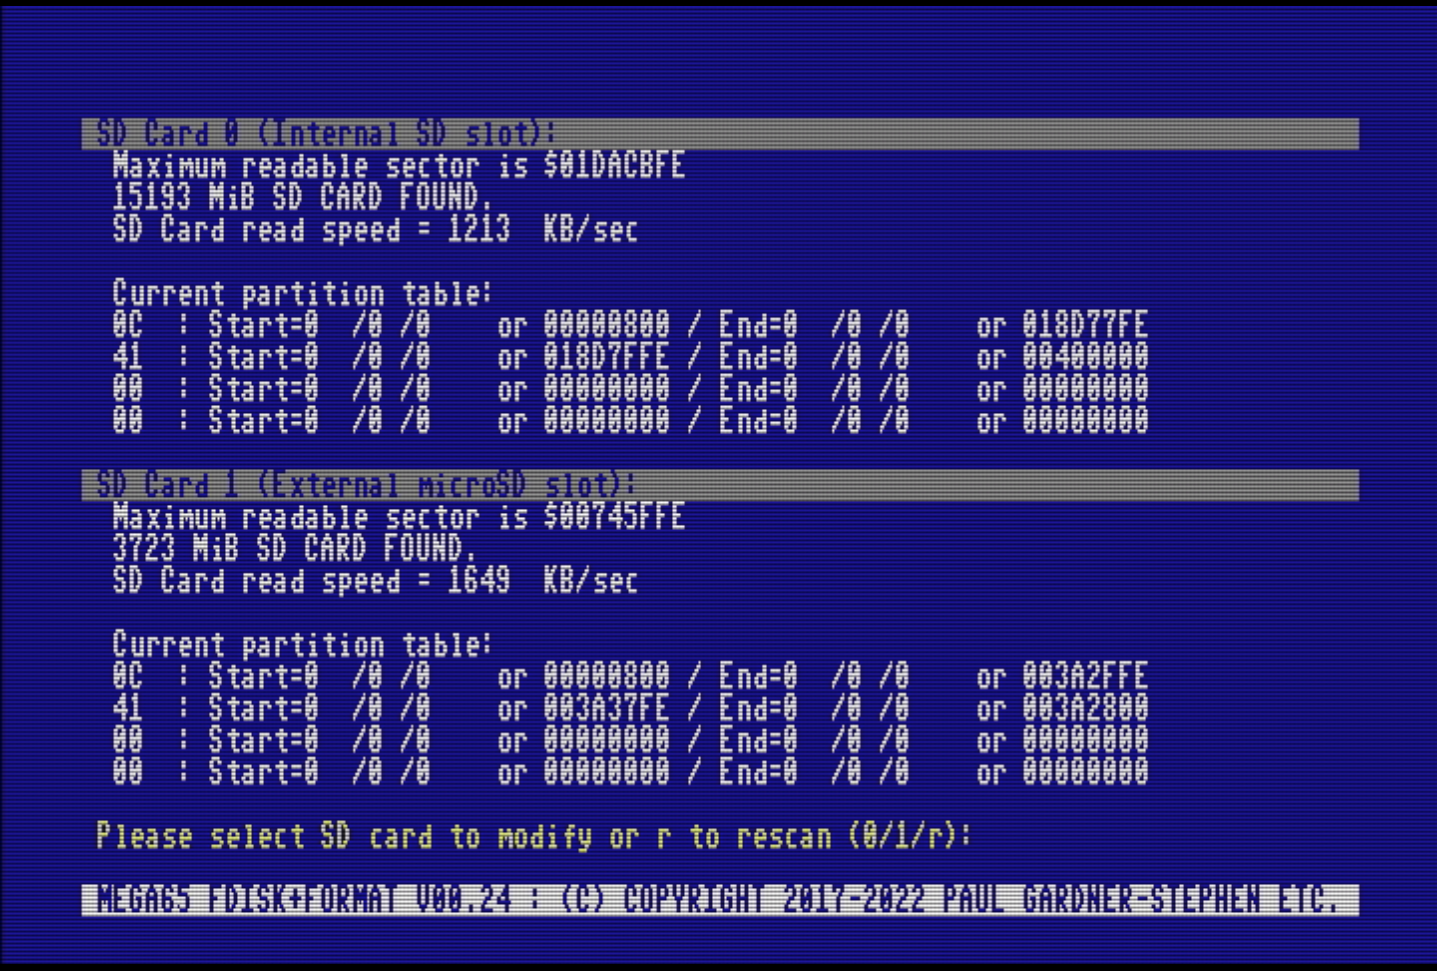
\includegraphics[width=0.7\textwidth]{images/ss-m65fdisk-busselect.png}
\end{center}

Select the card that you want to prepare: \megakey{0} for the internal SD card, \megakey{1} for the external microSD card. If you have two cards installed, {\em be careful to choose the correct card slot.}

The SD Card Utility prompts for confirmation to erase the SD card. As one last precaution, you must type the phrase {\tt DELETE EVERYTHING} in all capital letters to proceed. (If you wish to abort this process, it is safe to switch off the MEGA65 at this time.)

\begin{center}
  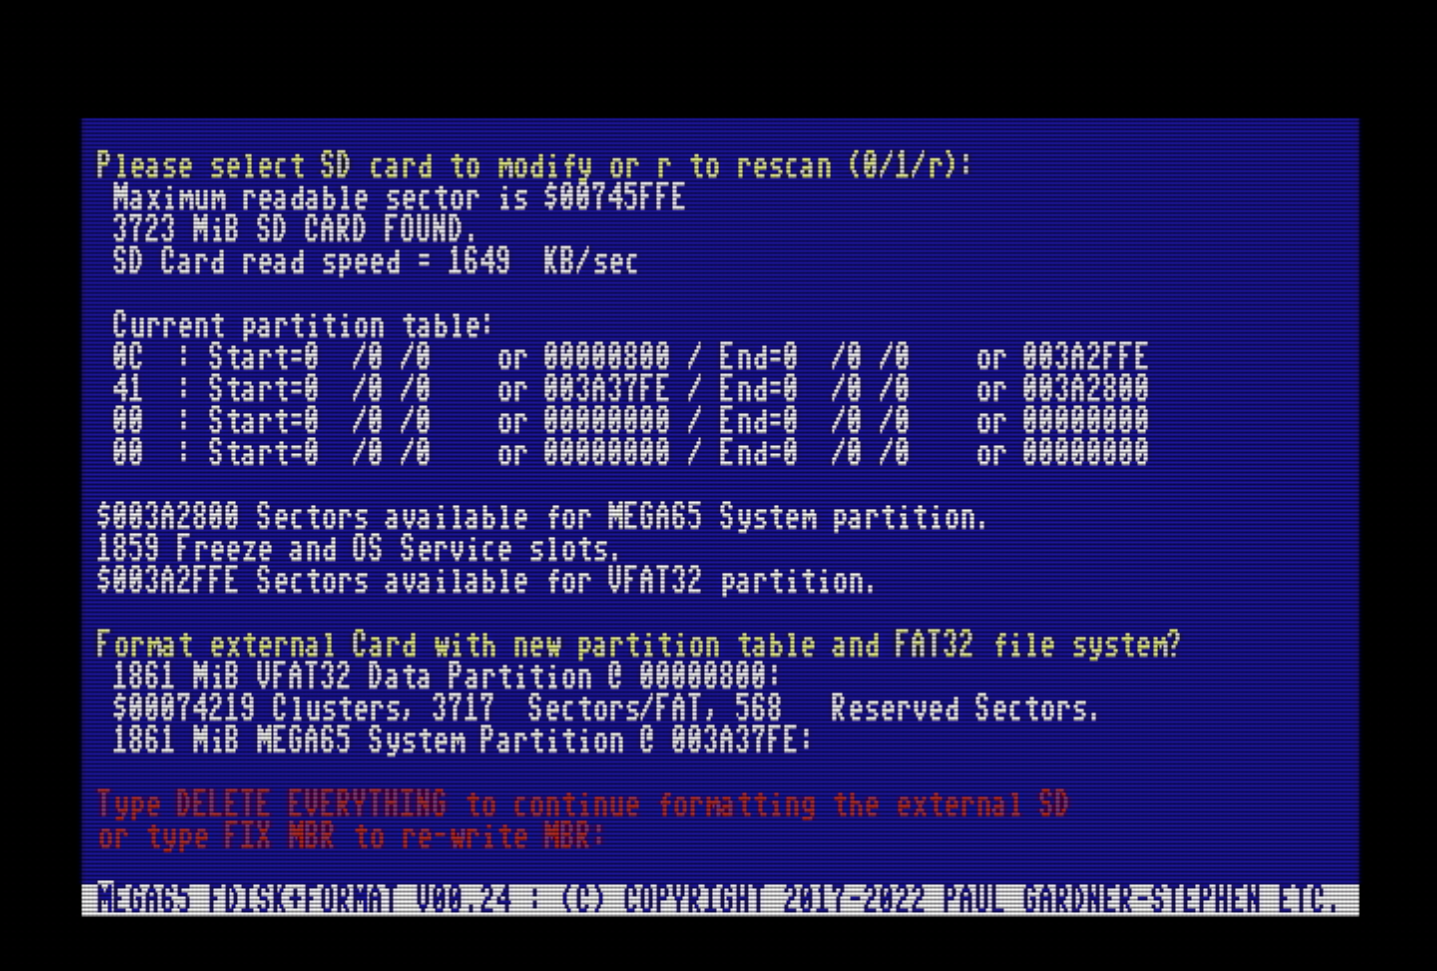
\includegraphics[width=0.7\textwidth]{images/ss-m65fdisk-typesomething.png}
\end{center}

The utility erases the SD card and sets up the partitions. When it is finished, it prompts to install the system files embedded in the MEGA65 chipset core. If you have installed an updated MEGA65 core in slot 1, select it, otherwise select the factory-installed MEGA65 core in slot 0. (If you just received your MEGA65, slot 0 is the only option.)

\begin{center}
  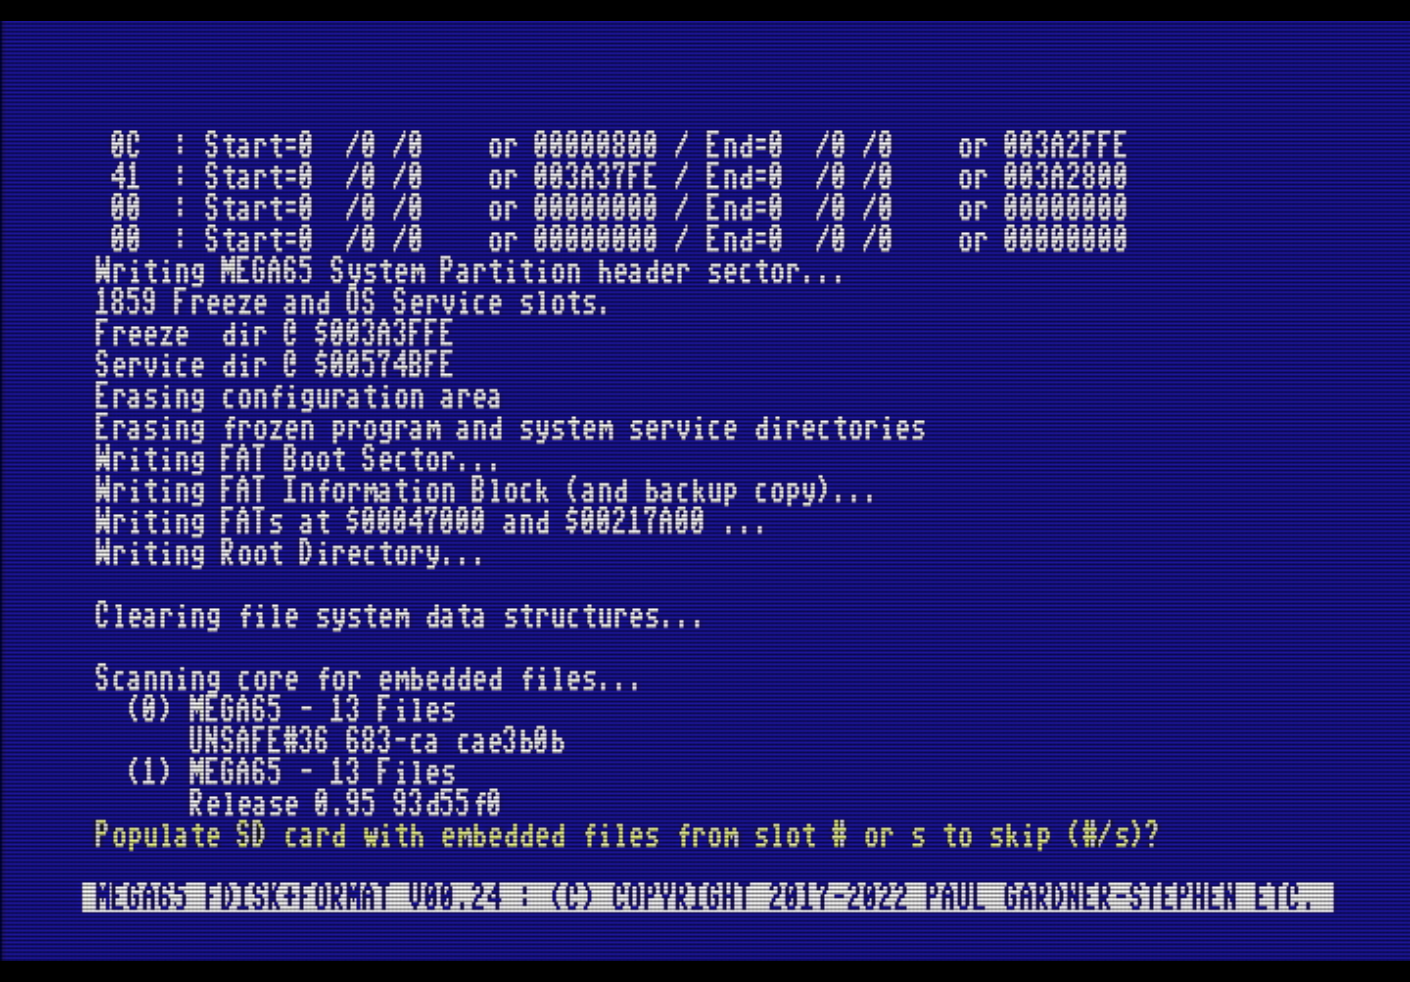
\includegraphics[width=0.7\textwidth]{images/ss-m65fdisk-populate.png}
\end{center}

When prompted, reboot the machine.\footnote{If you select a core that does not have {\tt MEGA65.ROM} as one of the embedded files, the utility will prompt you to move the SD card to your PC to copy this file onto it. This only happens when using a MEGA65 core from somewhere other than an official MEGA65 release package. For more information about cores and obtaining {\tt MEGA65.ROM}, see chapter \vref{cha:cores}.}

\subsection{Obtaining the Bundled Software}

The system files copied to the freshly formatted SD card do not include the bundled software that was included with the original SD card in the internal card slot. You can use your PC to copy these files off of the original SD card, then copy them back onto the new SD card.

The MEGA65 Filehost website hosts all manner of files you can download for your MEGA65. This includes the latest versions of the platform components, alternate cores, and hundreds of games, demos, and applications produced by the MEGA65 community. This also includes the bundled software from the original SD card included with the computer.

If you no longer have the bundled software files, you can obtain them from the MEGA65 Filehost website. Visit the following URL, then search for ``MEGA65 Release SD Card - Intro Disk Extras.''

\url{https://files.mega65.org}

\chapter{Upgrading the MEGA65}
\label{cha:cores}

\section{How a MEGA65 Can Be Upgraded}

The MEGA65 platform consists of three major components:

\begin{enumerate}
  \item The {\bf MEGA65 core}, a description of the chipset to run on the FPGA
  \item The {\bf ROM}, code that defines the Commodore-style operating system (kernel) and BASIC
  \item {\bf System software} for features such as the Freezer menu
\end{enumerate}

You can upgrade these components as new releases are published. You can also replace one or more of these components individually. In the case of the core and ROM, you can even have multiple versions installed simultaneously and switch between them. For example, instead of the latest MEGA65 ROM, you can switch to the original Commodore 65 prototype ROM. Or, you could switch to another core that causes your MEGA65 hardware to behave like a different computer entirely, such as a Commodore 64 or a ZX Spectrum.

The ROM and system software are files that reside on the SD card, and upgrading them is as simple as replacing the files. To upgrade the core, you use a process to install a core file into the MEGA65's core flash memory. This chapter describes this process.

\subsection{What is a Core?}

The MEGA65 hardware architecture is based on a versatile chip called a ``Field Programmable Gate Array,'' or FPGA. This is a special kind of computer chip that can be programmed to impersonate other chips. They do this by configuring a giant array of logic gates to reproduce circuits. FPGAs are not an emulation, but an electronic re-creation of other chips. FPGA code is sometimes referred to as {\em firmware,} a term you may recognize from modern computers and other devices.

Your MEGA65 was programmed at the factory to re-create a chipset designed by the MEGA65 team, based on the original Commodore 65. You can re-program the MEGA65 FPGA to upgrade to new versions of the MEGA65 chipset, or to replace the chipset with that of an entirely different computer!

Each possible chipset is known as a {\em core}. The MEGA65 can store up to eight cores, and you can switch between these cores by accessing a menu when you switch on the computer. You can also use this menu to load a new core from a file on the SD card, a process known as {\em flashing}.

Members of the MEGA65 community have made several useful and fun alternate cores for the FPGA hardware. \href{https://github.com/MJoergen/C64MEGA65}{{\em C64 for MEGA65}} by MJoergen and sy2002 re-creates the original Commodore 64 computer with a high degree of accuracy, perfect for running Commodore 64 games, demos, and applications. Other cores re-create the ZX Spectrum, the Game Boy, and even the original Galaga arcade machine hardware. The MEGA65 team believes that the FPGA is powerful enough to re-create nearly all 8-bit home computers, and likely some 16-bit computers and consoles such as the Commodore Amiga. The MEGA65 hardware design, board layout, FPGA core, and other information are all available for free under various open-source licenses, so anyone is free to
create other cores for the MEGA65 hardware.

\section{Determining the Versions of Things}
\label{sec:versions}

All components of the MEGA65 platform have a version identifier. The MEGA65 can display the version identifiers for all of its components using the ``MEGA65 Information'' utility.

To open the ``MEGA65 Information'' utility:

\begin{enumerate}
  \item Switch on the MEGA65, and allow it to boot to BASIC.
  \item Open the Freezer: press and hold \widekey{RESTORE} for one second then release it.
  \item Press \specialkey{HELP}. The ``MEGA65 Information'' utility will open.
\end{enumerate}

\begin{center}
  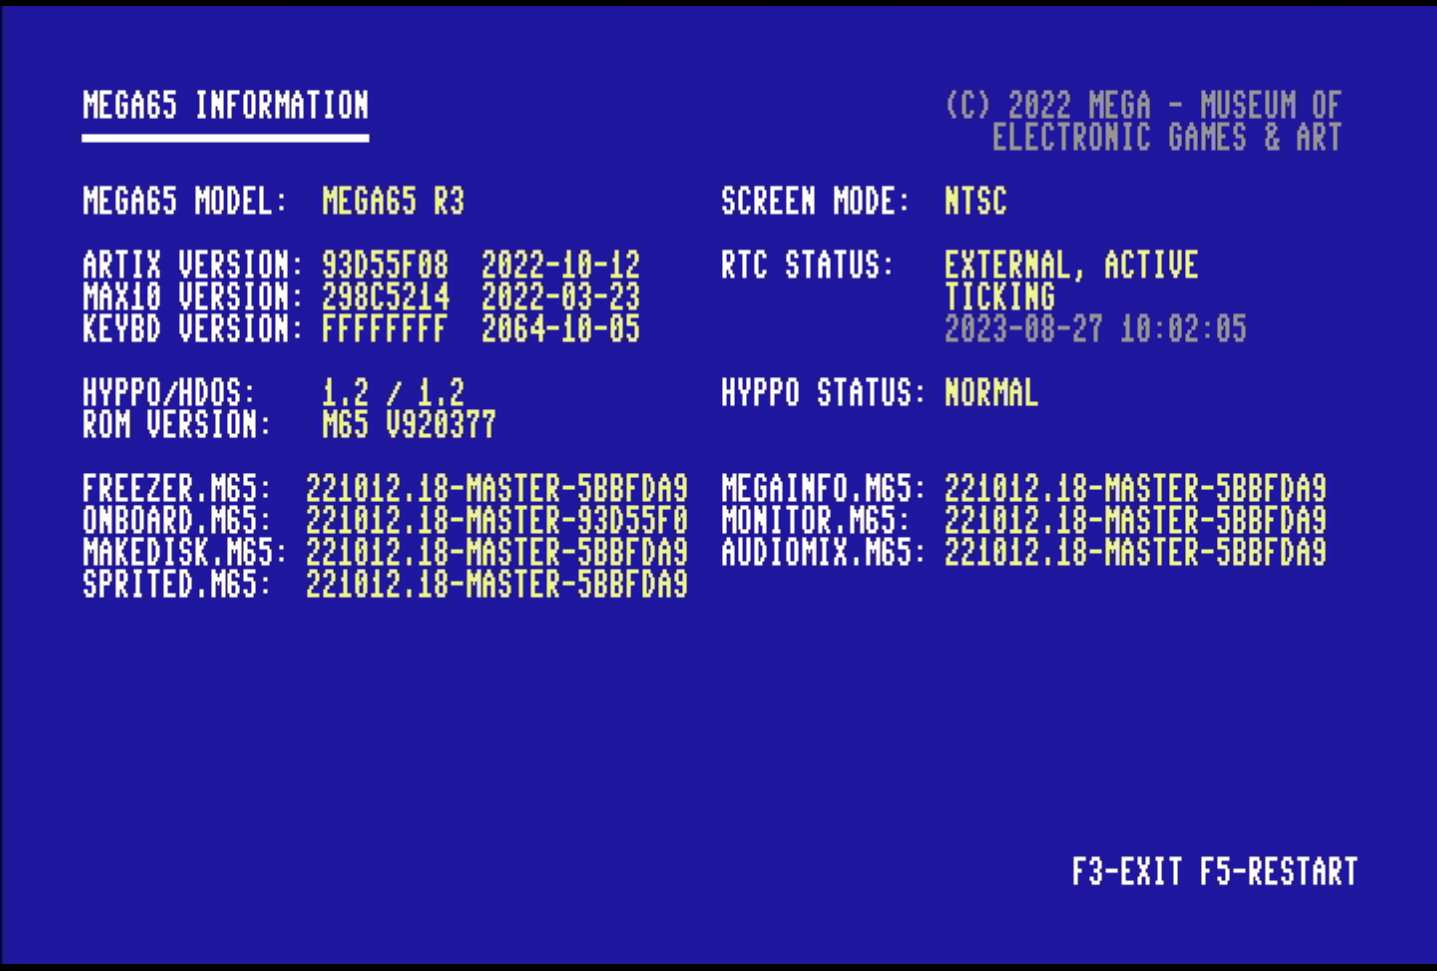
\includegraphics[width=0.7\linewidth]{images/megainfo.png}
\end{center}

Take note of these version identifiers:

\begin{center}
\setlength{\tabcolsep}{1mm}
\begin{tabularx}{\textwidth}{|X|p{7cm}|}
  \hline
  {\bf Label and Example} & {\bf Description} \\
  \hline
  MEGA65 Model\newline {\tt MEGA65 R5} & The revision of the hardware. You need to know this when downloading new core files. \\
  \hline
  Artix Version\newline {\tt 93D55F08 2022-10-12} & The currently running MEGA65 core. This is a string of eight letters and numbers, and also a build date. \\
  \hline
  ROM Version\newline {\tt M65 V920377} & The currently running ROM. For MEGA65 ROMs, this is a sequential number, with larger numbers representing newer releases. \\
  \hline
  System files (.M65)\newline {\tt 221012.18-MASTER-5BBFDA9} & Each of the system software files has its own version identifier. Typically, you do not need to know these: you will upgrade these along with each core. The identifier is similar to the core version, but does not always match the currently running core. \\
  \hline
\end{tabularx}
\end{center}

Press \specialkey{F3} to exit to the Freezer, then \specialkey{F3} again to exit to BASIC.

Each core has a separate version for each hardware revision. As of the year 2023, the production models of the MEGA65 have used two different main board revisions, known as ``R3'' (more specifically ``R3A'') and ``R5.''\footnote{The MEGA65 ``DevKit'' model sold in the year 2020 is revision ``R3.'' It is also possible to run the MEGA65 core on certain FPGA development boards, with a separate version of the core file for each.}

The MEGA65 core is available for all hardware revisions. If you are installing an alternate core and it is not available for your hardware revision, contact the author of the core.

\section{Obtaining the Latest Files}

You can download the latest MEGA65 core, ROM, and system software from the MEGA65 Filehost website. Due to distribution restrictions for the Commodore 65 ROM code, some files require a Filehost account registered to a MEGA65 owner to access. All owners of the MEGA65 have a license to all versions of this ROM code.\footnote{There is a procedure for non-owners to get the latest MEGA65 ROM, such as to use with the \href{https://github.lgb.hu/xemu/}{Xemu MEGA65 emulator}. This involves downloading \href{https://www.c64forever.com/}{C64 Forever Free Express Edition} from Cloanto, extracting the original Commodore 65 prototype ROM file, then using a tool to apply a patch that you can download from Filehost. The full process is described in the following article: \url{https://files.mega65.org?ar=145591dd-deb6-4bd0-aa89-8e39cd021470}}

Visit the following URL in your web browser:

\url{https://files.mega65.org}

\begin{center}
  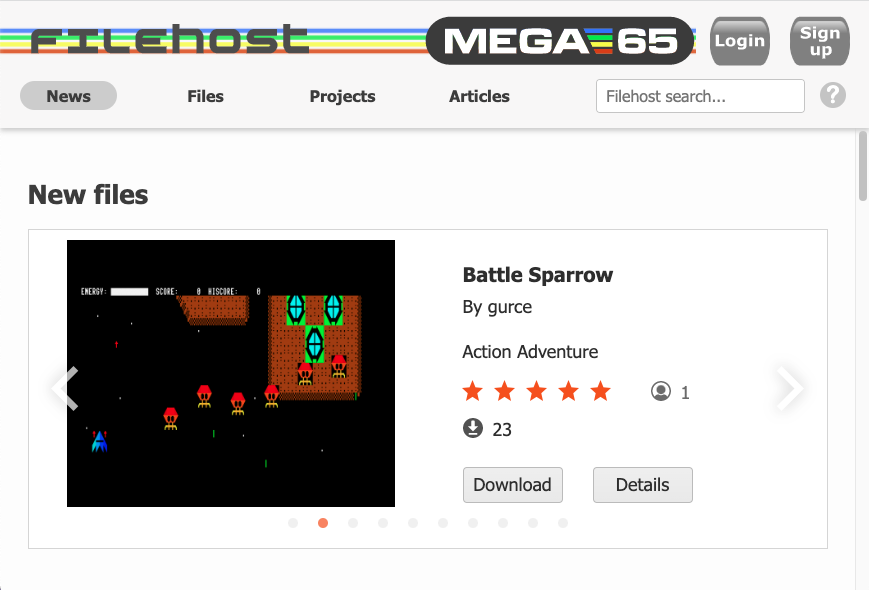
\includegraphics[width=0.7\linewidth]{images/filehost_notsignedin.png}
\end{center}

To register a Filehost account with your owner code:

\begin{enumerate}
  \item Visit \href{https://files.mega65.org}{Filehost}. Click ``Sign Up.'' Follow the prompts to create an account.
  \item Locate your owner code. This is a code printed on a piece of paper that was included with your MEGA65 (possibly inserted into this manual). It looks something like this: {\tt 123-ABC-456}
  \item Click the user icon in the upper-right corner of the Filehost screen. In the pop-up menu, select ``Redeem Code.'' Enter your owner code as prompted.
\end{enumerate}

\begin{center}
  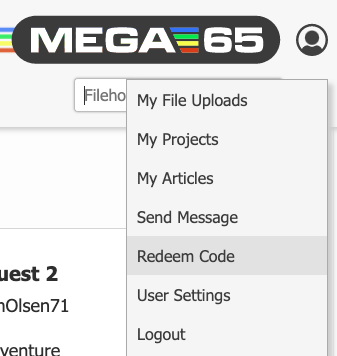
\includegraphics[width=0.4\linewidth]{images/filehost_redeemmenu.png}
\end{center}

To download the latest release package:

\begin{enumerate}
  \item Click the ``Files'' tab of the Filehost website.
  \item In the search box on the left-hand side, enter ``release''. The list will update to show only files with that word in the title.
  \item Locate the entry named, ``MEGA65 Core Release Package (mega65r3) incl. ROM,'' where ``mega65r3'' matches your hardware revision.
  \item Click the entry. Confirm that this release package is for your hardware revision, then click ``Download'' to download the file.
\end{enumerate}

If you don't see an entry that says ``incl. ROM,'' check that you are signed in and that you have redeemed a valid owner code. Note that there is an entry for the Release Package that does not include the ROM that is visible to everyone. To ensure you are using a compatible set of files, get the package that says ``incl. ROM.''

\begin{center}
  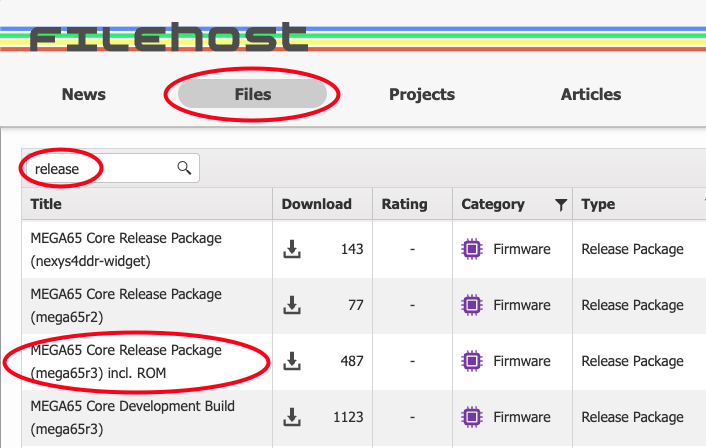
\includegraphics[width=0.7\linewidth]{images/filehost_release.png}
\end{center}

Expand the downloaded archive. You should see a file whose name ends in {\tt .cor}, and a folder of {\tt sdcard-files} that includes one named {\tt MEGA65.ROM}.

\section{The Core Selection Menu}

The MEGA65 decides which core to load into the FPGA when it starts up. You can interrupt this process to select which core to load.\footnote{Technically, the MEGA65 starts the core in slot 0 to power the core selection menu. After you have made a selection or it chooses a default, it loads the selected core into the FPGA and continues the boot process.}

To open the core selection menu, switch off the computer, then hold the \specialkey{NO\\SCROLL} key and switch on the computer. The core selection menu appears, with the eight core slots numbered 0 through 7.

\begin{center}
  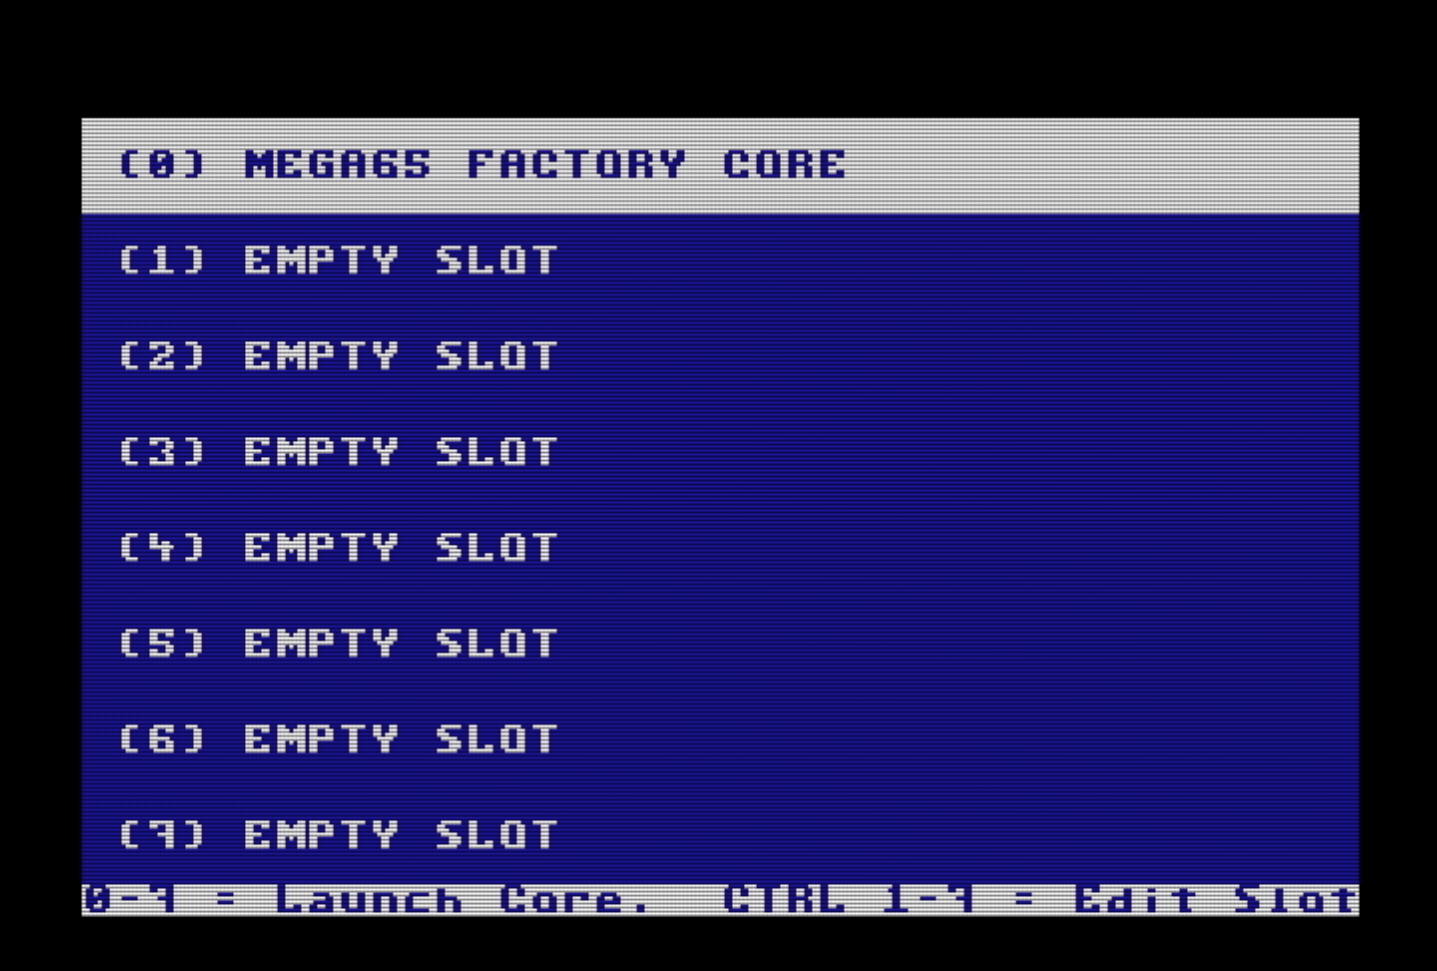
\includegraphics[width=0.7\linewidth]{images/ss-flashmenu.png}
\end{center}

You can select a core to boot using the cursor keys and \specialkey{RETURN}, or you can simply press the number key that corresponds to the slot. The boot process continues with the new core. The MEGA65 will keep running the new core until you physically power it off. (Pressing the reset button will not reset which core is being run.)

When you switch on the computer without opening the core selection menu, the MEGA65 looks for a core in slot 1. If there is a valid core in that slot, it uses it. Otherwise it tries slot 0.\footnote{You can change the default core slot from 1 to 2 by moving DIP switch \#4 to the ``on'' position. DIP switches are located inside the case, on the main board.}

Your computer comes with the MEGA65 core in slot 0 installed at the factory. It is recommended that you do not upgrade the factory-installed core under most circumstances. Instead, install new versions of the MEGA65 core in slot 1.

\section{Upgrading the MEGA65 Core, ROM, and System Files}

You can upgrade a core, or install a new core from the core selection menu. This process reads the {\tt .cor} file from the SD card.

To upgrade the MEGA65 core, ROM, and system files:

\begin{enumerate}
  \item Remove the SD card (or microSD card) from the MEGA65, and connect it to your PC using an SD card reader.
  \item Copy the {\tt .cor} file from the archive you downloaded to the SD card.
  \item On your PC, open the {\tt sdcard-files} folder, then copy those files to the SD card, replacing the existing files. Put them in the root of the SD card's file system, not a sub-folder.
  \item Eject the SD card from your PC's operating system, then move it back to the MEGA65.
  \item Open the core selection menu: Switch off the MEGA65, then hold \specialkey{NO\\SCROLL} while switching it back on.
  \item Hold \specialkey{CTRL} then press the number of the slot you want to upgrade. Follow the prompts. This process asks for a key press several times, and takes several minutes.
\end{enumerate}

When you start the update process, it prompts you to select the {\tt .cor} file on a screen that looks similar to this:

\begin{center}
  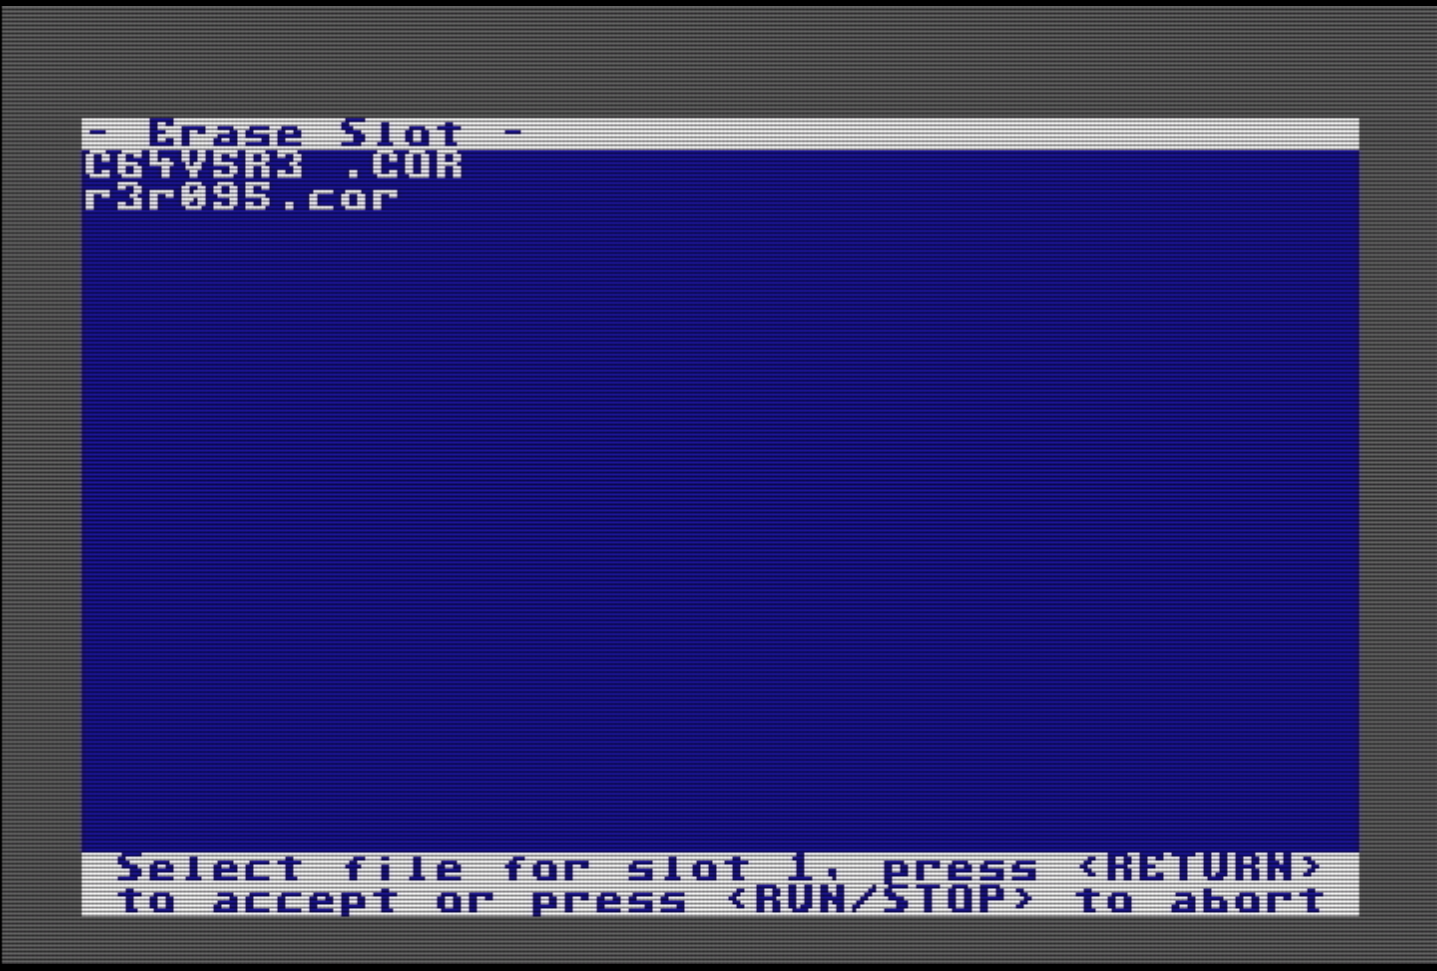
\includegraphics[width=0.7\linewidth]{images/ss-flashmenu-selectcore.png}
\end{center}

The process begins by checking that the core file matches your hardware revision. Press any key to continue.

\begin{center}
  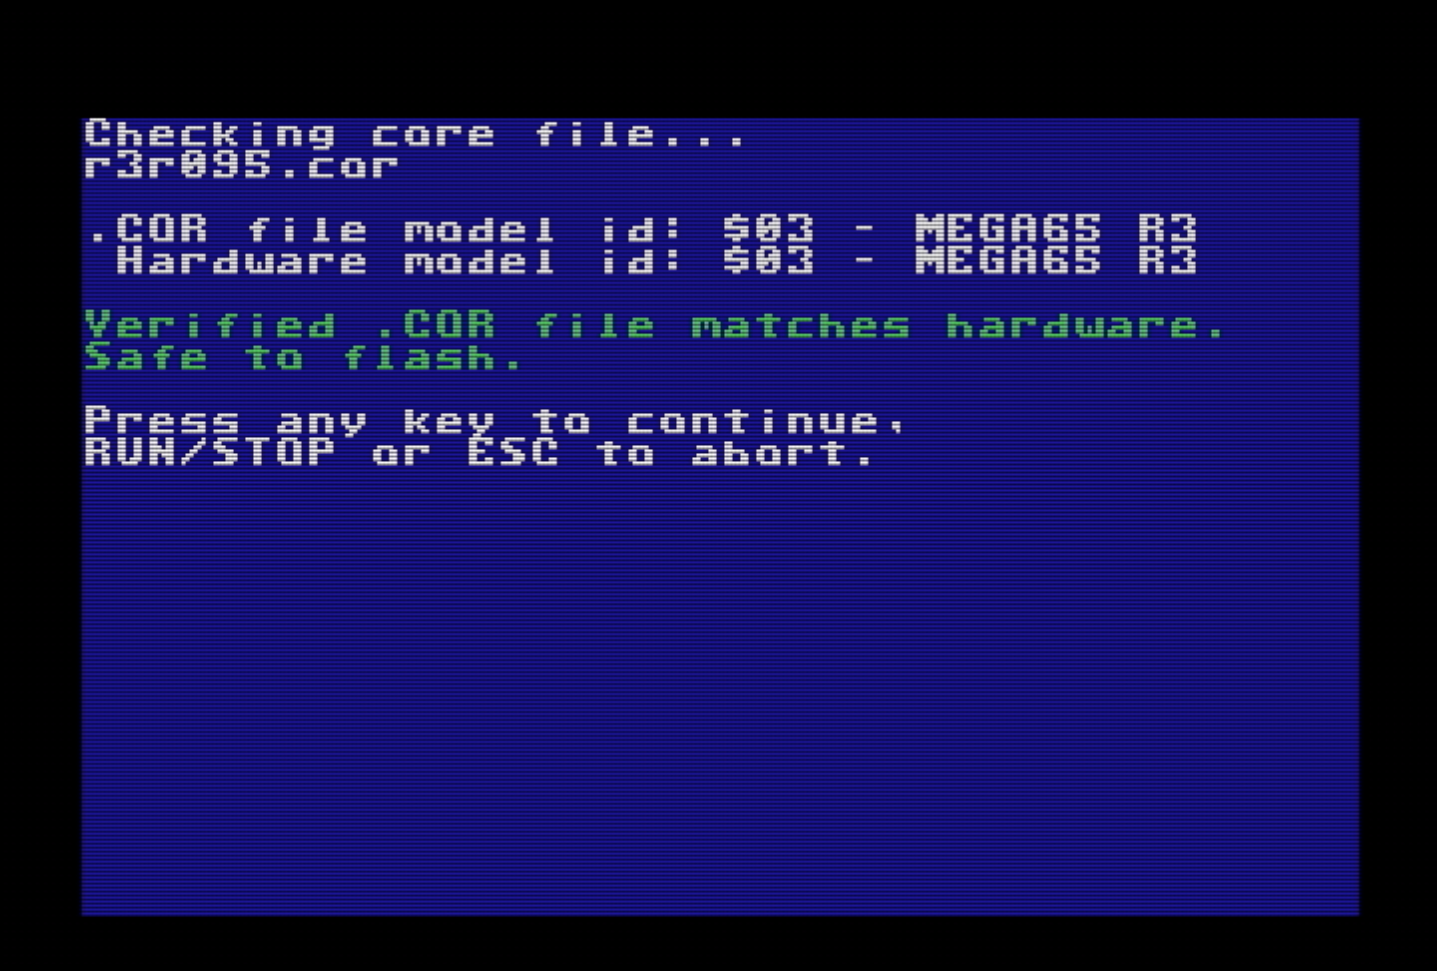
\includegraphics[width=0.7\linewidth]{images/ss-flashmenu-1-checking.png}
\end{center}

It then copies the file from the SD card to RAM, performing another check that the core file is complete.

\begin{center}
  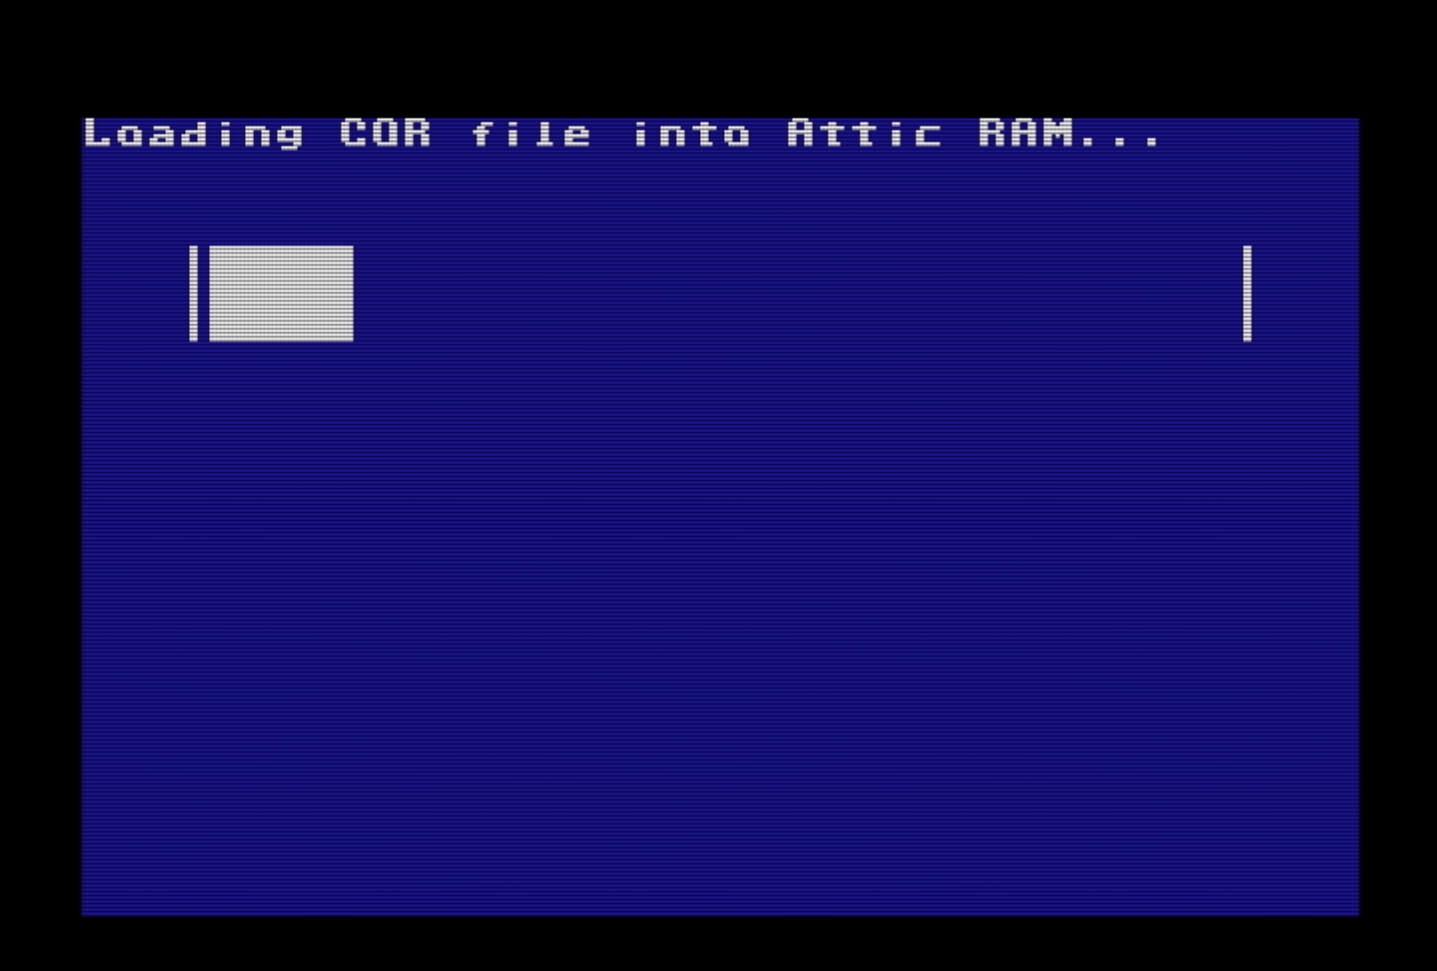
\includegraphics[width=0.7\linewidth]{images/ss-flashmenu-2-loading.png}
\end{center}

It presents the result of this check before proceeding. If the check is valid, you will see a message similar to the following. Press any key to continue.

\begin{center}
  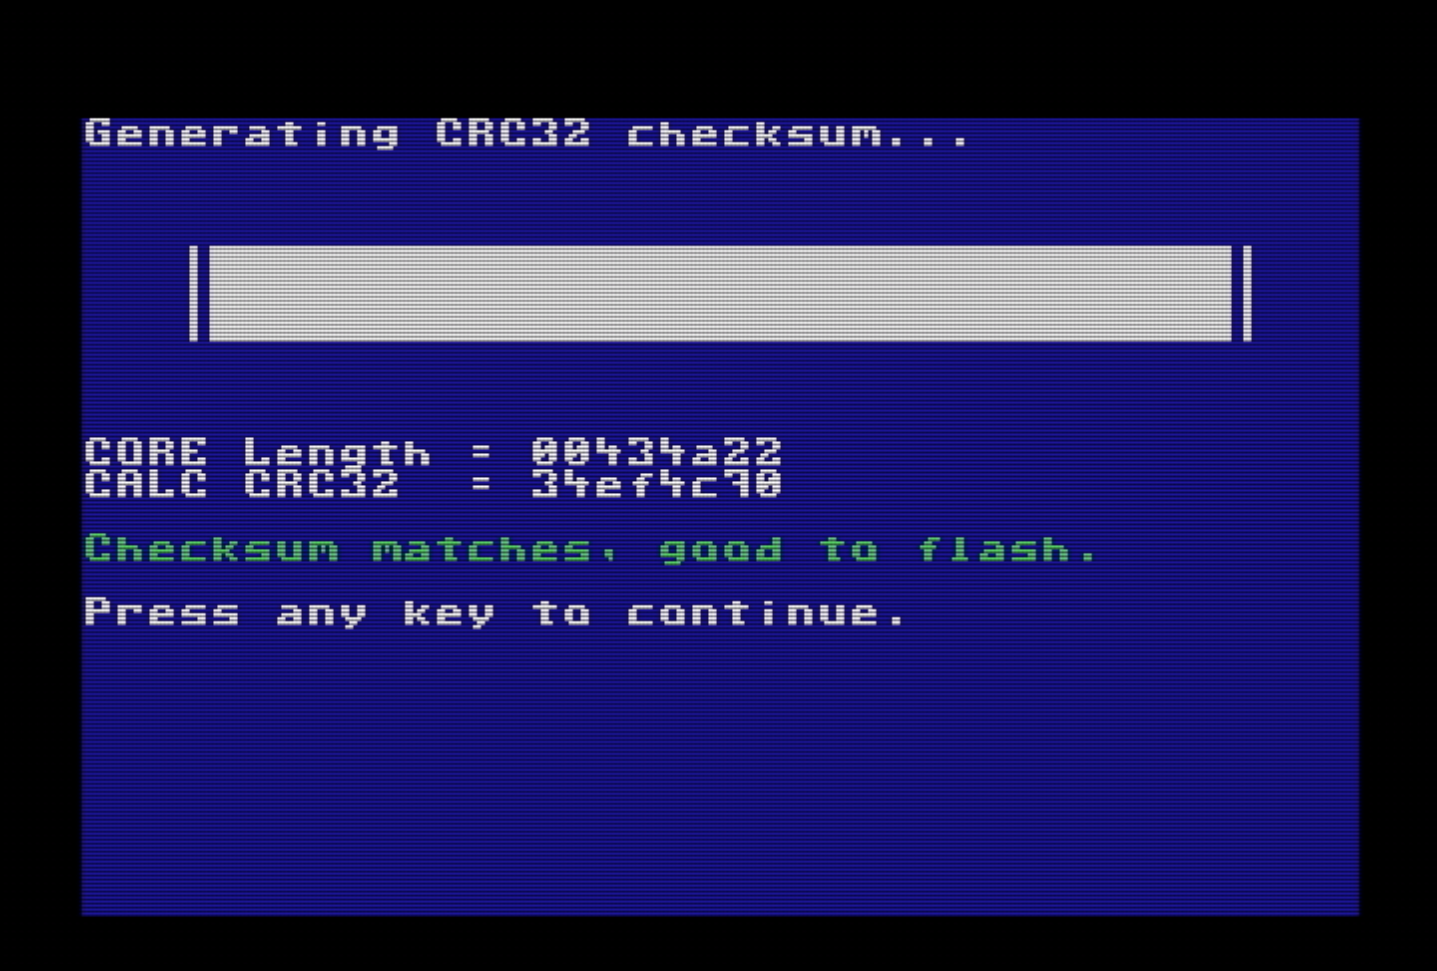
\includegraphics[width=0.7\linewidth]{images/ss-flashmenu-3-checksum-ok.png}
\end{center}

If the check is invalid, you will see a message similar to the following. If you were not expecting this message, abort the process and confirm that you are using the correct file.\footnote{There are rare cases where a core may be valid but not have a correct checksum, such as if you are installing older versions of the core.}

\begin{center}
  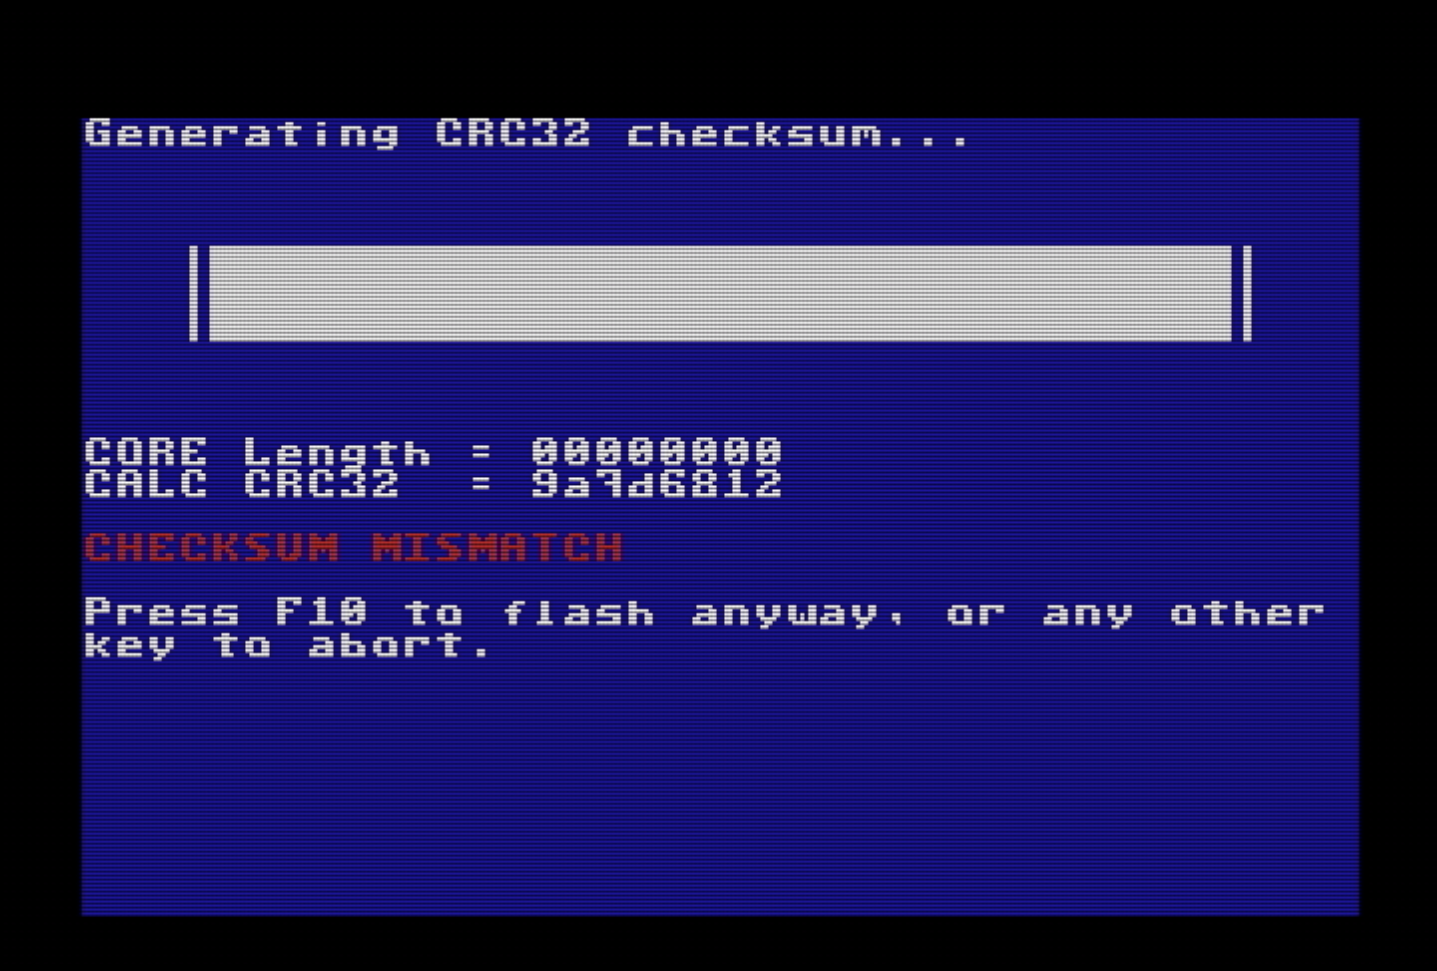
\includegraphics[width=0.7\linewidth]{images/ss-flashmenu-3-checksum-mismatch.png}
\end{center}

Once you tell it to proceed, the MEGA65 begins programming the core data into flash memory. The border twinkles in coloured patterns during this process.

\underline{Note}: Do {\em not} switch off your computer or disconnect power until after this step is complete.

\begin{center}
  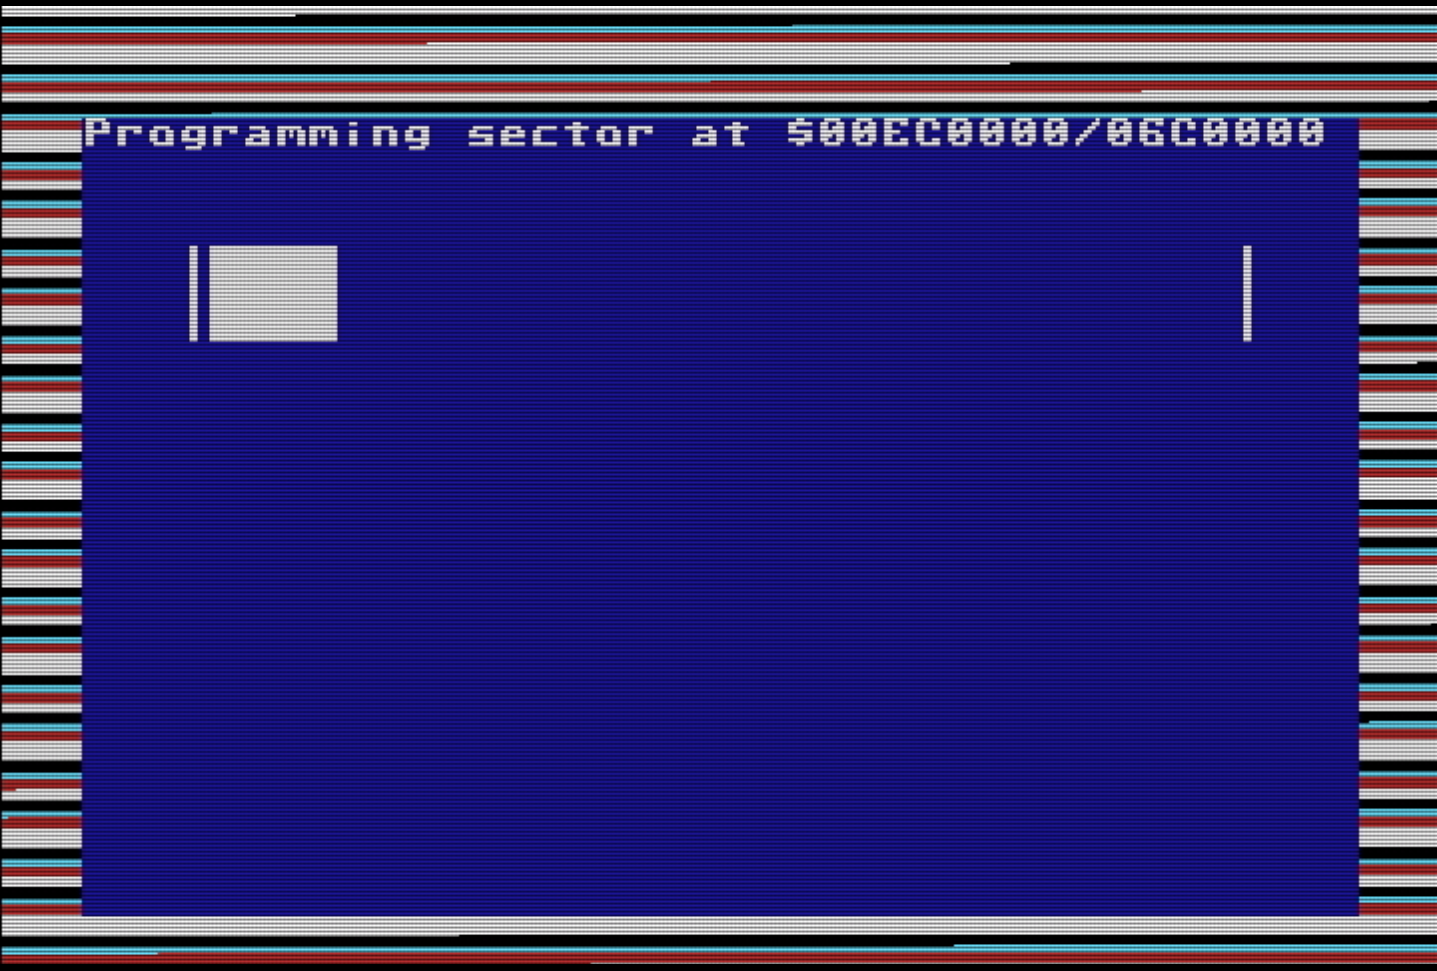
\includegraphics[width=0.7\linewidth]{images/ss-flashmenu-4-programming.png}
\end{center}

When the process is complete, you will see a screen similar to the following.

\begin{center}
  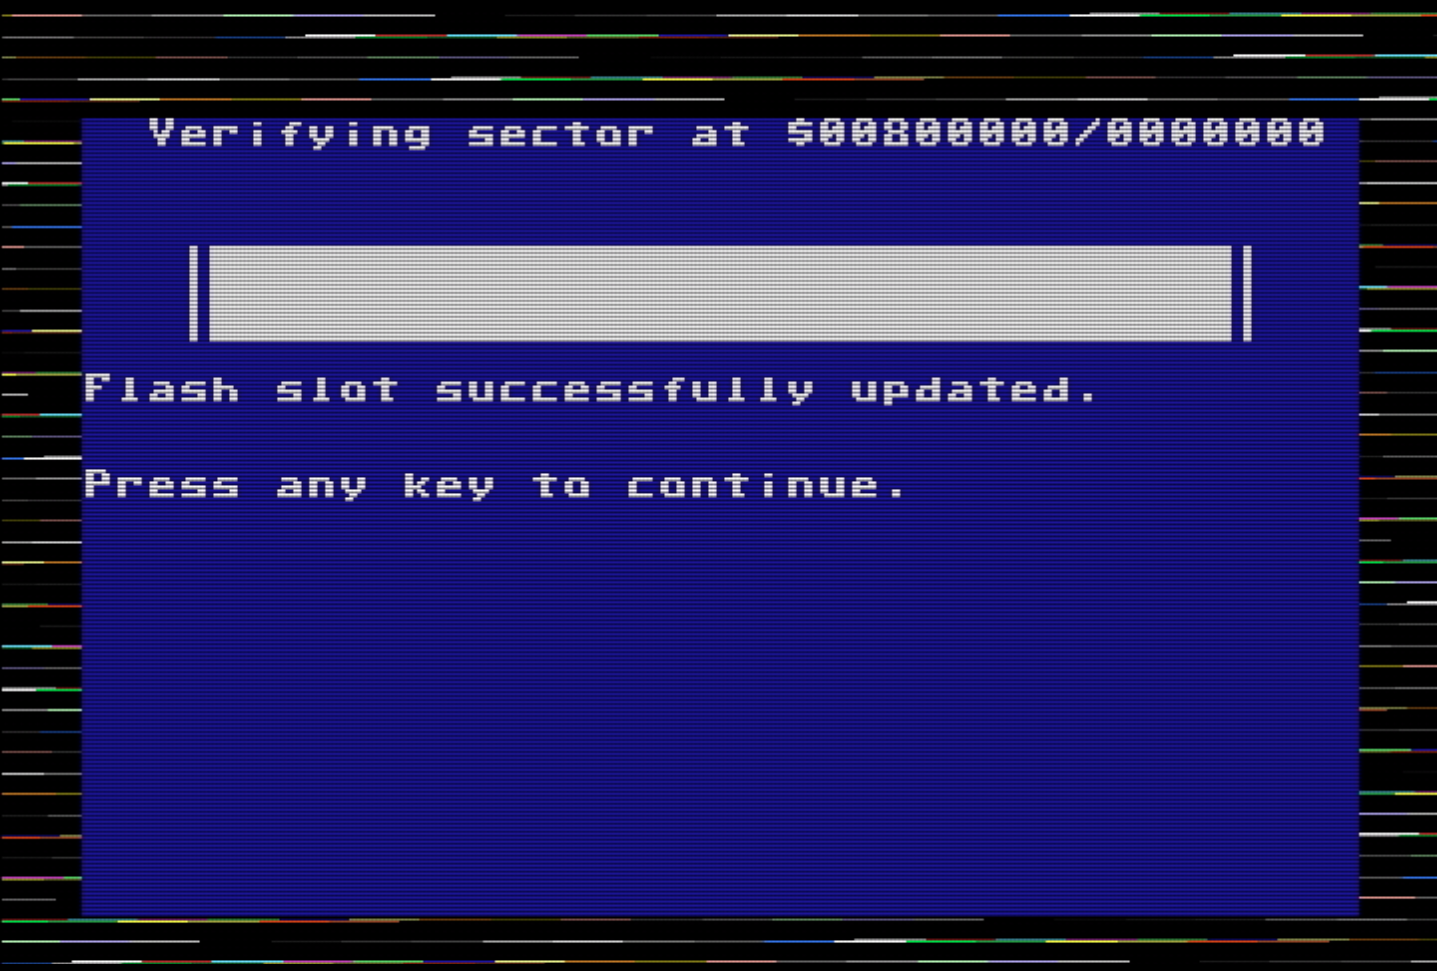
\includegraphics[width=0.7\linewidth]{images/ss-flashmenu-done.png}
\end{center}

It is now safe to switch off your computer. Press any key to return to the core selection menu, or switch the computer off then on again to start the default core.


\section{Installing Alternate Cores}

Installing an alternate core, such as the C64 core, uses the same steps for flashing the core to a slot.

It is recommended to use slots 2 through 7 for alternate cores, and reserve slot 1 for the latest MEGA65 core. Of course, there is nothing stopping you from installing an alternate core in slot 1, so that the MEGA65 behaves as a different type of computer when you switch it on. You can always choose the MEGA65 core from the core selection menu.


\newpage

\section{Upgrading the Factory Core in Slot 0}

It is possible to upgrade the factory-installed MEGA65 core in slot 0. You only need to do this in rare cases, such as if a newer version of the MEGA65 core includes changes or bug fixes for the start-up process. The process is elaborate, delicate, and could result in a MEGA65 that fails to start if something goes wrong. It is {\em strongly} recommended that you do not upgrade slot 0 unless the announcement for the release suggests that you do so. Most MEGA65 core upgrades are fully functional in slot 1.

{\em Please read these instructions carefully before starting the procedure.}

\begin{enumerate}
  \item Prepare to use the {\em internal SD card only}. This may involve opening the case to make the SD card easier to access. Do {\em not} use the external microSD card slot for updating core slot 0.
  \item Using your PC, rename the core file that you wish to install to this exact filename: {\tt UPGRADE0.COR} (That's the word {\tt UPGRADE}, the number zero, and {\tt .COR}, using uppercase letters.)
  \item Install the latest MEGA65 core in slot 1, using the procedure described earlier. The core must be in the default non-zero slot to recover from any problems when updating slot 0. Boot this core to test that it works.
  \item Open the core selection menu. Press \megasymbolkey and the comma key to start the flash procedure for slot 0. (You will not be prompted for a filename.)
\end{enumerate}

\ifdefined\printmanual
\else
\underline{Note}: If you have a revision R3A MEGA65, have not previously upgraded slot 0, and \megasymbolkey and \megakey{,} does not start the procedure, you have an older slot 0 core that does not have this feature. You can work around this by restarting the core selection menu with slot 1. From the core selection menu, prepare to hold down \specialkey{NO\\SCROLL}, press the \megakey{1} key to boot into the core then immediately press and hold \specialkey{NO\\SCROLL}. The core selection menu re-opens using slot 1. Press \megasymbolkey and the comma key to complete the slot 0 upgrade.
\fi

If something goes wrong during the slot 0 flashing process, your MEGA65 may not start correctly. Before doing anything else, switch on your MEGA65, and wait a minute or so. It should notice that there is no valid core in slot 0, then proceed to start the core in slot 1. You can hold \specialkey{NO\\SCROLL} during this to open slot 1's core selection menu and restart the flashing process.

If the MEGA65 cannot boot any core after several minutes, it may be stuck. You may be able to recover using a device known as a ``JTAG interface'' that connects your PC to the MEGA65 main board. This allows you to inject a bitstream directly into the FPGA. The part is inexpensive but not always available. Contact the MEGA65 team for assistance.


\newpage

\phantomsection
\section{Understanding The Core Booting Process}

This section summarises how the MEGA65 selects which core to start with when it is switched on.
The process is shown in the following figure:

\includegraphics[width=\linewidth]{images/illustrations/flashmenu-flowchart.pdf}

The booting process is governed by two facilities:
\begin{itemize}
  \item The Hypervisor (also known as HYPPO), which operates at a level above the kernel. One of its responsibilities is to manage aspects of the boot process. For more details on the Hypervisor, refer to
\ifdefined\printmanual
the {\bf MEGA65 Book}.
\else
 \bookvref{sec:hypervisor-mode}.
\fi
    In the diagram, activities performed by the Hypervisor have been highlighted in green.
  \item The core selection menu program (also known as MegaFlash), which provides a list of available core slots to choose from. In the diagram, activities performed by MegaFlash have been highlighted in blue.
\end{itemize}

When the MEGA65 is switched on, it does the following:
\begin{itemize}
\item Loads the bitstream stored in slot 0 of flash memory. If that is the MEGA65 Factory Core, the MEGA65
  HYPPO Hypervisor starts.
\item If it is the first boot since power-on (which implies that you are running from slot 0), HYPPO starts the Flash Menu program (aka MegaFlash) -- but note that the Flash Menu in
      this mode may not show anything on the screen to indicate that it is running!
\item The Flash Menu then checks if \specialkey{NO\\SCROLL} is being held down.
\item If it is, the Flash Menu program shows its display, allowing you to select or re-flash a core.
\item If \specialkey{NO\\SCROLL} is {\em not} being held down, the Flash Menu program checks if Flash Slot 1 contains a valid
      core.
\item If it does, then the Flash Menu program attempts to load that core.
\item If it succeeds, then the system reconfigures itself for that core, after which the behaviour of the system is
      according to that core.
\item If it fails, the keyboard will go into ``ambulance mode'', showing flashing blue lights to indicate that some
      first-aid is required. Note that in ambulance mode the reset button has no effect: You must switch the
      MEGA65 off and on again.
\end{itemize}

If you have selected a different core in the Flash Menu, the process is similar, except that the ambulance lights will appear for only a limited time, as the FPGA will automatically search through the flash memory until it finds a valid core. If it gets to the end of the flash memory, it will start the MEGA65 Factory Core from slot 0 again.

\chapter{Using Disks and Disk Images}
\label{cha:using-disks}

\phantomsection

\section{Disk Drives}
\index{Disk Drives}

The MEGA65 has a built-in 3.5" floppy disk drive, and supports Commodore-style external disk drives via the IEC serial port on the back of the computer. The IEC port also supports other external IEC storage devices, such as the SD2IEC. Some IEC storage devices can be connected in a chain and used at the same time.

The MEGA65 also includes a ``virtual'' disk drive that can mount D81 disk image files stored on the SD card. Most MEGA65 software that you download from the Internet is in the form of a D81 disk image. You can create a new D81 disk image directly from the MEGA65, and start saving your BASIC programs to the SD card without any additional hardware. You can also copy files between physical floppy disks and D81 disk images.

The Intro Menu that you saw when you first switched on the computer is a program on a D81 disk image, a file named {\tt MEGA65.D81} on the SD card. The MEGA65 is initially configured to boot this disk image automatically. You can change this in the Configuration Utility. (Refer back to chatper \vref{cha:configuringyourmega}.)

You can manage disk drives and virtual disk images from the Freezer menu. Some of these operations can be performed with BASIC commands such as {\bf MOUNT}.

\subsection{Unit Numbers and Drive Numbers}
\index{Disk Drives!Terminology}
\index{Connections!IEC}

Each disk drive (physical or virtual) is accessed via a {\it unit} number. With vintage Commodore computers, the unit number refers to an IEC device connected to the computer. Commodore reserved unit numbers in the range 0 -- 31 for devices of various purposes, with 8 -- 11 reserved for disk drives. If you've ever used a Commodore 64 and typed \screentext{LOAD "*",8,1}, the ``8'' refers to the disk drive connects as unit 8. BASIC 65 disk commands use unit 8 by default, and accept a {\bf U} parameter to change it, such as: \screentext{DLOAD "MYPROGRAM",U9}

With the MEGA65, you can assign a unit number to the virtual disk drive with a D81 disk image mounted, or to the internal 3.5" floppy drive. You must mount a disk image or the internal 3.5" floppy drive to a unit number before it can be used. Any message sent to a unit number assigned to a virtual disk or the internal floppy drive is handled by the MEGA65. All other messages are sent to the IEC serial port.

Disk commands also accept an optional parameter to specify a {\it drive} number. This is only needed when connecting a vintage dual floppy drive via the IEC port, such as the Commodore 4040, 8050, or 8250. Every disk drive assigns drive number 0 to the first drive. Dual-drive units assign a drive number of 1 to the second drive. Dual disk drives are usually equipped with an IEEE-488 interface, and need an IEEE-488 to IEC converter to be used on the MEGA65. BASIC 65 disk commands use device 0 by default, and accept a {\bf D} parameter to change it.


\section{Using Virtual Disk Images}

The MEGA65 provides a virtual disk drive that uses D81 disk image files from the SD card. The virtual drive behaves like a Commodore 1581 drive, without the need for vintage physical media.

You can mount up to two virtual disks at a time, or one virtual disk and the internal 3.5" floppy drive. Each virtual disk can be assigned to unit 8 or 10, and 9 or 11.

\subsection{Where to Get Disk Image Files}

The MEGA65 Filehost website hosts a library of MEGA65 software produced by the community. You can browse or search for software, download a title, then copy the D81 disk image to the SD card using either your PC or the Ethernet file transfer tool.

\url{https://files.mega65.org/}

\subsection{Mounting Disk Images with the Freezer}

Open the Freezer menu: hold \widekey{RESTORE} for one second, then release it. Notice the current drive mounting settings in the lower-right of the screen.

\begin{center}
  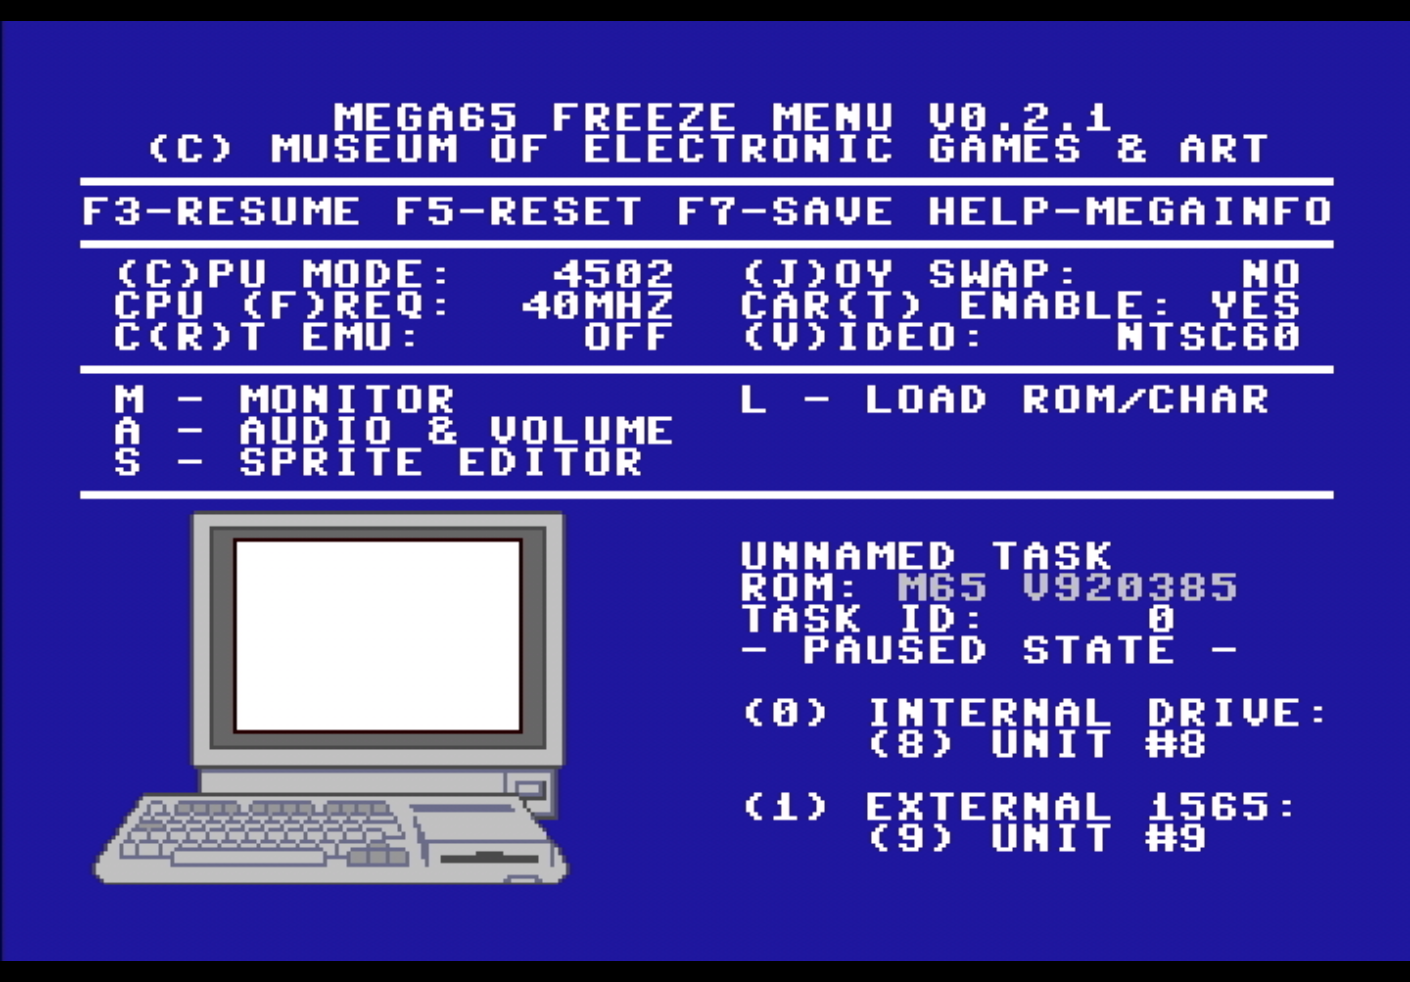
\includegraphics[width=0.7\linewidth]{images/freezer.png}
\end{center}

To mount a disk image on unit 8 or 10, select the first managed drive by pressing \megakey{0}. To mount a disk image on unit 9 or 11, select the second managed drive by pressing \megakey{1}. This opens the SD card file browser.

\begin{center}
  \includegraphics[width=0.7\linewidth]{images/d81-file-browser.png}
\end{center}

Use the cursor keys to select a D81 disk image, then press \widekey{RETURN}. The Freezer screen shows the selected disk image is now associated with the managed drive.

From the main Freezer screen, press \megakey{8} or \megakey{9} to toggle the unit number assigned to the first or second managed drive, respectively.

\subsection{Mounting Disk Images from BASIC}

The BASIC {\bf MOUNT} command can mount a D81 disk image from the SD card without having to open the Freezer. This command can be entered at the \screentext{READY} prompt, or be used as part of a program.

To mount a disk image on unit 8, enter {\bf MOUNT} with the full filename in double-quotes, including the {\tt .D81} suffix:

\begin{screenoutput}
MOUNT "MEGA65.D81"
\end{screenoutput}

To mount a disk image to unit 9, 10, or 11, also provide the {\bf U} argument:

\begin{screenoutput}
MOUNT "MEGA65.D81",9
\end{screenoutput}

\subsection{Creating a New Disk Image}

You can create a new empty disk image from within the MEGA65 Freezer.

\begin{enumerate}
\item Open the Freezer.
\item Press \megakey{0} to select the first managed drive.
\item At the top of the file list, select: \screentext{- NEW D81 DD IMAGE -}
\item When prompted, enter a name for the disk. (Omit the {\tt .D81} suffix; this will be added automatically.)
\end{enumerate}

The new disk image is created on the SD card and mounted to the first managed drive. It is formatted and ready to use.

\subsection{Managing SD Card Files in Sub-directories}

Once you have spent some time on Filehost downloading games and applications, you will eventually have a large collection of D81 disk images on your SD card. You may wish to organize these files into sub-directories (folders). You can create these folders with the SD card connected to your PC, or with the Ethernet file transfer tool.

The Freezer supports sub-directories in its file browser. Each sub-directory name begins with a slash (\screentext {/}). Select a folder to list it's files. To return to the previous folder, select \screentext {/...}

\begin{center}
  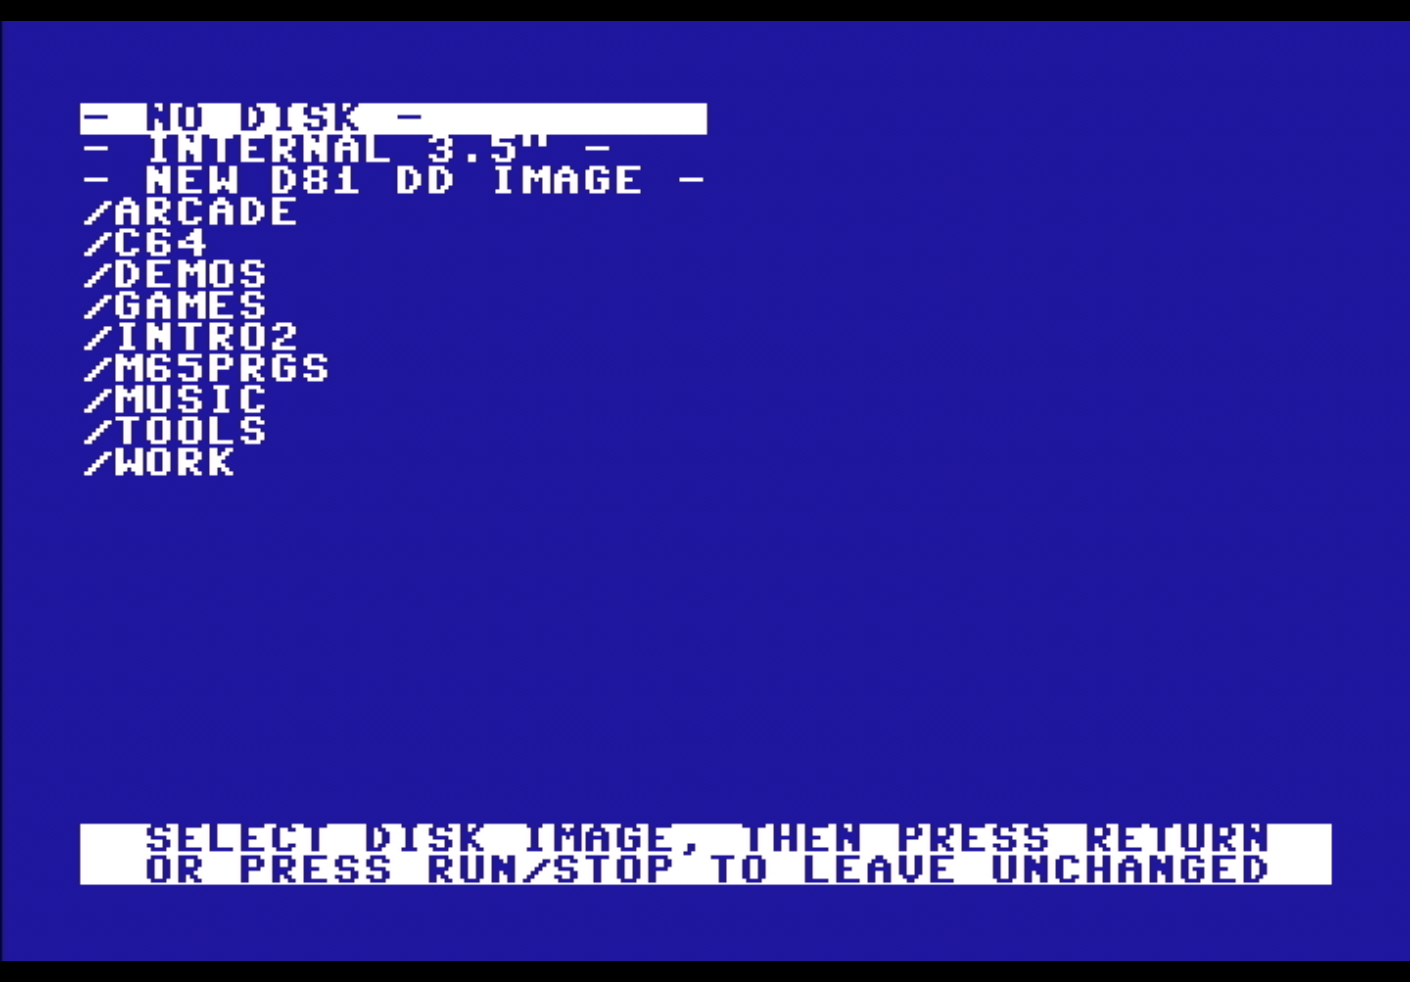
\includegraphics[width=0.7\linewidth]{images/d81-subfolders.png}
\end{center}

You can also create new disk images in sub-directories by navigating to the sub-directory before selecting \screentext{- NEW D81 DD IMAGE -}.

The MEGA65 maintains a ``current working directory'' that is used as the base directory for BASIC commands such as {\bf MOUNT}. To change the current working directory from BASIC, use the {\bf CHDIR} command with the {\bf U12} argument:

\begin{screenoutput}
CHDIR "DEMOS",U12

MOUNT "XANADU.D81"
\end{screenoutput}


\section{Using the Internal 3.5" Floppy Disk Drive}

The MEGA65 has a built-in 3.5" floppy disk drive, similar to what was intended for the Commodore 65. You can use physical floppy disks to store your programs and data. Some MEGA65 software can be purchased on floppy disk.

The internal 3.5" drive must be mounted before it can be used. It can be mounted to unit 8 or unit 10.

\subsection{Mounting the 3.5" Drive with the Freezer}

Open the Freezer menu: hold \widekey{RESTORE} for one second, then release it. Notice the current drive mounting settings in the lower-right of the screen.

Press \megakey{0}, then use the cursor down key to: \screentext{- INTERNAL 3.5" -} Press \widekey{RETURN} to select it. The Freezer menu screen shows that the internal drive is mounted to the first managed disk device.

The \screentext{UNIT \#} for the first device can be either 8 or 10. Press \megakey{8} to toggle between these options. BASIC disk commands default to unit 8, so it is typical to use unit 8 unless you are working with multiple disks at the same time.

The internal 3.5" drive cannot be mounted to the second managed drive with unit numbers 9 or 11.

\subsection{Mounting the 3.5" Drive from BASIC}

You can mount the internal 3.5" disk drive to unit 8 using the BASIC {\bf MOUNT} command. This command works from either the \screentext{READY} prompt or from a program. To mount the internal drive to unit 8, enter the command without arguments:

\begin{screenoutput}
MOUNT
\end{screenoutput}

The {\bf MOUNT} command can only mount the internal drive to unit 8. You can only mount it to unit 10 from the Freezer menu.

\subsection{DD vs. HD disks}

The MEGA65 disk controller expects a Double Density (DD) floppy disk in the internal 3.5" floppy disk drive.\footnote{It may be possible to support full-capacity HD disks in a future firmware update. This is not a limitation of the drive hardware.} Floppy disks are no longer manufactured, and the DD variety can be difficult to find.

You can use a High Density (HD) floppy disk with the drive, with one important modification: you must cover both sides of the hole in the upper-left corner (as seen from the front) of the disk with a small piece of tape. This convinces the drive that the disk is DD, and switches it to a mode compatible with the MEGA65 disk controller.

\begin{center}
  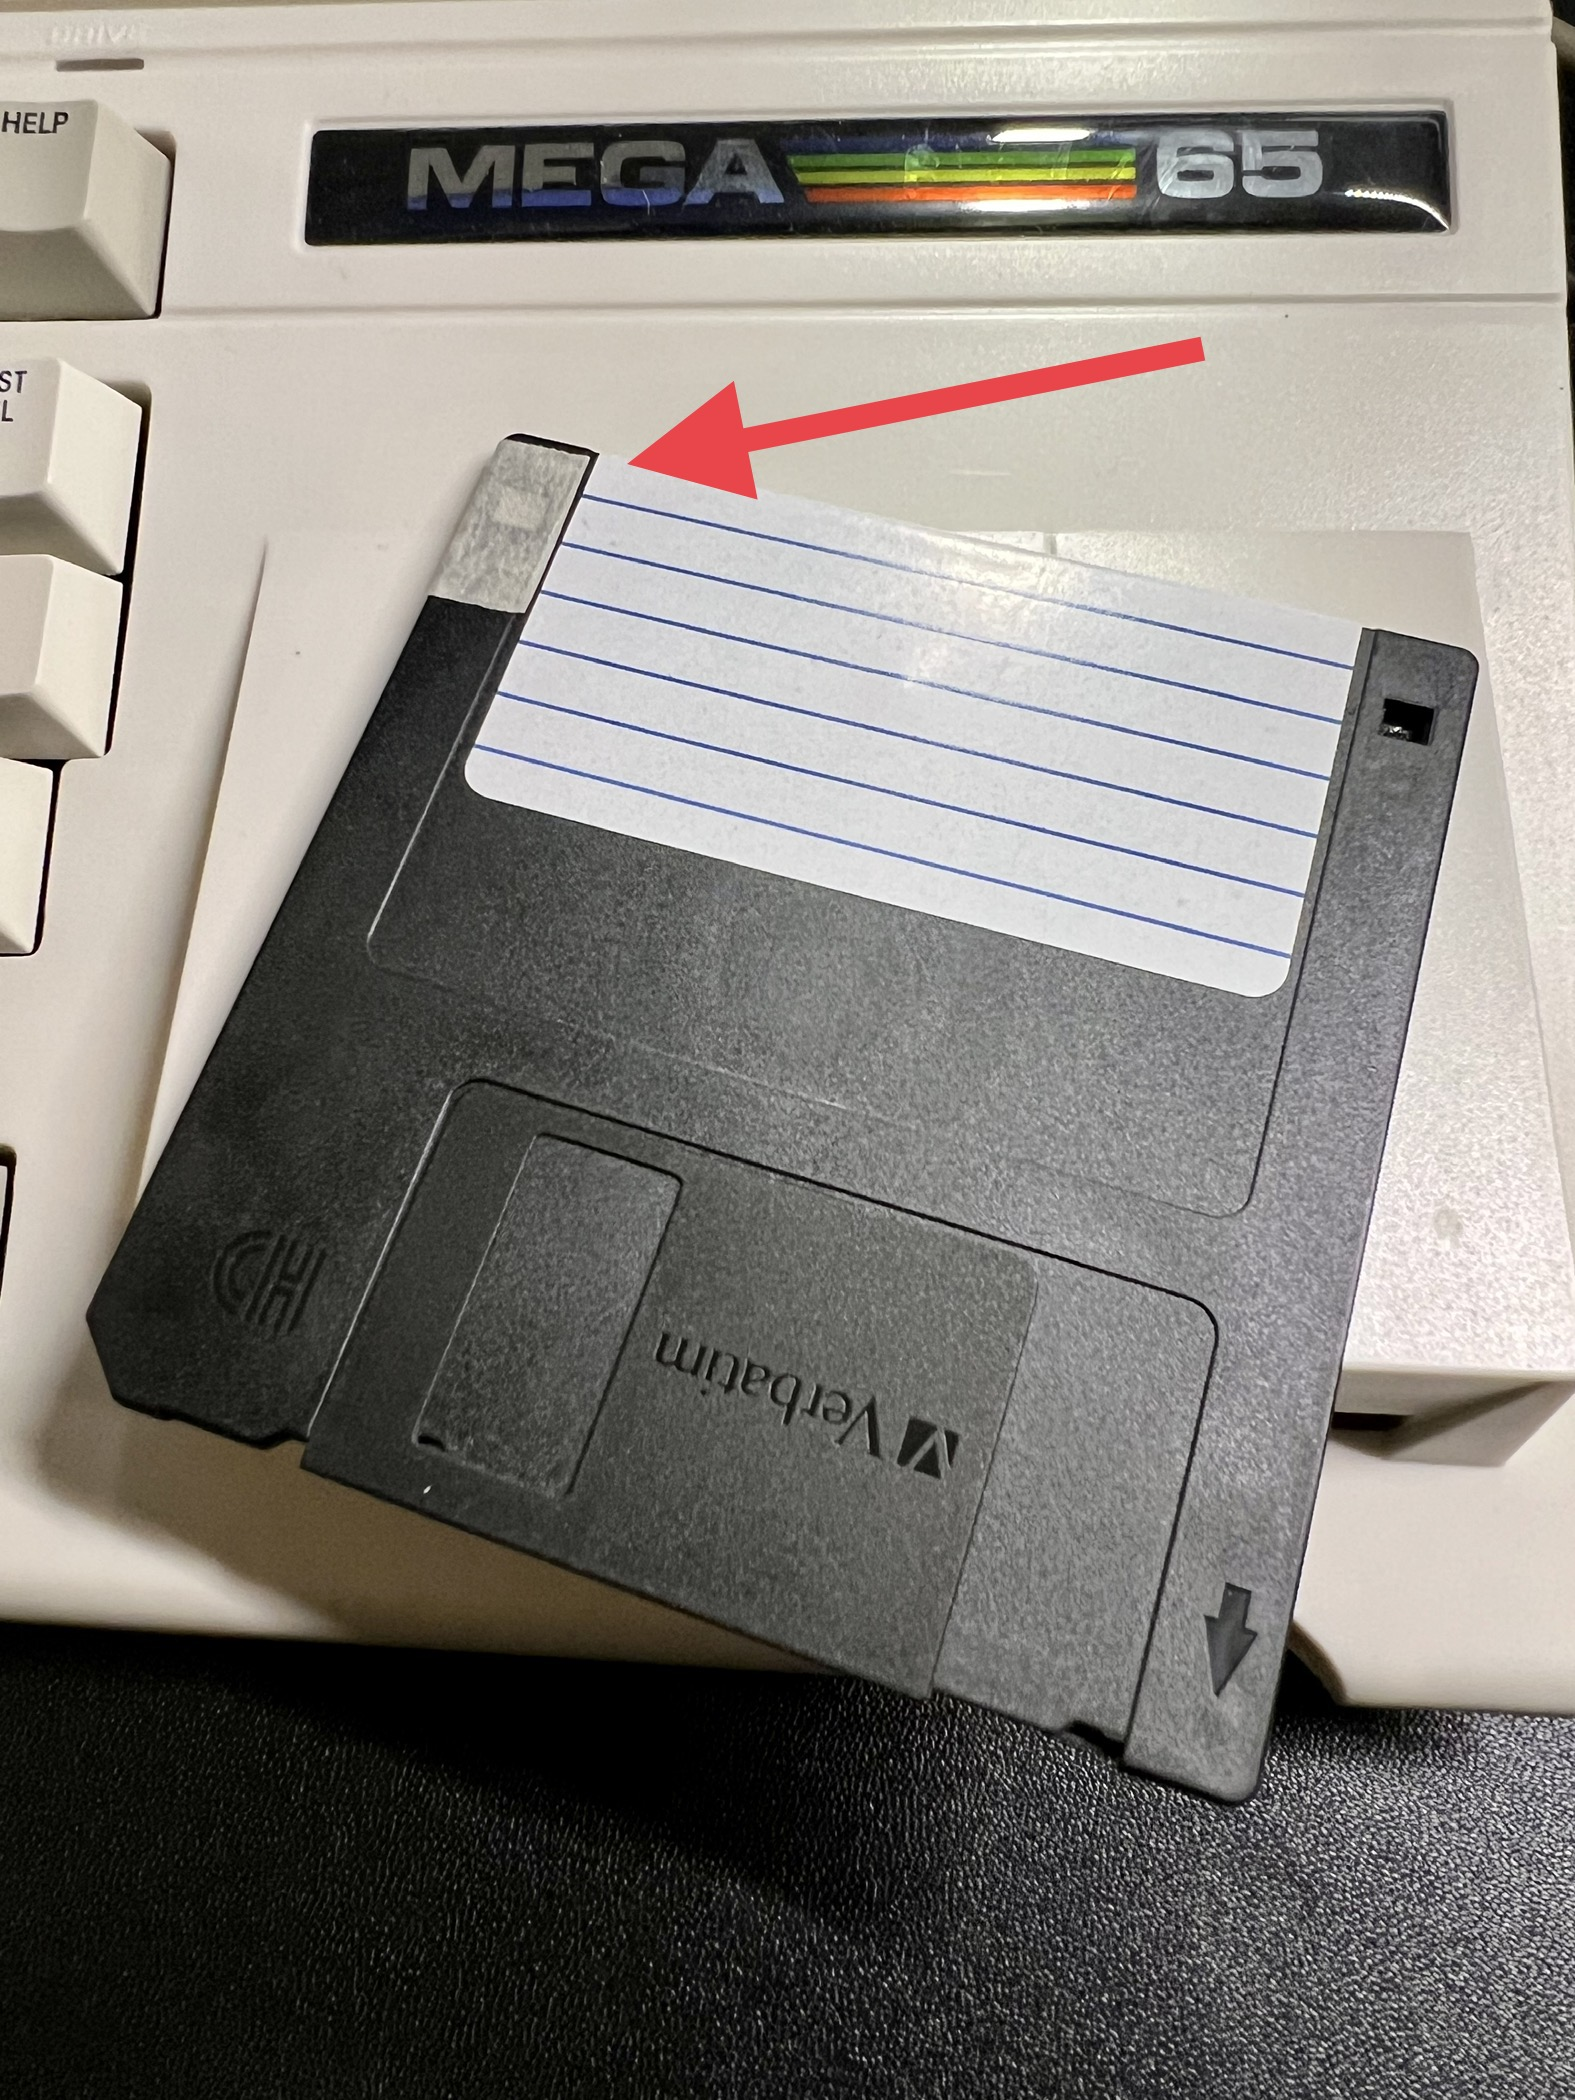
\includegraphics[width=0.7\linewidth]{images/floppy_hd.jpg}
\end{center}

\underline{Note}: Make sure that the tape covers both sides of the hole.

\subsection{Formatting a Disk}

A floppy disk must be formatted before it can be used. The MEGA65's internal 3.5" floppy drive emulates a Commodore 1581 drive, and can use disks formatted in such a drive. You can also format a disk with the MEGA65.

\underline{Note}: Formatting a disk erases its contents. Be careful to only do this when you do not need the data on the disk!

To format a physical 3.5" floppy disk using the internal drive:

\begin{enumerate}
\item Open the Freezer.
\item Mount the internal 3.5" floppy drive to the first managed drive slot, unit 8.
\item {\it Double-check that unit 8 says:} \screentext{- INTERNAL 3.5" -}
\item Resume the computer: press \megakey{F3}.
\item Insert the floppy disk you wish to format into the internal floppy drive.
\item Enter the BASIC {\bf FORMAT} command, giving it a name ({\tt "MYDISK"}) and a two-character ID ({\tt XX}).
\begin{screenoutput}
FORMAT "MYDISK",IXX
\end{screenoutput}
\item When prompted, enter {\tt YES} and press \widekey{RETURN}.
\end{enumerate}

Formatting the disk takes a minute or so. The drive will make buzzing and clicking noises during the process. Do not switch off the computer or eject the disk until formatting is complete.

You can confirm that the formatting was successful by issuing the {\bf DIR} command. You should see an empty directory listing with the name and ID you specified. Your disk is now ready to use.


\section{Using External IEC Disk Drives}

The MEGA65 works with external disk drives connected to the IEC serial port.

External drives do not need to be mounted. If a unit number is not assigned to the internal 3.5" disk drive or to a disk image, disk operations intended for that unit number will be transmitted to the IEC serial port. It is up to the device connected to the port to recognize its unit number. Some IEC devices have switches that let you set the unit number. Others will only work with a specific number.

If you have an external drive that expects a specific unit number, you will need to make sure the MEGA65 isn't assigning that number to a disk image or the internal drive. Open the Freezer, then press \megakey{8} or \megakey{9} to toggle the unit number assignments so that they no longer use the needed unit number.

The drive and unit assignments are temporary, and will be reset to their defaults when the MEGA65 is switched off. You will need to re-configure the drive assignments the next time you switch on the computer.


\section{Bootable Disks}

With older Commodore computers, it was common for software makers to organize the file directory on a floppy disk such that the first file in the list is the main program. The user could then enter the command \screentext{LOAD "*",8,1} to load the main program, and \screentext{RUN} to run it. The asterisk is a wildcard that matches any file, so it matches the first file on the disk, without the user having to type the name of the program.

This method is still common, and the MEGA65 has a quick way to boot such disks: hold \specialkey{SHIFT} and press \specialkey{RUN STOP}. This executes the \screentext{RUN "*"} command, which is similar to the familiar command sequence that loads and runs the first program on the disk.

With the C65, Commodore introduced a new way to boot disks. Instead of relying on file order, a disk can have a file named {\tt AUTOBOOT.C65}. If this file exists and is a program, the BASIC {\bf BOOT} command will load and run this file.

\begin{screenoutput}
BOOT
\end{screenoutput}

\subsection{Auto-Booting Disks}

As discussed in chapter \vref{cha:configuringyourmega}, you can use the Configuration Utility to set the MEGA65 to mount either a virtual disk image or the internal 3.5" disk drive automatically during boot. (You can also disable this feature by selecting the virtual disk, then leaving the field that asks for the disk image name empty.)

If the mounted disk is bootable --- that is, it contains a program file named {\tt AUTOBOOT.C65}, the MEGA65 will load and run the boot program automatically.

This is how the Intro Disk works. The Intro Disk menu is a program named {\tt AUTOBOOT.C65} on the virtual disk image {\tt MEGA65.D81}, which is pre-configured to be the mounted disk on system start-up. When you disable the Intro Disk from its menu, it renames {\tt AUTOBOOT.C65} to {\tt MENU}, such that the disk is no longer considered bootable.

Setting up a boot disk for yourself can be a handy way to configure your computer. You can write a short BASIC program that changes the system font, adjusts the background color, and sets {\bf KEY} macros to your taste, then save the program as {\tt AUTOBOOT.C65} on a disk that you have configured to mount on system start-up. This program will run every time you switch on your MEGA65.


\section{Accessing the SD Card from BASIC}

Several BASIC 65 commands can operate directly on the MEGA65 SD card as if it were a disk drive. In these cases, the SD card is known as unit 12.

\underline{Note}: Unit 12 can only be accessed directly for a few specific operations. It cannot treat the entire SD card as if it were a CBDOS disk.

To list all of the files on the SD card, use the {\bf DIR} command with the \screentext{U12} argument:

\begin{screenoutput}
DIR U12
\end{screenoutput}

To load or save a PRG file directly from the SD card (that isn't in a D81 disk image), use the \screentext{U12} argument with the {\bf DLOAD} and {\bf DSAVE} commands. You {\em must} include the {\tt .PRG} filename suffix in this case, which is different from using PRG files on disks or disk images.

\begin{screenoutput}
DLOAD "MYPROGRAM.PRG",U12
\end{screenoutput}

As shown earlier, the MEGA65 supports sub-directories (sub-folders) on the SD card, and maintains a current working directory for disk operations. To change the current working directory to a subdirectory:

\begin{screenoutput}
CHDIR "SUBDIR",U12
\end{screenoutput}

To change the current working directory to the parent of the current directory:

\begin{screenoutput}
CHDIR "..",U12
\end{screenoutput}

The {\bf MOUNT} command can mount a D81 disk image to a unit number. Even though this command refers to a file on the SD card, it does not use the \screentext{U12} argument. Instead, it uses the {\bf U} argument to select the unit number for the disk being mounted. The {\bf MOUNT} command uses the current working directory set by {\bf CHDIR} to locate the file.


\section{Common Disk Operations}

The following are some examples of common disk operations you can perform at the \screentext{READY} prompt. See the BASIC command reference in appendix \vref{cha:basic-reference} for more information.

Most commands that accept filenames also accept a {\bf U} argument that says which unit has the file. The default unit is 8.\footnote{The default disk unit for BASIC commands is 8. You can change it with the {\bf SET DEF} command.}

\subsection{DIR}

To display the directory (list of files) for a disk, use the {\bf DIR} command.

\begin{screenoutput}
DIR

DIR U9
\end{screenoutput}

Unlike the Commodore 64 method of loading the disk directory into BASIC memory, the {\bf DIR} command does not modify BASIC memory. It is safe to use {\bf DIR} with a program in memory.

To make larger directories easier to view, {\bf DIR W} (for ``wide'') displays the directory in columns, pausing for each page.

\subsection{DLOAD and RUN}

The {\bf DLOAD} command loads a program from disk into memory. The {\bf RUN} command runs the program currently in memory.

\begin{screenoutput}
DLOAD "COOLGAME"
RUN
\end{screenoutput}

You can combine these into one command by providing the filename directly to the {\bf RUN} command.

\begin{screenoutput}
RUN "COOLGAME"
\end{screenoutput}

\subsection{DSAVE}

The {\bf DSAVE} command saves the BASIC program currently in memory to disk.

\begin{screenoutput}
DSAVE "MYGAME"
\end{screenoutput}

By default, this will not overwrite an existing file with the same name. To request that the existing file be overwritten, insert an {\tt @} (at) symbol before the filename, inside the double-quotes.

\begin{screenoutput}
DSAVE "@MYGAME"
\end{screenoutput}

Note that save-with-replace is only recommended when using disk images and the 3.5" floppy drive. Older Commodore drives have bugs in this feature that could result in data loss.

\subsection{BACKUP}

The {\bf BACKUP} command copies an entire disk from one unit to another. All existing data on the destination disk is erased as part of this process.

\begin{screenoutput}
BACKUP U8 TO U9
\end{screenoutput}

You can use {\bf BACKUP} to make disk images from floppy disks, or write disk images to floppy disks, or copy everything from one disk drive to another.

\subsection{COPY}

The {\bf COPY} command makes a copy of a file. If the source and the destination are different filenames on the same unit, this duplicates the file on the disk.

\begin{screenoutput}
COPY "MYGAME",U8 TO "MYGAME",U9

COPY "MYGAME" TO "MYGAME-V1"
\end{screenoutput}

\subsection{RENAME}

The {\bf RENAME} command changes the name of an existing file.

\begin{screenoutput}
RENAME "MYGAME-V29" TO "MYGAME-FINAL"
\end{screenoutput}

\subsection{DELETE}

The {\bf DELETE} command deletes a file.

\begin{screenoutput}
DELETE "JUNKFILE"
\end{screenoutput}


\subsection{Shortcut Disk Commands}

BASIC 65 provides several shortcuts for common disk commands for use from the \screentext{READY} prompt.

\begin{center}
\begin{tabular}{|l|l|}
\hline
{\bf Shortcut} & {\bf Equivalent Command} \\
\hline
\screentextwide{/} & {\bf LOAD} \\
\hline
$\uparrow$ & {\bf RUN} \\
\hline
$\leftarrow$ & {\bf SAVE} \\
\hline
\screentextwide{@} & {\bf DISK} \\
\hline
\screentextwide{\$} & {\bf DIR} \\
\hline
\end{tabular}
\end{center}

These are intended to be used with a directory listing to launch programs without having to type filenames. For example:

\begin{enumerate}
\item Display the disk's directory listing: type {\bf \$}, press \widekey{RETURN}.
\item Use the cursor keys to move the cursor to the line with the program you want to run.
\item Type {\bf \screentext{$\uparrow$}}, press \widekey{RETURN}.
\end{enumerate}

The selected program loads and runs. Notice that you do not have to clear extra characters from the line. The shortcut knows to ignore everything but the filename in double-quotes, as printed by the directory listing.


\part{FIRST STEPS IN CODING}

\input{howcomputerswork}
\input{beginninginbasic}
\input{text-processing}
\input{morebasic}
\input{datainbasic}
\input{modes}

\part{SOUND AND GRAPHICS}

\input{graphics}
\input{sprites}
\input{sound}

\part{MEMORY}

\input{memory}

\part{HARDWARE}

\chapter{Using Nexys4 boards as a MEGA65}

\section{Building your own MEGA65 Compatible Computer}

You can build your own MEGA65-compatible computer by using either a Nexys4DDR (aka. Nexys A7) or the older Nexys4 (Non-DDR) FPGA development boards.
This appendix describes the process to set up a Nexys4DDR (Nexys A7) board for this purpose (which is the newer, preferred board).
The older non-DDR Nexys4 board is also supported, and the instructions are the same, except that
you must use a bitstream designed for that board.
Using a Nexys4DDR bitstream on a non-DDR Nexys4 board, or vice versa, may cause irreparable damage to your board, so make sure
you have the correct bitstream to suit your board.


DISCLAIMER: M.E.G.A cannot take any responsibility for any damage that may occur to your Nexys4DDR/NexysA7/Nexys4 boards.

\newpage

\section{Working Nexys4 Boards}

There are currently 3 Nexys FPGA boards which can be setup as a MEGA65:

\begin{minipage}{\linewidth}
  \subsection{The Nexys4 board}

  No longer manufactured but still available for sale on some websites with old stock.

  \begin{center}
    \includegraphics[width=0.4\linewidth]{images/img001_nexys4_board.jpg}
  \end{center}

  Documentation:

  \begin{itemize}
    \item \url{https://reference.digilentinc.com/reference/programmable-logic/nexys-4/reference-manual}
    \item \url{https://reference.digilentinc.com/\_media/reference/programmable-logic/nexys-4/nexys4\_rm.pdf}
  \end{itemize}
\end{minipage}

\begin{minipage}{\linewidth}
  \subsection{The Nexys4DDR board}

  No longer manufactured but still available for sale on some websites with old stock.

  \begin{center}
    \includegraphics[width=0.4\linewidth]{images/img002_nexys4_ddr_board.jpg}
  \end{center}

  Documentation:

  \begin{itemize}
    \item \url{https://reference.digilentinc.com/reference/programmable-logic/nexys-4-ddr/reference-manual}
    \item \url{https://reference.digilentinc.com/\_media/reference/programmable-logic/nexys-4-ddr/nexys4ddr\_rm.pdf}
  \end{itemize}
\end{minipage}

\begin{minipage}{\linewidth}
  \subsection{The Nexys A7}

  This is the re-branded version of the above Nexys4 DDR board:

  \begin{center}
    \includegraphics[width=0.4\linewidth]{images/img003_nexysA7_board.jpg}
  \end{center}

  Documentation:

  \begin{itemize}
    \item \url{https://reference.digilentinc.com/reference/programmable-logic/nexys-a7/reference-manual}
    \item \url{https://reference.digilentinc.com/\_media/reference/programmable-logic/nexys-a7/nexys-a7\_rm.pdf}
  \end{itemize}
\end{minipage}

\newpage

\section{Power, Jumpers, Switches and Buttons}

This top-down picture highlights the key jumper positions of interest on the Nexys4 board:

  \begin{center}
    \includegraphics[width=0.9\linewidth]{images/nexys4_jumpers.png}
  \end{center}

The Nexys4 boards can be powered in two ways: using an external power supply, or from a standard USB port.

\subsection{Micro-USB Power}

\includegraphics[width=5cm]{images/illustrations/nexys-micro-usb-power.pdf}

Connect your micro-usb cable to a USB port on a USB charger or PC to provide power. Connect the other end to the Nexys4's micro-usb connector. Place the JP3 jumper on pins 1 and 2 to select USB power. Use the switch to power up the Nexys4.

\subsection{External Power Supply}

\hspace*{1.7cm}
\includegraphics[width=3.2cm]{images/illustrations/nexys-power-supply.pdf}

The MEGA65 core can consume a lot of power, and a standard USB port could potentionally be too little for the Nexys4 board. In particular, writing to the SD card might hang or perform odd behaviour. Therefore you should consider a 5V power supply.

Digilent sell a power supply for the Nexys4 board, and we recommend you use this to ensure you avoid the risk of damage to your Nexys4 board. The chosen power supply should be center positive, 2.1mm internal diameter plug, and should deliver 4.5VDC to 5.5VDC rated at least 1 Amp.

Connect the power supply cable to the supply plug of the Nexys4. Place the JP3 jumper on pins 2 and 3 to select WALL power. Use the switch to power up the Nexys4.

\subsection{Other Jumpers and Switches}

For your initial set up, we'd suggest you set the following jumpers on your Nexys4 board to these positions:

\begin{itemize}
  \item{JP1} - USB/SD
  \item{JP2} - SD
\end{itemize}

\begin{center}
  \includegraphics[width=3.2cm]{images/illustrations/nexys-jumpers.pdf}
\end{center}

This will assure that the bitstream files will get loaded from your SD card on start-up.

At some later stage, you may prefer to load the bitstream from the on-board QSPI flash, and at that point, you can revisit your JP1 jumper setting and adjust it to the QSPI position.

% XXX - Image of board highlighting the jumpers

All 16 switches on the lower edge of the board must be set to the off position.


\subsection{Connections and Peripherals}

\includegraphics[width=\linewidth]{images/illustrations/nexys-connectors.pdf}

A USB keyboard can be connected to the USB port. Only a keyboard that lacks a USB hub will work with the Nexys4 board.  Generally, extremely cheap keyboards will work, while more expensive keyboards tend to have a USB hub integrated, and will not work.  You may need to try several keyboards before you find one that works.

You can connect a VGA monitor to the VGA port.

The mono audio-out jack can be connected to the line-in of an amplifier.


\subsection{Communicating with your PC}

There may be occasions where you wish to communicate with your Nexys4 board from your PC, in order to perform activities such as:

\begin{itemize}
  \item Flash your QSPI flash chip via Vivado
  \item Upload bitstream files directly from your PC (via m65 tool)
  \item Make use of support tools such as M65Connect, m65, mega65\_ftp, m65dbg, etc
\end{itemize}

On such occasions, you will need to connect your micro-usb cable up to your PC.

\includegraphics[width=5cm]{images/illustrations/nexys-micro-usb-power.pdf}

\subsection{Onboard buttons}

\begin{center}
  \includegraphics[width=3.2cm]{images/illustrations/nexys-reset-buttons.pdf}
\end{center}

The ``CPU RESET'' button will reset the MEGA65 when pressed, while the ``PROG'' button will cause the FPGA itself to reload the MEGA65
core.  The main difference between the two is that CPU RESET is faster, and does not clear the contents of memory, while the FPGA button
is slower, and does reset the contents of memory.

\begin{center}
  \includegraphics[width=3.2cm]{images/illustrations/nexys-five-buttons.pdf}
\end{center}

Two of the five buttons in the cross arrangement can also be used:  BTND acts as though you have pressed \widekey{RESTORE}, while BTNC will trigger an IRQ, as though the IRQ line had been pulled to ground.

\section{Keyboard}

The keyboard layout is positional rather than logical.
This means that keys in similar positions to the keys on a C65 keyboard will have similar function.
This relationship assumes that your USB keyboard uses a US keyboard layout.

To help you locate what the various MEGA65 keys are mapped to, the MEGA65 has a built-in virtual keyboard test feature. This can be accessed in two ways.

The easiest way is to keep \specialkey{ALT} held down in while switching on the Nexys4, or resetting the Nexys4 with
the ``PROG'' button. The configure menu will be presented and by pressing 3, the virtual keyboard will be presented on a black background.

\includegraphics[width=\linewidth]{images/illustrations/virtual-keyboard.pdf}

Pressing a key on the USB keyboard will show the highlighted key on the virtual keyboard to help you identify the key mapping.

The other way to access the virtual keyboard is from within the MEGA65. Hold \megasymbolkey and press \specialkey{TAB} to access the Matrix Mode Debugger. From here, enter the following:

\screentextwide{s ffd3615 ff}

This will open a semi-transparent virtual keyboard at the top of the screen. Alternatively:

\screentextwide{s ffd3615 ff ff}

This will open a semi-transparent virtual keyboard in the centre of the screen.

Hold \megasymbolkey and press \specialkey{TAB} to exit Matrix Mode Debugger and return to the MEGA65.

\subsection{Some key mappings with a USB keyboard}

\widekey{RESTORE} is mapped to the PAGE UP key.

\specialkey{RUN STOP} is mapped to \specialkey{ESC}.

\newpage

\section{Preparing microSDHC card}

The MEGA65 requires an SDHC card of between 4GB and 64GB capacity.  Some SDXC cards may work, however, this is not officially supported.

Preparation steps for the Nexys4 board's SD card share much in common with the
steps needed for real MEGA65 hardware, and as such, it is worth having a look
over
\ifdefined\printmanual
the {\bf MEGA65 Book}
\else
\bookvref{cha:configuringyourmega}
\fi
if you ever need details.

So in this section, we'll provide more details on the distinctive steps, and be more brief on the common steps.

One point of distinction between the Nexys board and the real MEGA65 hardware is that the latter already has a default bitstream/core provided, which permits you to format your SD card in the specific style required by the MEGA65.

For Nexys4 board owners however, you have no such default bitstream, so
see
the {\bf MEGA65 Book}
for more details on where the appropriate "nexys4.bit" or "nexys4ddr-widget.bit" files for your device can be downloaded from.

\subsection{Preparation Steps}

The steps are:

\begin{itemize}
  \item{Format the SD card} in a convenient computer using the FAT32 file-system.  The MEGA65 and Nexys4 boards do not understand other
file systems, especially the exFAT file system.
\item{Copy} your bitstream file (with name ending in ``.bit'') onto the SD card.
\item{Insert} the SD card into the SD card slot on the under-side of the Nexys4 board.
\item{Switch on} the Nexys4 board.
\item{Enter the Utility Menu} by holding \specialkey{ALT} down on the USB keyboard you have connected to the Nexys4 board.
\item{Enter the FDISK/FORMAT tool} by pressing 2 when the option appears on the MEGA65 boot screen.
\item{Follow the prompts} in the FDISK/FORMAT program to again format the SD card for use by the MEGA65. \\
  \\
  The FDISK tool will partition your SD card into two partitions and format them.
  \begin{itemize}
    \item One is type \$41 = MEGA65 System Partition, where the save slots, configuration data and other files live. \\
  (This partition is invisible in i.e. Win PCs).
    \item The other partition with type \$0C = VFAT32, where KERNAL, support files, games, and so on, will be copied to later. \\
  (This partition is visible on i.e. Win PCs).
  \end{itemize}
\item{Once formatting is complete}, switch off the Nexys4 board and remove the microSDHC card from the Nexys board and put it back into your PC
\item{This time, copy} the following items onto the SD card:
  \begin{itemize}
    \item The bitstream file
    \item The extracted files from within either the "\textbf{SD essentials.rar}"
	      or "\textbf{SD essentialsNoROM.rar}" file that you downloaded from
		  the MEGA65 filehost. (See
\ifdefined\printmanual
the {\bf MEGA65 Book}
\else
\bookvref{sec:installingrometc}
\fi
		  for more details).
    \item{If you have sourced your own preferred ROM file} (e.g. "\textbf{911001.BIN}"), copy it onto the SD card also, and rename it to "\textbf{MEGA65.ROM}" (uppercase is essential).
    \item{Any .D81 disk image files} you wish to make use of.
      \begin{itemize}
        \item Note that if a file named MEGA65.D81 is added to the SD card, it will be mounted automatically on startup.
        \item Make sure that all .D81 files have names that fit the old DOS 8.3 character limit, and are upper case.  This restriction will be removed in a future release.
      \end{itemize}
  \end{itemize}
\item{Remove the SD card} and reinsert it into your Nexys4 board.
\item{Power the Nexys4} board back on.  The MEGA65 should boot within 15 seconds.
\item On first start up, you will find yourself at the on-boarding screen, of which more
    details can be found in
\ifdefined\printmanual
the {\bf MEGA65 Book}
\else
\bookvref{cha:configuringyourmega}
\fi
.

\end{itemize}

Congratulations. Your MEGA65 has been set up and is ready to use.

Please note that the above method of copying the bitstream file to the SD card means that the bitstream is loaded into the Nexys FPGA each time on boot - which takes around 13 seconds for the system to start. The bitstream can also be flashed using Vivado software into the QSPI flash to deliver a boot up time of 0.3 seconds.

For more detailed information on preparing and configuring your MEGA65, please refer
to
\ifdefined\printmanual
the {\bf MEGA65 Book}
\else
\bookvref{cha:configuringyourmega}
\fi
chapter.

\section{Loading the bitstream from QSPI}

While loading the bitstream from the SD card is the suggested (and well-trodden) path this document has chosen, of late, more nexys4 users have been exploring the alternative pathway of loading the bitstream from the QSPI flash. Some potential reasons they have chosen this pathway are:

\begin{itemize}
  \item Faster loading times (0.3 seconds versus 13 seconds)
  \item Some people were interested in the possibility of flashing multiple
        cores onto their QSPI (via steps described in the
\ifdefined\printmanual
the {\bf MEGA65 Book}
\else
\bookvref{cha:cores}
\fi
		Chapter)
  \item Some people have experienced niggling issues with the SD card pathway, such as:
    \begin{itemize}
      \item System unable to reboot from on-boarding screen
      \item System unable to reboot from freeze-menu after switching between PAL/NTSC
    \end{itemize}
\end{itemize}

In time, if this proves to be a more popular pathway, we can revise our documentation here to suit it. Here are some steps in brief.

\subsection{Preparation Steps}

For users that want to try this pathway, you will need to adjust the JP1 jumper setting to use QSPI and then follow the steps in the \nameref{cha:fpgacpldflashing} chapter in relation to \nameref{sec:installvivado} and \nameref{sec:mainfpgaflashing}.

Be forewarned that the installation of Vivado is a lengthy process (both in terms of download time, and installation time).

Once you have flashed Slot0 of your QSPI chip via Vivado, you can then follow the steps
described in
\ifdefined\printmanual
the {\bf MEGA65 Book}
\else
\bookvref{cha:configuringyourmega}
\fi
to perform the custom SD card formatting,
installing of ROM and support files and on-boarding.

\section{Widget Board}

For Nexys board owners (all models), you may be interested in adding a widget board to your nexys device, in order to allow you to connect to:

\begin{itemize}
  \item{a genuine C64 or C65 keyboard}
  \item{2 DB-9 joysticks}
  \item{Paddles or a 1351 Mouse}
  \item{Cartridges (not functioning as yet)}
\end{itemize}

The widget board connects to your nexys board via its PMOD connectors.

It presently is only available as an unpopulated PCB, purchasable from here:

\begin{itemize}
  \item \url{https://oshpark.com/shared\_projects/Y37xg9N7}
\end{itemize}

The firmware, pcb diagram, schematic diagram and bill of materials can be found within the following github project:

\begin{itemize}
  \item \url{https://github.com/sy2002/DM65PIC}
\end{itemize}

You will need to purchases parts from the bill of materials separately and populate the board yourself.

You may find this forum64.de thread of interest, if you would like to read on the experiences of others that undertook this process, or if you have questions of your own to ask:

\begin{itemize}
  \item \url{https://www.forum64.de/index.php?thread/90465-mega-65-ports-add-on-card-still-available-if-where}
\end{itemize}

The pcb (c65Keyb.brd) and schematic (c65Keyb.sch) files can be found within the 'eagle/' subfolder of the DM65PIC project, and can be viewed via the free tool 'AutoDesk Eagle', available here:

\begin{itemize}
  \item \url{https://www.autodesk.com/products/eagle/free-download}
\end{itemize}

Here are some photos of the widget board in use:
  \begin{center}
    \includegraphics[width=0.9\linewidth]{images/widget-board-martin.png}
  \end{center}
  \begin{center}
    \includegraphics[width=0.9\linewidth]{images/widget-board-deft1.png}
  \end{center}
  \begin{center}
    \includegraphics[width=0.9\linewidth]{images/widget-board-deft2.png}
  \end{center}

For convenience, the pcb and schematics diagrams for the widget board have also been provided in \bookvref{sec:nexyswidgetschematics}.

Some additional backstory notes for the board are:

\begin{itemize}
  \item{The widget board is originally meant to sit inside a c65 case}
  \item{Expansion port is not usable and a bit needs to be cut out for c64 case}
  \item{Would be reasonable to adapt it for c64 case use (which definitely will be the more regular use)}
\end{itemize}

\section{PMOD-to-Joystick Adaptor}

As an alternate (and cheaper) option for those that just want to add a DB9 joystick port via the PMOD connectors, a user from the community, TheChief, has devised a means to do so. More information can be found in the following Discord thread:

\begin{itemize}
  \item \url{https://discord.com/channels/719326990221574164/903079038015389716/929369283119685643}
\end{itemize}

  \begin{center}
    \includegraphics[width=0.9\linewidth]{images/joystick-pmod-thechief.png}
  \end{center}

\begin{minipage}{\linewidth}
\begin{center}
  \begin{longtable}{|L{3cm}|L{3cm}|p{3cm}|}
    \hline
    {\textbf{Joystick action}} & {\textbf{PMOD-JA Connections}} & {\textbf{DB9 Connections}} \\
    \hline
    {Fire} & {jahi(9)} & {pin 6} \\
    \hline
    {Up} & {jalo(1)} & {pin 1} \\
    \hline
    {Left} & {jalo(2)} & {pin 3} \\
    \hline
    {Down} & {jahi(7)} & {pin 2} \\
    \hline
    {Right} & {jahi(8)} & {pin 4} \\
    \hline
  \end{longtable}
\end{center}
\end{minipage}


\section{Useful Tips}

The following are some useful tips for getting familiar with the MEGA65:

\begin{itemize}

\item{Press \& hold \megasymbolkey (or the Commodore key if using a Commodore 64 or 65 keyboard) during boot to start up in C64-mode instead of C65-mode}
 \item{Press \& hold \specialkey{RUN STOP} during boot to enter the machine language monitor, instead of starting BASIC.}
\item{Press \widekey{RESTORE} for approximately 1/2 - 1 second to enter the MEGA65 Freeze Menu.  From this menu
  you have convenient tools to change the CPU speed, switch between PAL \& NTSC video mode, change Audio settings, manage freeze-states,
   select D81 disk images, examine and modify memory of the frozen program, among other features.  This is in many ways the heart of the MEGA65, so it is well worth exploring and getting familiar with.}
\item{Type \screentext{POKE0,65} in C64-mode to switch  the CPU to full speed (40MHz). Some software may behave incorrectly in this mode, while other software will work very well, and run many times faster than on a C64.}
\item{Type \screentext{POKE0,64} in C64-mode to switch the CPU to 1MHz.}
\item{Type \screentext{SYS58552} in C64-mode to switch to C65-mode.}
\item{Type \screentext{GO64} in C65-mode and confirm, by pressing \screentext{Y}, to switch to C64-mode, which is the
same as on a C128.}
\item{The C65 ROM makes device 8 the default, so you can normally leave off the \textbf{,8} from the end of LOAD and SAVE commands.}
\item{Pressing \specialkey{SHIFT} + \specialkey{RUN STOP} from either C64 or C65-mode will attempt to boot from disk.}
\end{itemize}

Have fun! The MEGA65 has been lovingly crafted over many years for your enjoyment. We hope you have as much fun using it as we have had creating it!

The MEGA Museum of Electronic Games \& Art welcomes your feedback, suggestions and contributions to this open-source digital heritage preservation project.


\part{CROSS-PLATFORM DEVELOPMENT TOOLS}

\input{emulators}
\chapter{Data Transfer and Debugging Tools}
\label{cha:transfer-and-debug-tools}

The key to effective cross-platform development is having quick and
easy means to deploy and test software on the MEGA65.  This is
especially true while the MEGA65 emulator continues to be developed.
In fact, even once the MEGA65 emulator is complete, it is unlikely
that it will be able to offer full compatibility at full speed,
because the MEGA65 is much more demanding to emulate than the C64.

There are a variety of tools that can be used for data transfer and
debugging.  These typically function using either the MEGA65's serial
monitor interface, or via the MEGA65's fast ethernet adapter.  The
serial monitor interface is available via the UART lines on the JB1
header.

If you do not have access to the serial monitor interface, there are
tools being developed for the fast ethernet port that provide some,
but not all, of the capabilities of the serial monitor
interface. These will be documented as they become available. The
remainder of this chapter focusses on methods that access the serial
monitor interface.

You can either connect a 3.3V UART adapter to the appropriate
lines, or more conveniently, connect a TE-0790-03 JTAG debug module
onto this connector.  This gives you a USB connection that can be used
for injecting software, remote debugging and memory inspection, as
well as activating or flashing bitstreams.  With this connection,
there are the following tools:

\section{m65 command line tool}

The \url{https://github.com/mega65/mega65-tools} repository contains a
number of tools, utilities and example programs. These tools are mainly for Linux but can be used on Windows with Cygwin. One of those is
the \stw{m65} command line tool. This is rather a swiss-army
knife collection of utilities in one.  Common useful functions
include:

\subsection{Screenshots using m65 tool}

To take a screenshot of the MEGA65 use:

\begin{screenoutput}
m65 -S
\end{screenoutput}

This will create a file called \stw{mega65-screeen-000000.png},
or if that file already exists, the first non-used number will be used
in place of \stw{000000}.

Note that this screenshot function works by having \stw{m65} emulate the
function of the VIC-IV. Thus while it produces excellent looking
digital screenshots, it may not exactly match the real display of the
MEGA65.  At the time of writing it does not render sprites or
bitplanes, only text and bitmap-based video modes.

\subsection{Load and run a program on the MEGA65}

To load and run a program on the MEGA65, you can use a command like:

\begin{screenoutput}
m65 -F -4 -r foo.prg
\end{screenoutput}

The \stw{-F} option tells \stw{m65} to reset the MEGA65
before loading the program.

The \stw{-4} option tells \stw{m65} to switch the MEGA65
to C64-mode before loading the program. If this is left off, then it
will attempt to load the program in C65-mode.

The \stw{-r} option tells \stw{m65} to run the program
immediately after loading.

Note that this command works using the normal BASIC LOAD command, and
is thus limited to loading programs into the lower 64KB of RAM

\subsection{Reconfigure the FPGA to run a different bitstream}

To try out a different MEGA65 bitstream, a command like the following can be
used:

\begin{screenoutput}
m65 -b bitstream.bit
\end{screenoutput}

This will cause the named bitstream to be sent to the FPGA.  As the
FPGA will be reconfigured by this action, and program currently
running will not merely be stopped, but also main memory will be
cleared. For models of the MEGA65 that are fitted with 8MB or 16MB of
expansion memory, those expansion memories are implemented in external
chips, and so the contents of them will not be erased.

For non-MEGA65 bitstreams (such as zxunomega65 and gbc4mega65), use the '-q' argument instead:

\begin{screenoutput}
m65 -q bitstream.bit
\end{screenoutput}

\subsection{Remote keyboard entry}

The MEGA65's keyboard interface logic supports the injection of
synthetic key events using the registers \$D615 -- \$D617.
The \stw{m65} utility uses this to allow remote typing on the MEGA65
in a way that is transparent to software.  There are three ways to use
this:

\begin{screenoutput}
m65 -t sometext
\end{screenoutput}

This form types the supplied text, in this case {\em sometext}, but
does not simulate pressing \specialkey{RETURN}.  If you wish
to simulate the pressing of \specialkey{RETURN}, use \stw{-T}
instead of \stw{-t}, e.g.:

\begin{screenoutput}
m65 -T list
\end{screenoutput}

This would cause the LIST command to be typed and executed.

Finally, it is possible to begin general remote keyboard control via:

\begin{screenoutput}
m65 -t -
\end{screenoutput}

In this mode, any key pressed on the keyboard of the computer
where \stw{m65} is running will be relayed to the MEGA65.  Note that
not all special keys are supported, and that there is some latency, so
using key repeat can cause unexpected results.  But for general remote
control, it is a very helpful facility.

\subsection{Unit testing and logging support}

The \stw{m65} tool includes support to facilitate remote unit testing 
directly on MEGA65 hardware. When \textit{unit testing mode} is active, 
\stw{m65} waits for the MEGA65 to send certain byte sequences over the 
serial interface which signal the current state (started, passed, failed) 
of a given test. Additionally, it is possible to send log messages from 
the MEGA65 to the host computer.

Unit testing mode is entered by calling \stw{m65} with the \stw{-u} flag. 
To run a remote BASIC program in C65-mode and simultaneously put \stw{m65}
into \textit{unit testing mode}, the following command can be used:

\begin{screenoutput}
    m65 -Fur attic-ram.prg -w tests.log
\end{screenoutput}

The \stw{-F} and \stw{-r} options tell \stw{m65} to reset the MEGA65
before loading the program "attic-ram.prg" and then automatically run it. 
The \stw{-u} option then tells \stw{m65} go into \textit{unit testing mode} 
instead of exiting after launching the program.
The optional \stw{-w} option makes \stw{m65} append the test results to the 
file "test.log" (creating the file if it doesn't exist). 

Please note that \stw{m65} automatically exits from \textit{unit testing mode}
if no test state signals were received for over 10 seconds.

Support is provided for sending unit test signals to the host computer from
C and BASIC 65 programs:

\subsubsection{Using unit tests with C}

The MEGA65 libc contains support for unit testing via functions defined in 
\stw{tests.h} and \stw{tests.c}. 

To signal the start of a test, include \stw{tests.h} and use

\begin{verbatim}
    unit_test_setup("testName",issueNumber);
\end{verbatim}

where \textit{"testName"} is a human-readable name of the test (e.g. 
"VIC-II") and \textit{issueNumber} a reference to the corresponding
bug issue (for example, the issue number from github).

After starting a test, it's possible to signal passed tests with 
the unit\_test\_ok() function:

\begin{verbatim}
    unit_test_ok();
\end{verbatim}

A failed test is signalled with unit\_test\_fail():

\begin{verbatim}
    unit_test_fail("fail message");
\end{verbatim}

Each time the unit\_test\_ok() or unit\_test\_fail() 
functions are called, the \textit{sub issue} of the test (reported on 
the host computer) is incremented. This makes it easier to combine and 
identify multiple tests in one file.

You can send arbitrary log messages via unit\_test\_log():

\begin{verbatim}
    unit_test_log("hello world from mega65!");
\end{verbatim}

...and finally, when all is done, the end of unit testing is signalled
by the use of

\begin{verbatim}
    unit_test_done();
\end{verbatim}


\subsubsection{Using unit tests with BASIC 65}

\stw{b65support.bin} is a machine language module providing support for 
unit testing from BASIC 65, available in the \stw{bin65} folder of the mega65-tools
repository. This module works by redirecting the USR vector to perform the functions 
needed to communicate with the testing host.

In an automated test scenario, you may want to inject the \stw{b65support.bin} 
binary into MEGA65 RAM by using \stw{m65}:

    \begin{screenoutput}
        m65 -@ mega65-tools/bin65/b65support.bin@15fe
    \end{screenoutput}


Of course it's also possible to load \stw{b65support.bin} directly from the
MEGA65 by mounting the \stw{M65UTILS.D81} image from the freezer and issuing

\begin{screenoutput}
    BLOAD "B65SUPPORT.BIN"
\end{screenoutput}

After loading, \stw{b65support.bin} is initialized with

\begin{screenoutput}
    SYS $1600
\end{screenoutput}

Once initialized, the following functions are provided by \stw{b65support.bin}:

\begin{screenoutput}
    A=USR(<issueNum>)
\end{screenoutput}
prepares a new test with number <issueNum> and resets subissue number to 0

\begin{screenoutput}
    A=USR("=<testName>")
\end{screenoutput}
sets test name and sends test start signal; for example: \stw{A=USR("=VIC-III")} 
sets the test name to 'VIC-III' and signals the host computer that the test 
has started.

\begin{screenoutput}
    A=USR("/<logMessage>)
\end{screenoutput}
sends a log message to the host computer

\begin{screenoutput}
    A=USR("P")
\end{screenoutput}
sends the 'passed' signal to the host computer and increases the sub issue number

\begin{screenoutput}
    A=USR("F")
\end{screenoutput}
sends the 'test failed' signal to the host computer and increases 
the sub issue number

\begin{screenoutput}
    A=USR("D")
\end{screenoutput}
sends the 'test done' signal to the host computer 

All calls return the current sub issue number or \stw{?ILLEGAL QUANTITY ERROR} in 
case of calling an invalid command.

\subsubsection{BASIC 65 example}

The following is a complete BASIC 65 example showing how to use \stw{m65}'s
unit testing features:

\begin{screenoutput}
    100 rem attic ram cache test
    110 poke $bfffff2,$e0         : rem enable attic ram cache
    120 sys $1600                 : rem init test module
    130 a=usr(379)                : rem set issue number
    140 a=usr("=attic-ram-cache") : rem set test name
    150 bank128:poke0,65          : rem just to be sure
    160 b0=$8000000 : b1=$8000100 : rem attic ram areas to be tested
    170 for r=0 to $ff
    180   poke b0+r,0             : rem fill area 1 with 0
    190   poke b1+r,$ff           : rem fill area 2 with $ff
    200 next r
    210 for t=1 to 10             : rem 10 tries
    220   poke b0,32              : rem write to b0
    230   for x=0 to $ff:t1=b1+x
    240     a=peek(b0)            : rem read from b0
    250     b=peek(t1):b=peek(t1) : rem read twice from t1
    260     ifb<>255 thenf=t:t=11:x=256   : rem this shouldn't happen
    270   next x
    280 next t
    290 if f=0 then begin
    300   print "no faults detected after";t;"tries."
    310   a=usr("p")              : rem signal 'test passed' to host
    320 bend : else begin
    330   a=usr("f")              : rem signal 'test failed' to host
    340   print "hyper ram fault detected after";f;"tries."
    350   print "peek($";hex$(t1);") [t1] is";b;"but should be 255"
    360 bend
    370 a=usr("d")                : rem test done    
\end{screenoutput}

\section{M65Connect}

This is a cross-platform graphical tool available for Windows, Linux
and MacOSX, which allows access to most of the functions of
the \stw{m65} command-line tool, without needing to use a
command line, or being able to compile the tool for your preferred
operating system.

The repository for M65Connect is: \url{https://github.com/MEGA65/m65connect}

The latest binary version is available from \url{https://files.mega65.org}.

With the MEGA65 or Nexys FPGA switched off, connect a USB cable from your computer to the MEGA65 or Nexys FPGA board. Run the \textit{M65Connect} executable and follow the prompts to connect. The program will help you identify which USB Serial Port to communicate over.

With this tool you can easily transfer PRG programs and a variety of other files. M65Connect can handle the transfer, switching to C64-mode, and execution of programs.

\section{mega65\_ftp}

The \stw{mega65}\_\stw{ftp} utility from
the \url{https://github.com/mega65/mega65-tools} repository is a
little misleadingly named: While it 
is a File Transfer Program, it does not use the File Transfer
Protocol (FTP).  Rather, it uses the serial monitor interface to take
remote control of a MEGA65, and directly access its SD card to enable
copying of files between the MEGA65 and the host computer.

Note that it does not perfectly restore the MEGA65's state on exit,
and thus should only be used when the MEGA65 is at the READY prompt,
so that any running software doesn't go haywire. In particular, you
should avoid using it when a sensitive program is running, such as
the Freeze Menu, MEGA65 Configuration Utility, or the MEGA65
Format/FDISK utility.  (This problem could be solved with a little
effort, if someone has the time and interest to fix it).

When run, it provides an FTP-like interface that supports
the \stw{get}, \stw{put}, \stw{rename} and \stw{dir} commands.
Note that when putting a file, you should make sure that it is given a
name that is all capitals and has o DOS-compatible 8.3 character file
name.  This is due to limitations in both \stw{mega65}\_\stw{ftp} and the
MEGA65's Hypervisor's VFAT32 file system code. Again, these problems
could be fixed with a modest amount of effort on the part of a
motivated member of the community.

Finally, the \stw{mega65}\_\stw{ftp} program is {\em very} slow to push
new files to the MEGA65, typically yielding speeds of around 5KB/sec.
This is partly because the serial monitor interface is capable of
transferring data at only 40KB/sec (when set to 4,000,000 bits per
second), and partly because the remote control process results in a
lot of round-trips where helper routines are executed on the MEGA65 to
read, write and verify sectors on the SD card.  It would be quite
feasible to improve this to reach close to 40KB/sec, and potentially
faster using either some combination of data compression,
de-duplication of identical sectors (especially when uploading disk
images) and other techniques. Again, this would be a very welcome
contribution that someone in the community could contribute to
everyone's benefit.

\section{TFTP Server}

Work on a true TFTP server for the MEGA65 that supports fast
TFTP transfers over the 100mbit ethernet has begun, and can be used to
very quickly read files from the MEGA65. Speeds of close to 1MB/sec
are possible, depending on SD card performance.  Rather than using
DHCP, this utility will respond to {\em any} IP address that ends in
.65. It always uses the MAC address 40:40:40:40:40:40. True DHCP
support as well as using the MEGA65's configured ethernet MAC address
may be added in the future. 

More importantly, support for writing
files to the SD card is not yet complete, and is blocked by the need
for the implementation of the necessary functions in the MEGA65's Hypervisor for creating and
growing files.  A particular challenge is enabling the creation of
files with contiguous clusters as is required for D81 disk images: If
a D81 file is fragmented, then it cannot be mounted, because the
mounting mechanism requires a pointer to the contiguous block of the
SD card containing the disk image.
In the interim, \stw{mega65}\_\stw{ftp} can be used as a substitute.

\section{Converting a BASIC text file listing into a PRG file}

If you have a untokenised BASIC program in plain text format sourced from somewhere like an internet post, and you wish to try it on the MEGA65 without typing it in, it is possible to convert it to a PRG.

\textit{C64List} is a Windows-based command-line tool that will allow you to make the conversion. Once you have a \textit{.PRG} file, you can use a tool like M65Connect to upload it to the MEGA65 or Nexys FPGA. 

C64List is available for download from \url{http://www.commodoreserver.com/Downloads.asp}

Ensure you have a program listing saved to a file on your local computer (for example, \textit{program.txt}) encoded as ANSI or UTF8.

Use C64List to convert the file to a PRG file using:
    
\begin{tcolorbox}[colback=black,coltext=white]
    \begin{verbatim}
        C64List program.txt -prg
    \end{verbatim}
\end{tcolorbox}

Now you can upload your newly converted program to the MEGA65 with M65Connect or one of the other tools described previously.

It is worth noting that this method will not be 100\% effective on listings with special PETSCII characters. Programs with PETSCII will require some editing on the MEGA65 itself before saving to disk.

\input{assemblers}
\input{ccompilers}
\input{libc}
\input{basictokenisers}


\part{APPENDICES}

\begin{appendices}

  \input{appendix-accessories}
  \input{basic-fragments}
  \input{appendix-basic65-indexed}
  \input{appendix-basicabbreviations}
  \input{appendix-screencodes}
  \input{appendix-petsciicodes}
  \input{appendix-keyboard}
  \input{appendix-screenmaps}
  \input{appendix-error-messages}
  \input{appendix-decbinhex-tutorial}
  \input{appendix-mathfunctions}
  \input{appendix-pinouts}
  \input{appendix-memorymap}
  \input{appendix-45gs02-registers}
  \input{appendix-instructionset}
  \input{developing-system-programs}
  {\input{appendix-hypervisor-calls}}
  \input{appendix-monitor}
  \input{appendix-dmagic}
  \input{appendix-viciv-registers}
  \input{appendix-sid-registers}
  \chapter{6526 Complex Interface Adapter (CIA) Registers}

\section{CIA 6526 Registers}

\subsection*{CIA1 Registers}
\input{regtable_CIA1.C64}

\subsection*{CIA2 Registers}
\input{regtable_CIA2.C64}

\section{CIA 6526 Hypervisor Registers}

In addition to the standard CIA registers available on the C64 and C65, the MEGA65
provides an additional set of registers that are visible only when the system is in
Hypervisor Mode. These additional registers allow the internal state of the CIA to
be more fully extracted when freezing, thus allowing more programs to function
correctly after being frozen.  They are not visible when using the MEGA65 normally,
and can be safely ignored by programmers who are not programming the MEGA65 in
Hypervisor Mode.

\subsection*{CIA1 Hypervisor Registers}
\input{regtable_CIA1.MEGA65}

\subsection*{CIA2 Hypervisor Registers}
\input{regtable_CIA2.MEGA65}

  \input{appendix-uart4551-registers}
  \input{appendix-45e100-registers}
  \input{appendix-45io27-registers}
  \input{appendix-sound-registers}
  \input{appendix-reference-tables}
  \chapter{Flashing the FPGAs and CPLDs in the MEGA65}
\label{cha:fpgacpldflashing}

The MEGA65 is an open-source and open-hardware computer. This means you are free,
not only to write programs that run on the MEGA65 as a finished computer, but also to
use the re-programmable chips in the MEGA65 to turn it into all sorts of other things.

If you just want to install an upgrade core for the MEGA65, or a core that lets you use
your MEGA65 as another type of computer, you probably want to look in
\bookvref{cha:cores} instead.

This chapter is more intended for people who want to help develop cores for the MEGA65. This chapter may also be of interest to Nexys4 board owners that are interested booting their devices from the on-board QSPI flash memory chip (rather than a bitstream file on the SD card). This will require flashing an .mcs file onto their board's QSPI chip, so as to provide an initial bistream in the 'Slot 0' position.

These re-programmable chips are called Field Programmable Gate Arrays (FPGAs) or
Complex Programmable Logic Devices (CPLDs), and can implement a wide variety of circuits.
They are normally programmed using a language like VHDL or Verilog.  These
are languages that are not commonly encountered by most people.  They are also quite
different in some ways to ``normal'' programming languages, and it can take a while to
understand how they work. But with some effort and perseverance, exciting things can be created with them.

\section{Suggested PC specifications}

Be prepared to install many gigabytes of software on a Linux or Windows PC, before you will
be able to write programs for the FPGAs and CPLDs in the MEGA65.  Also,
"compiling" complex
designs can take up to several hours, depending on the speed and memory
capacity of your computer.
We recommend a computer with at least 12GB RAM (preferably 16GB) if you want to write
programs for FPGAs and CPLDs. On the other hand, if all you want to do is load programs onto
your MEGA65's FPGAs and CPLDs that other people have written, then most
computers running a recent
version of Windows or Linux should be able to cope.

\begin{itemize}
  \item \underline{OS}: Linux or Windows
  \item \underline{CPU Speed}: As fast as you can get your hands on!
  \item \underline{Number of cores}: Ideally, 8 or more, as the free license of Vivado can make use of a max of 8 cores.
  \item \underline{Hard disk space}: Have about 70GB or more. The exact amount used depends on how many components within Vivado you install (bear in mind that the full install file is about 50GB in itself)
  \item \underline{Memory}: minimum of 12GB (ideally, have more, to play it safe)
\end{itemize}

\section{Warning}

Before we go any further, we do have to provide a warning about reprogramming the FPGAs and
CPLDs in the MEGA65.
Re-programming the MEGA65 FPGA can potentially cause
damage, or leave your MEGA65 in an unresponsive state from which it is very difficult to
recover, i.e., ``bricked''.  Therefore if you choose to open your MEGA65 and reprogram
any of the FPGAs it contains, it is no longer possible to guarantee its correct operation.
Therefore, we cannot reasonably honour the warranty of the
device as a computer.
You have been warned!

\section{Installing Vivado}
\label{sec:installvivado}

Installation of Vivado is required to flash the QSPI flash memory within your MEGA65 target device, whether it be a MEGA65 R2/R3/R3A/R4, Nexys4/Nexys4DDR/NexysA7, MEGAphone or other.

Vivado is also the tool used to perform compilation (synthesis, as it is preferably called) of FPGA bitstreams.

To get started, connect to \url{https://www.xilinx.com/support/download.html}

\begin{minipage}{\linewidth}
  Select 2020.2 version
  \\
  \begin{center}
    \includegraphics[width=\linewidth]{images/VivadoInstimg002.jpg}
  \end{center}
  NOTE : Some users still have success with using older versions, as the main aim here is to install a version that supports the FPGA of your target hardware. \\
  \\
  I.e., the Artix7 100T (for Nexys and R2) or 200T (R3/R3A/R4).
\end{minipage}

\begin{minipage}{\linewidth}
  Click on Xilinx Unified Installer 2020.2: Windows Self Extracting Web Installer EXE - 248.44MB
  \\
  \begin{center}
    \includegraphics[width=0.8\linewidth]{images/VivadoInstimg003.jpg}
  \end{center}
\end{minipage}

\begin{minipage}{\linewidth}
  You will be asked to create an account in order to sign in and be able to download the installation program. \\
  \\
  Your credentials will also be requested when doing the installation.
  \\
  \begin{center}
    \includegraphics[width=0.3\linewidth]{images/VivadoInstimg004.jpg}
  \end{center}
\end{minipage}

\begin{minipage}{\linewidth}
  After having signed in, you have to provide some personal information and then click on Download
  \\
  \begin{center}
    \includegraphics[width=0.8\linewidth]{images/VivadoInstimg005.jpg}
  \end{center}
\end{minipage}

\begin{minipage}{\linewidth}
  Execute the installer as Administrator (Xilinx\_Unified\_2020.2\_1118\_1232\_Win64.exe).
  \\
  \begin{center}
    \includegraphics[width=0.5\linewidth]{images/VivadoInstimg006.jpg}
  \end{center}
\end{minipage}

\begin{minipage}{\linewidth}
  Click on Allow Access.
  \\
  \begin{center}
    \includegraphics[width=0.5\linewidth]{images/VivadoInstimg007.jpg}
  \end{center}
\end{minipage}

\begin{minipage}{\linewidth}
  Click on Next.
  \\
  \begin{center}
    \includegraphics[width=0.7\linewidth]{images/VivadoInstimg008.jpg}
  \end{center}
\end{minipage}

\begin{minipage}{\linewidth}
  Enter your credentials and click on Next.
  \\
  \begin{center}
    \includegraphics[width=0.7\linewidth]{images/VivadoInstimg009.jpg}
  \end{center}
\end{minipage}

\begin{minipage}{\linewidth}
  Select Vivado and click on Next.
  \\
  \begin{center}
    \includegraphics[width=0.7\linewidth]{images/VivadoInstimg010.jpg}
  \end{center}
\end{minipage}

\begin{minipage}{\linewidth}
  Select "Vivado HL WebPACK" and click on "Next"
  \\
  \begin{center}
    \includegraphics[width=0.7\linewidth]{images/VivadoInstimg011.jpg}
  \end{center}
\end{minipage}

\begin{minipage}{\linewidth}
  We'd suggest selecting only the "\textbf{7 Series}" devices, as our chosen FPGA is within this series, and de-selecting the other series will save you about 6GB in download size. Then click on "Next"
  \\
  \begin{center}
    \includegraphics[width=0.7\linewidth]{images/VivadoInstimg012.png}
  \end{center}
  Warning: As stated, disconnect any USB cable that would be connected to your PC from the Nexys board.
\end{minipage}

\begin{minipage}{\linewidth}
  Agree with all the End User Licence Agreement and Terms and conditions and click on "Next".
  \\
  \begin{center}
    \includegraphics[width=0.7\linewidth]{images/VivadoInstimg013.jpg}
  \end{center}
\end{minipage}

\begin{minipage}{\linewidth}
  Choose the location where you want to install the software and click on "Next".
  \\
  \begin{center}
    \includegraphics[width=0.7\linewidth]{images/VivadoInstimg014.jpg}
  \end{center}
  Warning : You are about to download 20GB of software and you need 70GB to perform the installation.
\end{minipage}

\begin{minipage}{\linewidth}
  Click on "Yes"
  \\
  \begin{center}
    \includegraphics[width=0.7\linewidth]{images/VivadoInstimg015.jpg}
  \end{center}
\end{minipage}

\begin{minipage}{\linewidth}
  Click on "Install"
  \\
  \begin{center}
    \includegraphics[width=0.7\linewidth]{images/VivadoInstimg016.jpg}
  \end{center}
\end{minipage}

\begin{minipage}{\linewidth}
  Wait for the installation to complete. At the very end of the installation you will be asked if you want
  to install Xilinx device software.
  \\
  \begin{center}
    \includegraphics[width=0.7\linewidth]{images/VivadoInstimg017.jpg}
  \end{center}
\end{minipage}

\begin{minipage}{\linewidth}
  Click on "Install"
  \\
  \begin{center}
    \includegraphics[width=0.7\linewidth]{images/VivadoInstimg018.jpg}
  \end{center}
  Let the installation complete.
\end{minipage}

\begin{minipage}{\linewidth}
  The installation is completed. Click on "OK"
  \\
  \begin{center}
    \includegraphics[width=0.7\linewidth]{images/VivadoInstimg019.jpg}
  \end{center}
\end{minipage}

\begin{minipage}{\linewidth}
  You end up with the following icons on your desktop:
  \\
  \begin{center}
    \includegraphics[width=0.2\linewidth]{images/VivadoInstimg020.jpg}
  \end{center}
  Note: Ubuntu users might need to install one missing dependency with: {\tt sudo apt install libtinfo5}
\end{minipage}

\begin{minipage}{\linewidth}
  Launch Vivado 2020.2
  \\
  \begin{center}
    \includegraphics[width=0.7\linewidth]{images/VivadoInstimg021.jpg}
  \end{center}
\end{minipage}

\begin{minipage}{\linewidth}
  Click on "Help"->"Obtain a licence Key"
  \\
  \begin{center}
    \includegraphics[width=0.7\linewidth]{images/VivadoInstimg022.jpg}
  \end{center}
\end{minipage}

\begin{minipage}{\linewidth}
This launches the Vivado licence manager \\
  \\
  Select "Get Free ISE WebPACK, ISE/Vivado IP or PetaLinux Licenses" \\
  \\
  Click on "Connect Now"
  \\
  \begin{center}
    \includegraphics[width=\linewidth]{images/VivadoInstimg023.jpg}
  \end{center}
\end{minipage}

\begin{minipage}{\linewidth}
  Connect with the user account you have created to be able to download the Vivado software.
  If you were not already connected to Xilinx website, this will take you to the main webpage.
  Go back in the licence manager (which is not closed)
  \\
  \begin{center}
    \includegraphics[width=0.3\linewidth]{images/VivadoInstimg024.jpg}
  \end{center}
\end{minipage}

\begin{minipage}{\linewidth}
  Click again on "Connect Now" (ensure "Get Free ISE WebPACK, ISE/Vivado IP or PetaLinux Licenses" is still selected)
  \\
  \begin{center}
    \includegraphics[width=\linewidth]{images/VivadoInstimg023.jpg}
  \end{center}
\end{minipage}

\begin{minipage}{\linewidth}
  You then register your personal information on the Vivado website, and click on "Next".
  \\
  \begin{center}
    \includegraphics[width=0.7\linewidth]{images/VivadoInstimg025.jpg}
  \end{center}
\end{minipage}


\begin{minipage}{\linewidth}
Select "ISE WebPACK Licence" and "Vivado Design Suite: HL WebPACK 2015 and Earlier License" \\
\\
Then click on "Generate Node-Locked Licence"
\\
\begin{center}
  \includegraphics[width=\linewidth]{images/VivadoInstimg026.jpg}
\end{center}
\end{minipage}

\begin{minipage}{\linewidth}
  Click on "Next"
  \\
  \begin{center}
    \includegraphics[width=0.5\linewidth]{images/VivadoInstimg027.jpg}
  \end{center}
\end{minipage}

\begin{minipage}{\linewidth}
  Click on "Next"
  \\
  \begin{center}
    \includegraphics[width=0.5\linewidth]{images/VivadoInstimg028.jpg}
  \end{center}
\end{minipage}


\begin{minipage}{\linewidth}
  Check your email box : You should have received an email from Xilinx, Inc. with a licence file attached and named "Xilinc.lic". \\
  \\
  Retrieve this file on your PC and keep it in safe place.
  \\
  \includegraphics[width=\linewidth]{images/VivadoInstimg029.jpg}
\end{minipage}

\begin{minipage}{\linewidth}
  Go back to the licence manager (which is still running). \\
  \\
  Set "Load License" and click on "Copy License"
  \\
  \begin{center}
    \includegraphics[width=0.8\linewidth]{images/VivadoInstimg030.jpg}
  \end{center}
\end{minipage}

\begin{minipage}{\linewidth}
  Browse to the location where you saved "Xilinc.lic" file, select it and click on "Open".
  \\
  \begin{center}
    \includegraphics[width=0.7\linewidth]{images/VivadoInstimg031.jpg}
  \end{center}
\end{minipage}

\begin{minipage}{\linewidth}
  Click on "OK" and close the Vivado licence manager.
  \\
  \begin{center}
    \includegraphics[width=0.7\linewidth]{images/VivadoInstimg032.jpg}
  \end{center}

  Your Vivado software is registered and you can now use it.
\end{minipage}

\section{Installing the FTDI drivers}

The FTDI drivers are needed in order for your PC to communicate with the hardware's JTAG port and serial comms port (note that the single physical USB connection made to your PC actually provides these two ports).

\subsection{Linux drivers}

Some Linux users have reported that they have found the FTDI drivers to be installed within their Linux distributions out-of-the-box, while others have found they needed to run this extra command after installing Vivado:

cd /opt/Xilinx/Vivado/2018.3/data/xicom/cable\_drivers/lin64/install\_script/install\_drivers \\
sudo ./install\_drivers

\subsection{Windows drivers}

Download the following archive to install the drivers:

\begin{itemize}
  \item \url{https://www.ftdichip.com/Drivers/CDM/CDM21228\_Setup.zip}
\end{itemize}

Unzip the file \textbf{CDM21228\_Setup.zip}, you get the file \textbf{CDM21228\_Setup.exe}.

\textcolor{red}{\underline{Warning}: \\
Before installing the drivers, it is imperative to switch off the Nexys4 board and to disconnect the USB cable from the PC.}

\begin{minipage}{\linewidth}
  Review the devices already installed before the installation:
  \\
  \begin{center}
    \includegraphics[width=0.6\linewidth]{images/img001_install_drivers_00.jpg}
  \end{center}
\end{minipage}

\begin{minipage}{\linewidth}
  Run the file CDM21228\_Setup.exe as administrator:
  \\
  \begin{center}
    \includegraphics[width=0.6\linewidth]{images/img001_install_drivers_01.jpg}
  \end{center}
\end{minipage}

Confirm that you want to run the program.

\begin{minipage}{\linewidth}
  Click on "Extract".
  \\
  \begin{center}
    \includegraphics[width=0.6\linewidth]{images/img001_install_drivers_02.jpg}
  \end{center}
\end{minipage}

\begin{minipage}{\linewidth}
  Click on "Next >"
  \\
  \begin{center}
    \includegraphics[width=0.6\linewidth]{images/img001_install_drivers_03.jpg}
  \end{center}
\end{minipage}

\begin{minipage}{\linewidth}
  Accept the agreement and click on "Next >".
  \\
  \begin{center}
    \includegraphics[width=0.6\linewidth]{images/img001_install_drivers_04.jpg}
  \end{center}
\end{minipage}

The installation of the drivers starts.

\begin{minipage}{\linewidth}
  Click on "Finish".
  \\
  \begin{center}
    \includegraphics[width=0.6\linewidth]{images/img001_install_drivers_05.jpg}
  \end{center}
\end{minipage}

Connect the USB cable to a USB port on the PC \textcolor{red}{without turning on the Nexys4 board}.

Connecting the USB cable triggers the appearance of new devices.

\includegraphics[width=\linewidth]{images/img001_install_drivers_07.jpg}

\begin{itemize}
  \item An additional COM port has been installed: \textcolor{red}{This is the COM port that will be used to communicate with the Nexys4 board.}
  \item An additional USB composite device has been installed.
  \item Two USB serial converter devices have been installed.
\end{itemize}

At this point the Nexys4 board has still not been powered up.

For more information about the installed drivers, you can download the corresponding documentation:

\begin{itemize}
  \item \url{https://ftdichip.com/wp-content/uploads/2020/08/AN\_396-FTDI-Drivers-Installation-Guide-for-Windows-10.pdf}
  \item \url{https://ftdichip.com/wp-content/uploads/2021/01/AN\_119\_FTDI\_Drivers\_Installation\_Guide\_for\_Windows7.pdf}
\end{itemize}

\section{Flashing the main FPGA using Vivado}
\label{sec:mainfpgaflashing}

Firstly, to clarify that when we say 'flashing the FPGA', in reality, what we mean is that we are flashing the QSPI flash memory chip that the FPGA makes use of upon startup in order to quickly load the bitstream from.

The diagram below shows two common pathways that the FPGA can load bitstreams at startup:

\begin{center}
\includegraphics[width=0.8\linewidth]{images/flashing_fpga.png}
\end{center}

\begin{itemize}
  \item We can first flash a bitstream/core-file onto the QSPI flash memory chip, and the FPGA can load this quickly at power-up. Flashing the QSPI is quite slow, but the reward of a fast boot-up time is an advantage.
  \item Nexys board users can drop a bitstream file onto our SD card and let the FPGA load it (somewhat more slowly) from there at power-up. This allows them to swap/upgrade bitstreams quickly without the need for a TE0790-03 JTAG programming module. This feature is planned to be added to the MEGA65 later, though.
\end{itemize}

In this section, we describe the pathway that makes use of the QSPI.

Many of the following steps in this section are applicable not only to MEGA65 R2/R3/R3A/R4 owners, but Nexys4 board owners too. There are a few points of distinction along the way that readers will be made aware of.

If you choose to proceed, you will need a functioning installation of Xilinx's Vivado software, and the FTDI drivers installed, as described in the earlier sections.

You will also need to download or build an .mcs bitstream file (and optional
.prm checksum verification file) that you intend to flash onto the QSPI chip via
Vivado. See
the {\bf MEGA65 Book}
for more details on where such files can be downloaded.

\begin{tcolorbox}[colback=white,coltext=black]
\underline{For MEGA65 R2/R3/R3A/R4 owners}:\\
\\
You will need a TE0790-03 JTAG programming module. It is also necessary to have
dip-switches 1 and 3 in the ON position and dip-switches 2 and 4 in the
OFF position on the TE-0790.
With your MEGA65 disconnected from the power, the TE-0790 must be
installed on the JB1 connector which is located between the floppy data cable and the audio jack.
The gold-plated hole of the TE-0790 must line up with the screw
hole below.  The mini-USB cable will then connect on the side towards the 3.5" floppy drive.
The following image shows the correct position: The TE0790 is surrounded by the yellow box,
and the dip-switches by the red box. Dip-switch 1 is the one nearest the floppy data cable. \\
\\
\includegraphics[width=\linewidth]{images/jtag_detail_02.jpg}
\end{tcolorbox}

\begin{tcolorbox}[colback=white,coltext=black]
\underline{For Nexys4 board owners}: \\
\\
  Simply connect your micro-usb cable between your Nexys4 board and your PC via the port labeled 'PROG UART' (J6), as shown: \\
\\
\includegraphics[width=\linewidth]{images/nexys4_comms.png}
\\
\\
Also, set J1 jumper to the QSPI position:
\\
\begin{center}
  \includegraphics[width=0.8\linewidth]{images/nexys4_j2.png}
\end{center}

\end{tcolorbox}

\begin{itemize}
  \item Connect your non-8-bit computer to the FPGA programming device using the appropriate USB cable.
  \item Switch the MEGA65 computer ON.
  \item Open Vivado.
\end{itemize}


\begin{minipage}{\linewidth}
  Step 1a: Create a new Vivado project with "File", "Project", "New...". \\
  NOTE: On future occasions that you need to flash the QSPI, just re-open this project (no need to create a new project each time).  \\
  \begin{center}
    \includegraphics[width=0.8\linewidth]{images/vivado01.png}
  \end{center}
\end{minipage}

\vspace{5mm}

\begin{minipage}{\linewidth}
  Step 1b: The 'New Project' wizard appears. Click on "Next": \\
  \begin{center}
    \includegraphics[width=0.8\linewidth]{images/vivado01b.png}
  \end{center}
\end{minipage}

\begin{minipage}{\linewidth}
  Step 1c: Name your project and choose the location you like, then click on "Next":\\
  \begin{center}
    \includegraphics[width=0.8\linewidth]{images/vivado01c.png}
  \end{center}
\end{minipage}

\vspace{5mm}

\begin{minipage}{\linewidth}
  Step 1d: Keep the default selected options and click on "Next": \\
  \begin{center}
    \includegraphics[width=0.8\linewidth]{images/vivado01d.png}
  \end{center}
\end{minipage}

\begin{minipage}{\linewidth}
  Step 1e: Do not add any sources, keep the default selected options and click on "Next": \\
  \begin{center}
    \includegraphics[width=0.7\linewidth]{images/vivado01e.png}
  \end{center}
\end{minipage}

\vspace{5mm}

\begin{minipage}{\linewidth}
  Step 1f: Keep the default selected options and click on "Next": \\
  \begin{center}
    \includegraphics[width=0.7\linewidth]{images/vivado01f.png}
  \end{center}
\end{minipage}

\begin{minipage}{\linewidth}
  Step 1g: Click on "Finish": \\
  \begin{center}
    \includegraphics[width=0.8\linewidth]{images/vivado01g.png}
  \end{center}
\end{minipage}

\vspace{5mm}

\begin{minipage}{\linewidth}
  Step 2: In the left column, select "Open Hardware Manager"
  at the very bottom.
  \\
  \begin{center}
    \includegraphics[width=0.8\linewidth]{images/vivado02.png}
  \end{center}
\end{minipage}


\begin{minipage}{\linewidth}
  Step 3: Connect to the FPGA: \\
  Under "Open Hardware Manager", choose "Open Target", then "Auto Connect".
  \\
  \begin{center}
    \includegraphics[width=0.8\linewidth]{images/vivado03.png}
  \end{center}
\end{minipage}

\vspace{5mm}

\begin{minipage}{\linewidth}
  Step 4: Wait a moment, "Connecting to server..."  should
  automatically close without dropping an error to the console.
  \\
  \begin{center}
    \includegraphics[width=0.8\linewidth]{images/vivado04.png}
  \end{center}
\end{minipage}


\begin{minipage}{\linewidth}
  Step 5: Under "Open Hardware Manager", choose "Add Configuration
  Memory Device", then:
  \begin{itemize}
    \item \underline{For MEGA65R3/R3A/R4}: "xc7a200t\_0"
    \item \underline{For Nexys4 and MEGA65R2}: "xc7a100t\_0".
  \end{itemize}

  \begin{center}
    \includegraphics[width=0.7\linewidth]{images/vivado05.png}
  \end{center}
\end{minipage}

\vspace{5mm}

\begin{minipage}{\linewidth}
  Step 6a: Select Memory Part: \\
  \\
  In the newly opened dialogue:
  \begin{itemize}
    \item \underline{For MEGA65R2/R3}: type "S25fl256s"
    (without quotes), then select "s25fl256sxxxxxxx0-spi-x1\_x2\_x4"
    (the upper one) and click "OK".
    \item \underline{For MEGA65R3A/R4}: Vivado cannot flash the larger flash part on these boards. Use the flash menu on the MEGA65.
    \item \underline{For Nexys4}: type "S25fl128s"
    (without quotes), then select "s25fl128sxxxxxxx0-spi-x1\_x2\_x4"
    (the upper one) and click "OK".
  \end{itemize}

  \begin{center}
    \includegraphics[width=0.7\linewidth]{images/vivado06.png}
  \end{center}
\end{minipage}

\begin{minipage}{\linewidth}
  Step 6b: Click on "OK" to confirm you want to program the configuration memory device now.
  \begin{center}
    \includegraphics[width=0.85\linewidth]{images/vivado06b.png}
  \end{center}
\end{minipage}

\begin{minipage}{\linewidth}
  Step 6c: If you do not see such a popup, or wish to reprogram the QSPI on a future occasion, in "Hardware" window, right click on the memory configuration and select "Program Configuration Memory Device":
  \begin{center}
    \includegraphics[width=0.85\linewidth]{images/vivado06c.png}
  \end{center}
\end{minipage}

\begin{minipage}{\linewidth}
  Step 7: Set programming options: \\
  In the next dialogue, set the "Configuration file" to the path of your ".mcs" bitstream file. You can also optionally set the "PRM file" field to the path of your ".prm" file. Leave all other parameters
  as they are (see screenshot below).
  \\
  \begin{center}
    \includegraphics[width=0.85\linewidth]{images/vivado07.png}
  \end{center}
\end{minipage}

\vspace{1mm}

\begin{minipage}{\linewidth}
  Step 8: Patiently wait for the programming to finish.
  This can take several minutes as the Vivado software erases
  and then reprograms the flash memory that is used to
  initialise the FPGA on power-up.
  \\
  \begin{center}
    \includegraphics[width=0.85\linewidth]{images/vivado08.png}
  \end{center}
\end{minipage}


\begin{minipage}{\linewidth}
Step 9: If your screen looks like the screenshot below,
your new bitstream has been successfully flashed into Slot0 of your QSPI flash memory!
  \\
  \begin{center}
    \includegraphics[width=0.8\linewidth]{images/vivado09.png}
  \end{center}
\end{minipage}

\vspace{5mm}

\begin{minipage}{\linewidth}
Step 10: If you want to reflash the FPGA, you might find the
"Add Configuration Memory Device" option in step 5 greyed out.
Instead, select "s25fl256sxxxxxxx0-spi-x1\_x2\_x4"  in the "Hardware"
window, press right mouse button and select "Program Configuration
Memory Device" to flash.
  \\
  \begin{center}
    \includegraphics[width=0.8\linewidth]{images/vivado09.png}
  \end{center}
\end{minipage}


\section{Flashing the CPLD in the MEGA65's Keyboard with Lattice Diamond}


If you choose to proceed, you will need a TE0790-03 JTAG programming
module and a functioning installation of Lattice Diamond Programmer software.
This can be done on either Windows or Linux, but in both cases you will
need to install any necessary USB drivers. It is also necessary to have
dip-switches 1 and 3 in the ON position and dip-switches 2 and 4 in the
OFF position on the TE-0790. With your MEGA65 disconnected from the power,
the TE-0790 must be installed on the JB1 connector, which is located
between the floppy data cable and the audio jack.
The gold-plated hole of the TE-0790 must line up with the screw hole below.
The mini-USB cable will then connect on the side towards the 3.5" floppy drive.
The following image shows the correct position: The TE0790 is surrounded
by the yellow box, and the dip-switches by the red box. Dip-switch 1 is
the one nearest the floppy data cable.


\includegraphics[width=\linewidth]{images/jtag_detail_05.jpg}


On the PCB of a R2/R3/R3A/R4 MEGA65 mainboard, dip switch 1 (the one nearest to the user
sitting in front of the machine) must be in the ON position. The other
switches must be OFF. The keyboard will go into ``ambulance mode''
(blue flashing lights) when set correctly.

Connect your non-8-bit computer to the FPGA programming device using a
mini-USB cable. Switch the MEGA65 computer ON. Open the Diamond Programmer
which can be downloaded from the Internet.

\begin{minipage}{\linewidth}
Step 1: Open DIAMOND PROGRAMMER: \\
Select "Create a new project from a JTAG scan". If entry
under "Cable:" is empty, click "Detect Cable".
\\
  \begin{center}
  \includegraphics{images/diamond01.png}
  \end{center}
\end{minipage}

\vspace{5mm}

\begin{minipage}{\linewidth}
Step 2: Create a new project: \\
If dialog "Programmer: Multiple Cables Detected" appears,
select the first entry ("Location 0000") and click "OK".
  \begin{center}
  \includegraphics[width=0.7\linewidth]{images/diamond02.png}
  \end{center}
\end{minipage}


\begin{minipage}{\linewidth}
Step 3: Select cable: \\
You have now created a new project which should display
"MachXO2" under "Device Family" and "LCMXO2-1200HC" under "Device"
  \begin{center}
  \includegraphics[width=0.6\linewidth]{images/diamond03.png}
  \end{center}
\end{minipage}

\vspace{5mm}

\begin{minipage}{\linewidth}
Step 4: New Diamond Programmer project: \\
Choose "File" then "Open File" to load the Diamond Pprogrammer
project with the MEGA65 keyboard firmware update.
  \begin{center}
  \includegraphics[width=0.8\linewidth]{images/diamond04.png}
  \end{center}
\end{minipage}


\begin{minipage}{\linewidth}
Step 5: Open project: \\
Navigate into the folder with the extracted MEGA65 keyboard
firmware files you have received and select the file ending with ".xcf".
  \begin{center}
  \includegraphics[width=0.8\linewidth]{images/diamond05.png}
  \end{center}
\end{minipage}

\vspace{5mm}

\begin{minipage}{\linewidth}
Step 6: Select project file: \\
Click the three dots under "File Name" to set the correct
path and find the file ending with ".jed".
  \begin{center}
  \includegraphics[width=0.8\linewidth]{images/diamond06.png}
  \end{center}
\end{minipage}


\begin{minipage}{\linewidth}
Step 7: Choose correct path of .jed file: \\
Select the file ending with ".jed" and click "OK".
  \begin{center}
  \includegraphics[width=0.8\linewidth]{images/diamond07.png}
  \end{center}
\end{minipage}

\vspace{5mm}

\begin{minipage}{\linewidth}
  Step 8: Select .jed file: \\
Click on the icon with the green arrow facing down "PROGRAM",
which looks similar to the Diamond Programmer program icon.
  \begin{center}
  \includegraphics[width=0.8\linewidth]{images/diamond08.png}
  \end{center}
\end{minipage}


\begin{minipage}{\linewidth}
Step 9: Select cable: \\
After a moment the Output window should display
"INFO - Operation: successful." and the "Status" cell should
go green (does not always happen).
  \begin{center}
  \includegraphics[width=0.8\linewidth]{images/diamond09.png}
  \end{center}
\end{minipage}

\vspace{5mm}

\begin{minipage}{\linewidth}
Step 10: Operation successful: \\
You have now successfully flashed the MEGA65 keyboard.
If you wish you can now save the project for later use.
  \begin{center}
  \includegraphics[width=0.8\linewidth]{images/diamond10.png}
  \end{center}
\end{minipage}


\section{Flashing the MAX10 FPGA on the MEGA65's Mainboard with INTEL QUARTUS}

If you choose to proceed, you will need a TEI0004 - Arrow USB Programmer2 module with TEI0004 driver installed
and a functioning installation of Quartus Prime Programmer Lite Edition.  This can be done on either Windows
or Linux, but in both cases you will need to install any necessary USB drivers.
With your MEGA65 disconnected from the power, the TEI0004 must be installed on the J17 connector,
which is located between the floppy data cable and the ARTIX 7 FPGA on the Mainboard.
The micro-USB port of the TEI0004 must face in the opposite direction of the HDMI and LAN sockets, towards
the trap door.
The following image shows the correct position.

On the PCB R2/R3/R3A/R4 MEGA65 mainboard, all dip switches must be in the OFF position. The main FPGA of the MEGA65 must not contain
a valid bitstream. The easiest way to do this is if you have a TE0790 JTAG adapter: you can then use the m65 tool from a connected computer to begin sending a bitstream via JTAG, and then using control-C to abort the m65 tool before it can finish loading the bitstream.

\includegraphics[width=\linewidth]{images/jtag_detail_max10.png}

Connect your non-8-bit computer to the FPGA programming device using a micro-USB cable.
Open Quartus Prime Programmer Lite Edition, which can be downloaded from the Internet.

\begin{minipage}{\linewidth}
Step 1: Open Quartus Prime Programmer Lite Edition: \\
Click the "Hardware Setup" button in the top left corner of
the Quartus Prime Programmer window.
  \begin{center}
  \includegraphics{images/max10_01.png}
  \end{center}
\end{minipage}

\vspace{5mm}

\begin{minipage}{\linewidth}
Step 2: Enter Hardware Setup: \\
In the newly appeared window under "Currently selected
hardware" choose "Arrow-USB-Blaster".
If "Arrow-USB-Blaster" does not appear, verify cable and
drivers being correctly installed.
  \begin{center}
  \includegraphics[width=0.8\linewidth]{images/max10_02.png}
  \end{center}
\end{minipage}


\begin{minipage}{\linewidth}
Step 3: Select Arrow USB-Blaster: \\
Click the "Add File" button from the left row and choose the
latest ".pof" file. Then click "Open".
  \begin{center}
  \includegraphics[width=0.8\linewidth]{images/max10_03.png}
  \end{center}
\end{minipage}


\begin{minipage}{\linewidth}
Step 4: Select Programming File: \\
Tick at least the three boxes under "Program/Configure".
Also enabling all boxes under "Verify" and "Blank-Check"
will make the process more reliable.
  \begin{center}
  \includegraphics[width=0.7\linewidth]{images/max10_04.png}
  \end{center}
\end{minipage}

\vspace{5mm}

\begin{minipage}{\linewidth}
Step 5: Select Program/Configure Options:
  \begin{center}
  \includegraphics[width=0.7\linewidth]{images/max10_05.png}
  \end{center}
\end{minipage}

While keeping the Reset-Button pressed, switch the MEGA65 computer ON.
The keyboard will go into ``ambulance mode'' (blue flashing lights).
If it does not, the main FPGA is not empty - restart the whole process.

Now click on "Start" in the left row of buttons. The progress bar in
the top right corner should quickly go to 100 percent and turn green.
You have now successfully updated your MAX10 FPGA.

If you receive an error message instead, make sure the main FPGA
bitstream has been erased and that you did not release the reset-button on
the MEGA65 beforehand. Switch off the MEGA65 and restart this step.

\begin{minipage}{\linewidth}
Step 6: Programming successful:
  \begin{center}
  \includegraphics[width=0.8\linewidth]{images/max10_06.png}
  \end{center}
\end{minipage}


  \input{appendix-troubleshooting}
  \input{appendix-target-specific}
  \input{appendix-schematics}
  \input{appendix-donors}
\end{appendices}


\nocite{*}
\bibliographystyle{IEEEtran}
\bibliography{references}

\pagenumbering[Index]{bychapter}
\printindex

\cleardoublepage

% Temporarily enlarge this page to push
%% down the bottom margin
\enlargethispage{3\baselineskip}
\thispagestyle{empty}
\pagecolor[HTML]{2244FF}

\begin{center}
\begin{minipage}{.8\textwidth}
\color{white}
\begin{center}
{ \huge\bfseries\sffamily\color{white}About the MEGA65 Book }
\end{center}

\vspace{3mm}
\hrulefill
\vspace{3mm}

{
C64 and C65 program and peripheral compatibility ... amazing sound ... true arcade-class graphics
... beautifully finished hardware ... full mechanical keyboard ... rich networking capabilities
and one of the fastest 6502-class processors avaiable make the MEGA65 truly unique for home, business
or educational use.

\vspace{2mm}

{\bf The MEGA65 Complete Compendium} collects into a single huge volume all the information you need to know about
your MEGA65.  Collecting all of the key information of the various MEGA65 user's guides and reference
manuals in once place, this book provides detailed information on every topic, including BASIC programming,
sound, graphics, networking, assembly language programming, cross-platform development, including using
high-level languages like C or KickC, the MEGA65's powerful 8-bit chipset, and how to use its powerful
FPGA core to implement other computer systems.

\vspace{2mm}

This book is the must-have reference for the MEGA65, that every user, whether beginner or advanced, should
have with them when exploring the full potential of the MEGA65.

\vspace{2mm}

With authors including professional writers, university lecturers and 8-bit experts, the content is
both accessible and extensive.  Beginners will find detailed explanations of how to get started,
while advanced users will find highly detailed technical information on the inner workings of  every
aspect of the MEGA65.

\vspace{2mm}

In short, this book is designed for you to get the most out of the MEGA65's extensive capabilities.
}

\end{minipage}
\end{center}

\vspace*{\stretch{1}}

\begin{center}
\colorbox{white}{\EANisbn[SC4,ISBN=123-45-67890-12-8]}

\vspace*{\baselineskip}

\textbf{\textcolor{white}{the MEGA Museum of Electronic Games \& Art e.V. \url{http://mega65.org}}}

\textbf{\textcolor{white}{Editor: Dr. Paul Gardner-Stephen.}}

\end{center}


\input{common-footer}

